\documentclass[12pt, a4paper]{article}

\usepackage[utf8]{inputenc}
\usepackage[T1]{fontenc}
\usepackage[russian]{babel}
\usepackage[oglav,spisok,boldsect,eqwhole,figwhole,hyperref,hyperprint,remarks,greekit]{./style/fn2kursstyle}
\graphicspath{{./style/}{./figures/}{../lab2/imgs/}{../lab5/imgs/}{../lab6/imgs/}{../lab7/imgs/}{../lab8/imgs/}}

\usepackage{multirow}
\usepackage{supertabular}
\usepackage{multicol}

\usepackage{comment}
\usepackage{makecell}
\renewcommand{\arraystretch}{0.9}
\renewcommand\cellset{\renewcommand\arraystretch{0.7}%
\setlength\extrarowheight{2pt}}

\usepackage{float}
\usepackage{filecontents}

% Параметры титульного листа
\author{З.\,И.~Абрамов}
\supervisor{А.\,В.~Чередниченко}
\group{ФН2-52Б}
\date{2022}

\title{2. Градиентный спуск\\5. Квазиньютоновские методы\\6. Методы прямого поиска\\7. Симплекс-методы\\8. Задача нелинейного программирования}

\begin{document}

\maketitle

\tableofcontents

\newpage

\section-{Введение}
Найти с заданной точностью точку минимума и минимальное значение целевой функции. Исследовать на минимум квадратичную функцию $10x^2-4xy+7y^2 - - 4\sqrt{5}(5x-y)-16$. Далее исследовать функцию Розенброка $f(x,y)=\alpha (x^2-y)^2+(x\brop{-}1)^2$ с параметрами $\alpha$ 1 и 10. При исследовании для каждой функции брать два параметра точности поиска $\varepsilon=0,01$ и $\varepsilon = 0,000001$. Варианты заданий даны в таблице ниже. Также для каждой функции и каждого параметра точности поиска взять две различные (существенно различные) начальные точки. Начальные точки выбрать самостоятельно.

В результате исследований должно быть выявлено влияние на стоимость методов (количество вычисленных значений целевой функции):
\begin{itemize}
	\item параметров точности поиска;
	\item начальной точки;
	\item выпуклости (переход от квадратичной функции к функции Розенброка);
	\item овражности функции (параметра $\alpha$ в функции Розенброка).
\end{itemize}

%%%%%%%%%% 2
\section{Градиентный спуск}

\subsection{Результаты работы}

\subsubsection{Квадратичная функция}

\begin{table}[H]
        \centering
        \vspace*{-1.5em}
        \caption{Результаты работы алгоритмов\\для квадратичной функции}
        \footnotesize
        \begin{tabular}{|c|c|c|c|}
        \hline
        & &\makecell{Метод наискорейшего\\спуска} &\makecell{Метод градиентного спуска\\с дроблением шага} \\
        \hline
	\multirow{10}{*}{\rotatebox[origin=c]{90}{$\varepsilon = 0.01$}}&\textbf{Начальная точка} &\multicolumn{2}{c|}{\textbf{(-6.00, 2.00)}}\\
	\cline{2-4}
	&Точка минимума &(2.24, 0.00) &(2.24, -0.00) \\ 
	\cline{2-4}
	&Минимум &-66.00 &-66.00 \\ 
	\cline{2-4}
	&Кол-во итераций &6 &11 \\ 
	\cline{2-4}
	&\makecell{Кол-во вызовов\\целевой функции} &117 &113 \\ 
	\cline{2-4}
	&\makecell{Кол-во вычислений\\градиента} &6 &11 \\ 
	\cline{2-4}
\cline{2-4}&\textbf{Начальная точка} &\multicolumn{2}{c|}{\textbf{(20.00, -30.00)}}\\
	\cline{2-4}
	&Точка минимума &(2.24, -0.00) &(2.24, -0.00) \\ 
	\cline{2-4}
	&Минимум &-66.00 &-66.00 \\ 
	\cline{2-4}
	&Кол-во итераций &8 &13 \\ 
	\cline{2-4}
	&\makecell{Кол-во вызовов\\целевой функции} &156 &131 \\ 
	\cline{2-4}
	&\makecell{Кол-во вычислений\\градиента} &8 &13 \\ 
	\cline{2-4}
	\hline
	\multirow{10}{*}{\rotatebox[origin=c]{90}{$\varepsilon = 1e-06$}}&\textbf{Начальная точка} &\multicolumn{2}{c|}{\textbf{(-6.000000, 2.000000)}}\\
	\cline{2-4}
	&Точка минимума &(2.236068, -0.000000) &(2.236068, 0.000000) \\ 
	\cline{2-4}
	&Минимум &-66.000000 &-66.000000 \\ 
	\cline{2-4}
	&Кол-во итераций &9 &20 \\ 
	\cline{2-4}
	&\makecell{Кол-во вызовов\\целевой функции} &349 &205 \\ 
	\cline{2-4}
	&\makecell{Кол-во вычислений\\градиента} &9 &20 \\ 
	\cline{2-4}
\cline{2-4}&\textbf{Начальная точка} &\multicolumn{2}{c|}{\textbf{(20.000000, -30.000000)}}\\
	\cline{2-4}
	&Точка минимума &(2.236068, -0.000000) &(2.236068, 0.000000) \\ 
	\cline{2-4}
	&Минимум &-66.000000 &-66.000000 \\ 
	\cline{2-4}
	&Кол-во итераций &14 &23 \\ 
	\cline{2-4}
	&\makecell{Кол-во вызовов\\целевой функции} &543 &231 \\ 
	\cline{2-4}
	&\makecell{Кол-во вычислений\\градиента} &14 &23 \\ 
	\cline{2-4}
	\hline

\end{tabular}
\end{table}


            \begin{figure}[H]
	        \centering
	        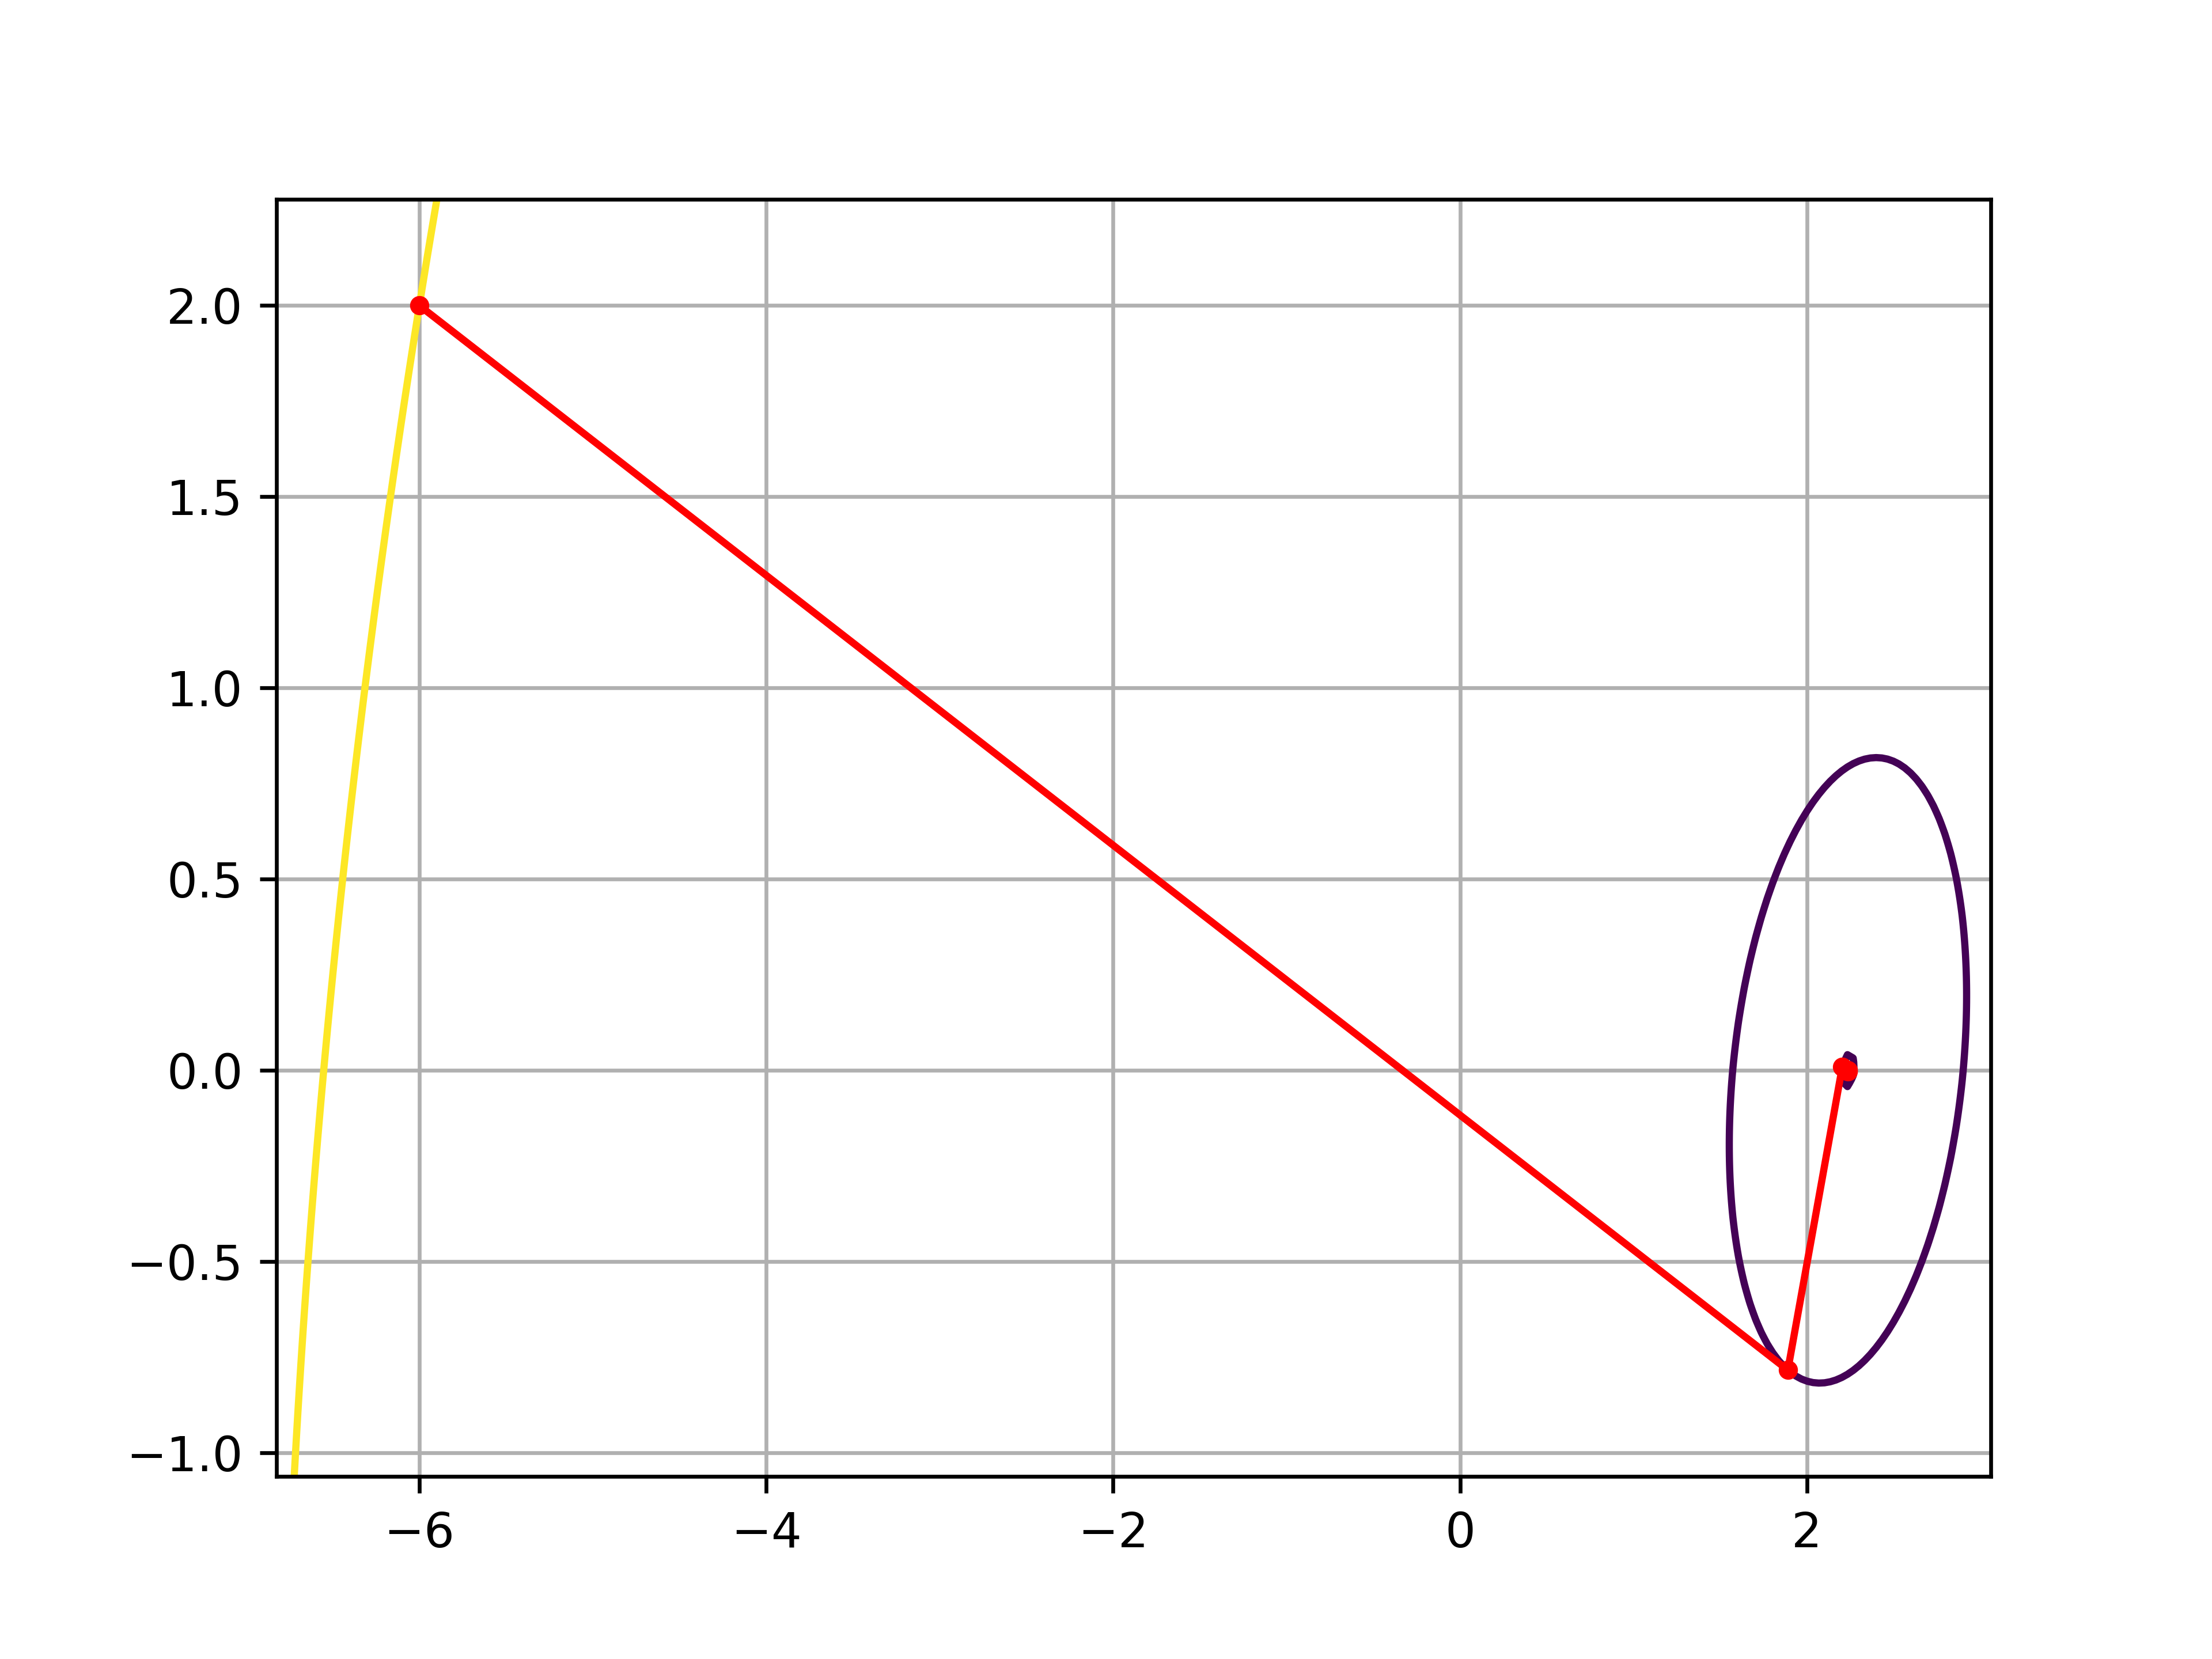
\includegraphics[width=0.85\textwidth]{Метод наискорейшего спуска, eps 0.01, start = (-6.00, 2.00), Квадратичная функция}%
	        \caption{Поиск минимума квадратичной функции при $\varepsilon = 0.01$, начальной точке (-6.0, 2.0) методом наискорейшего спуска}
	        \vspace*{-1.2cm}
            \end{figure}
            
            \begin{figure}[H]
	        \centering
	        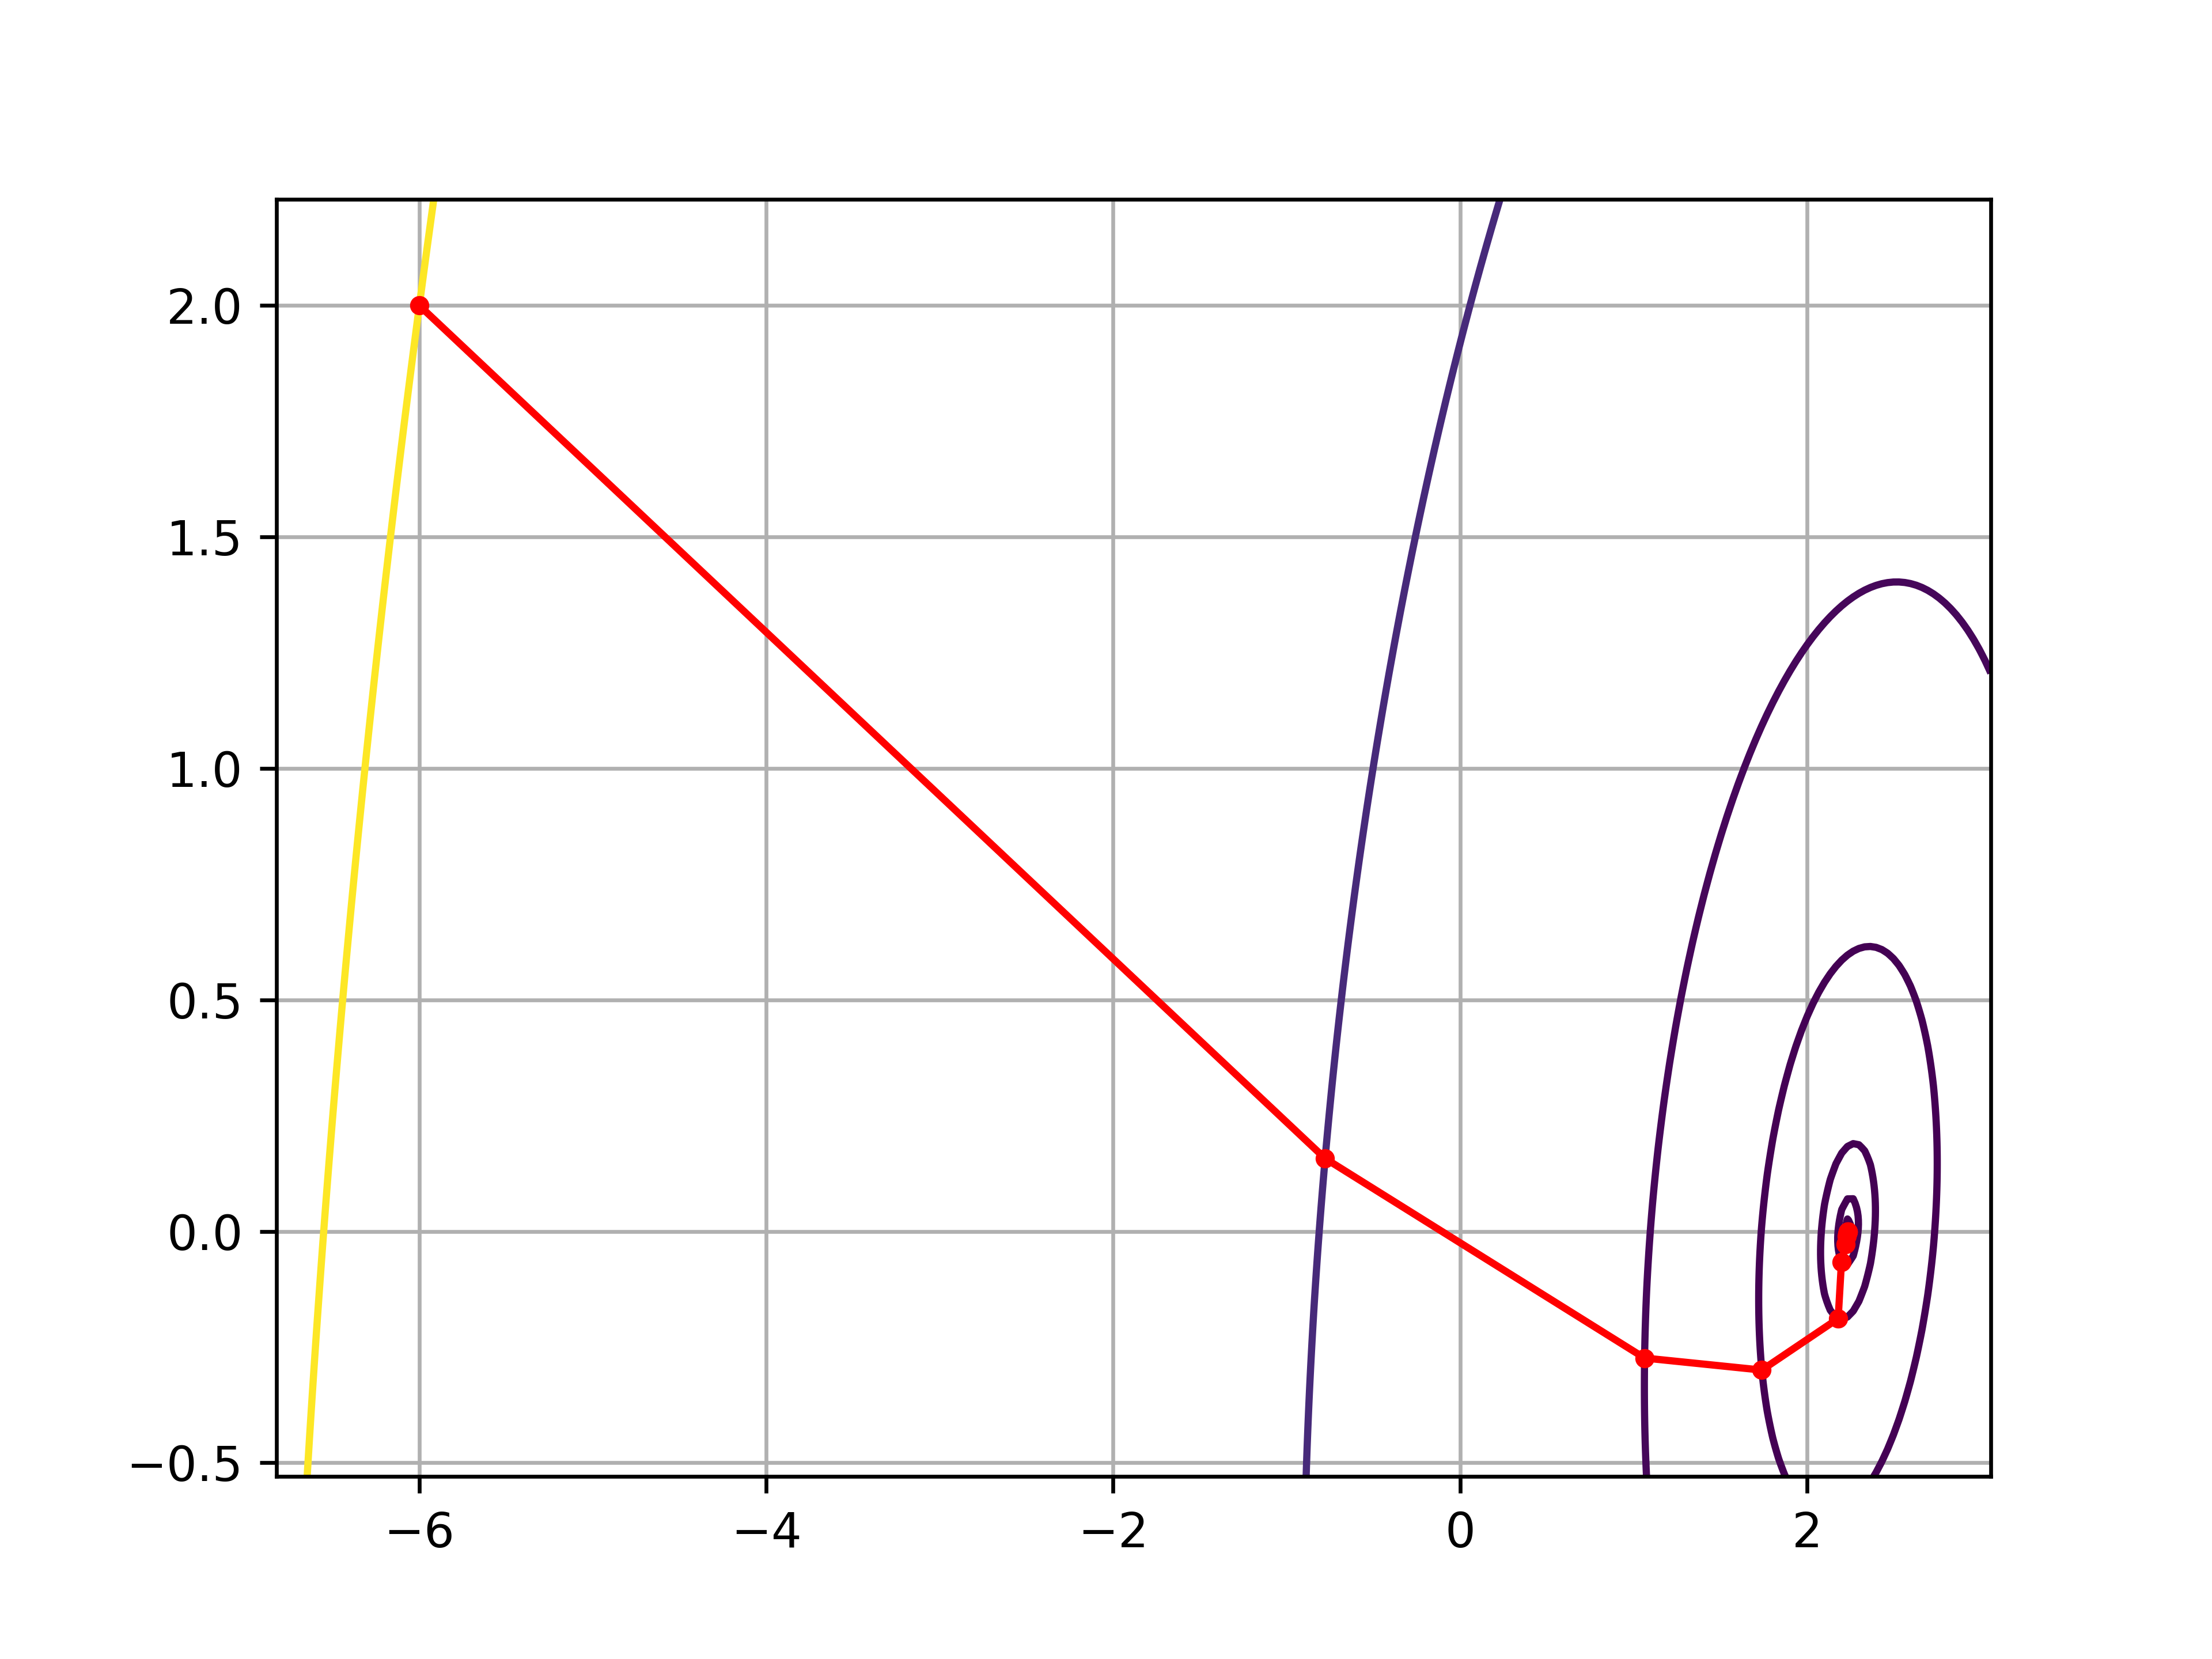
\includegraphics[width=0.85\textwidth]{Метод градиентного спуска с дробным шагом, eps 0.01, start = (-6.00, 2.00), Квадратичная функция}%
	        \caption{Поиск минимума квадратичной функции при $\varepsilon = 0.01$, начальной точке (-6.0, 2.0) методом градиентного спуска с дроблением шага}
	        \vspace*{-1.2cm}
            \end{figure}
            
            \begin{figure}[H]
	        \centering
	        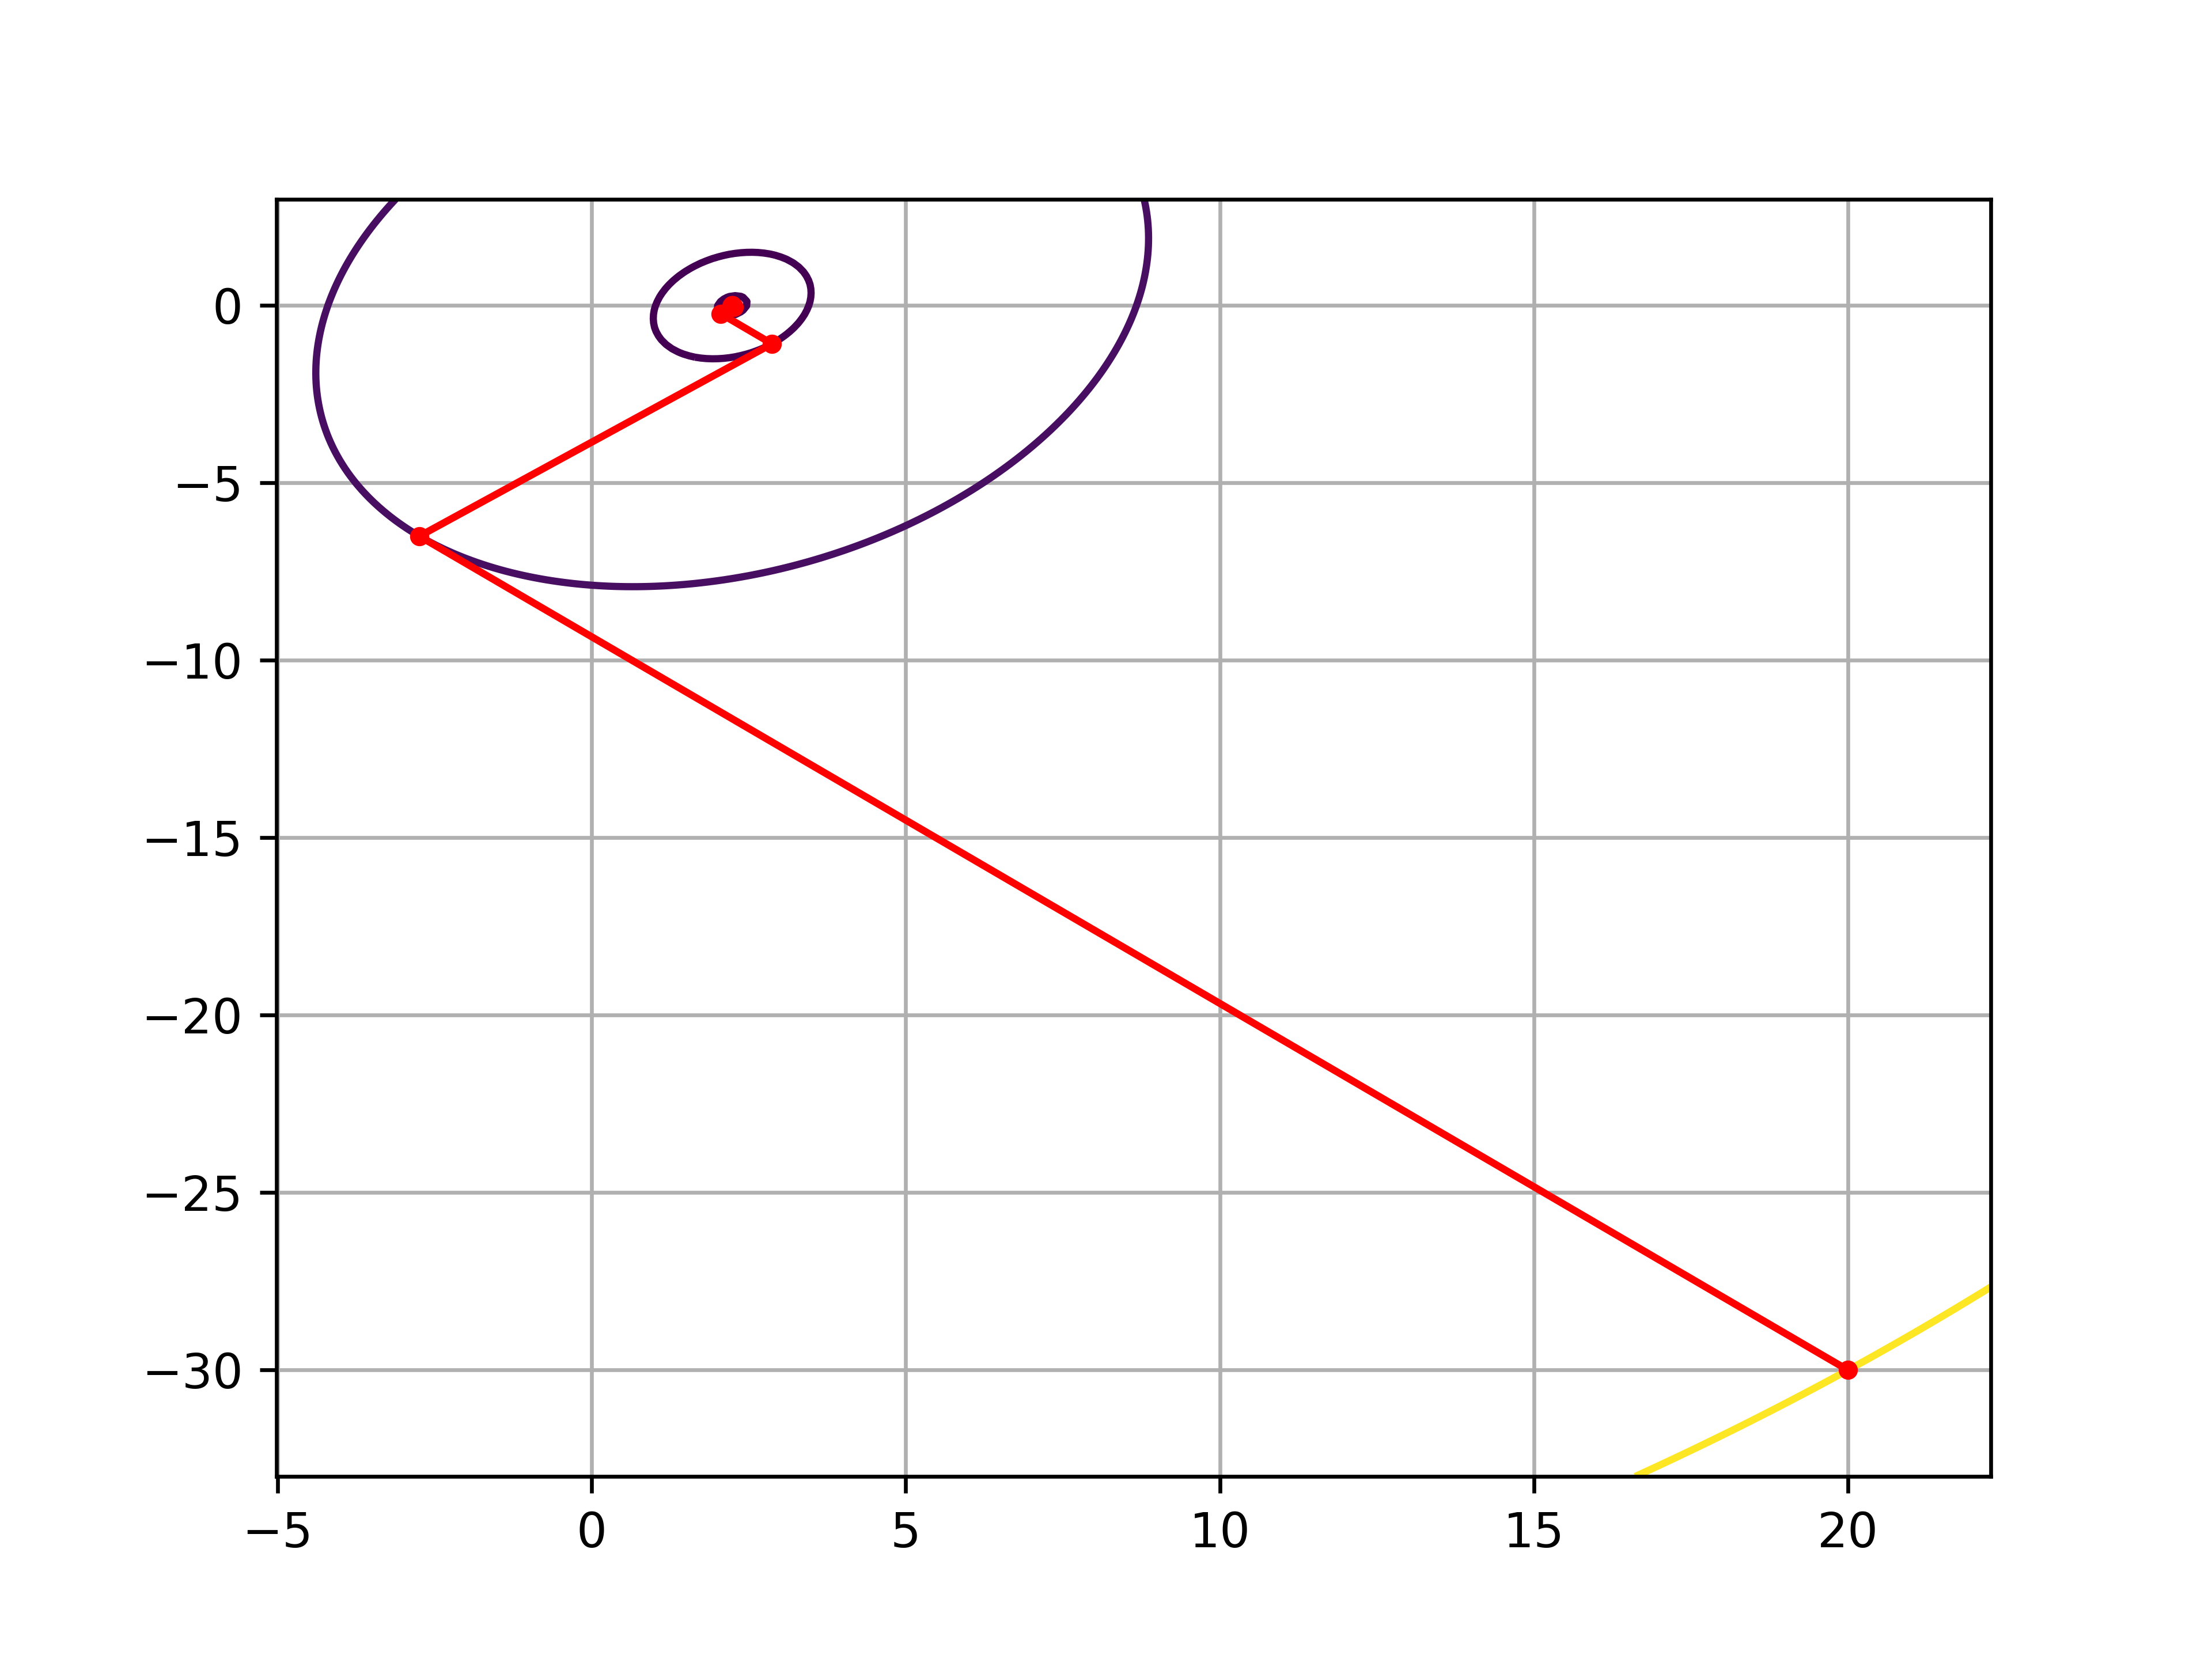
\includegraphics[width=0.85\textwidth]{Метод наискорейшего спуска, eps 0.01, start = (20.00, -30.00), Квадратичная функция}%
	        \caption{Поиск минимума квадратичной функции при $\varepsilon = 0.01$, начальной точке (20.0, -30.0) методом наискорейшего спуска}
	        \vspace*{-1.2cm}
            \end{figure}
            
            \begin{figure}[H]
	        \centering
	        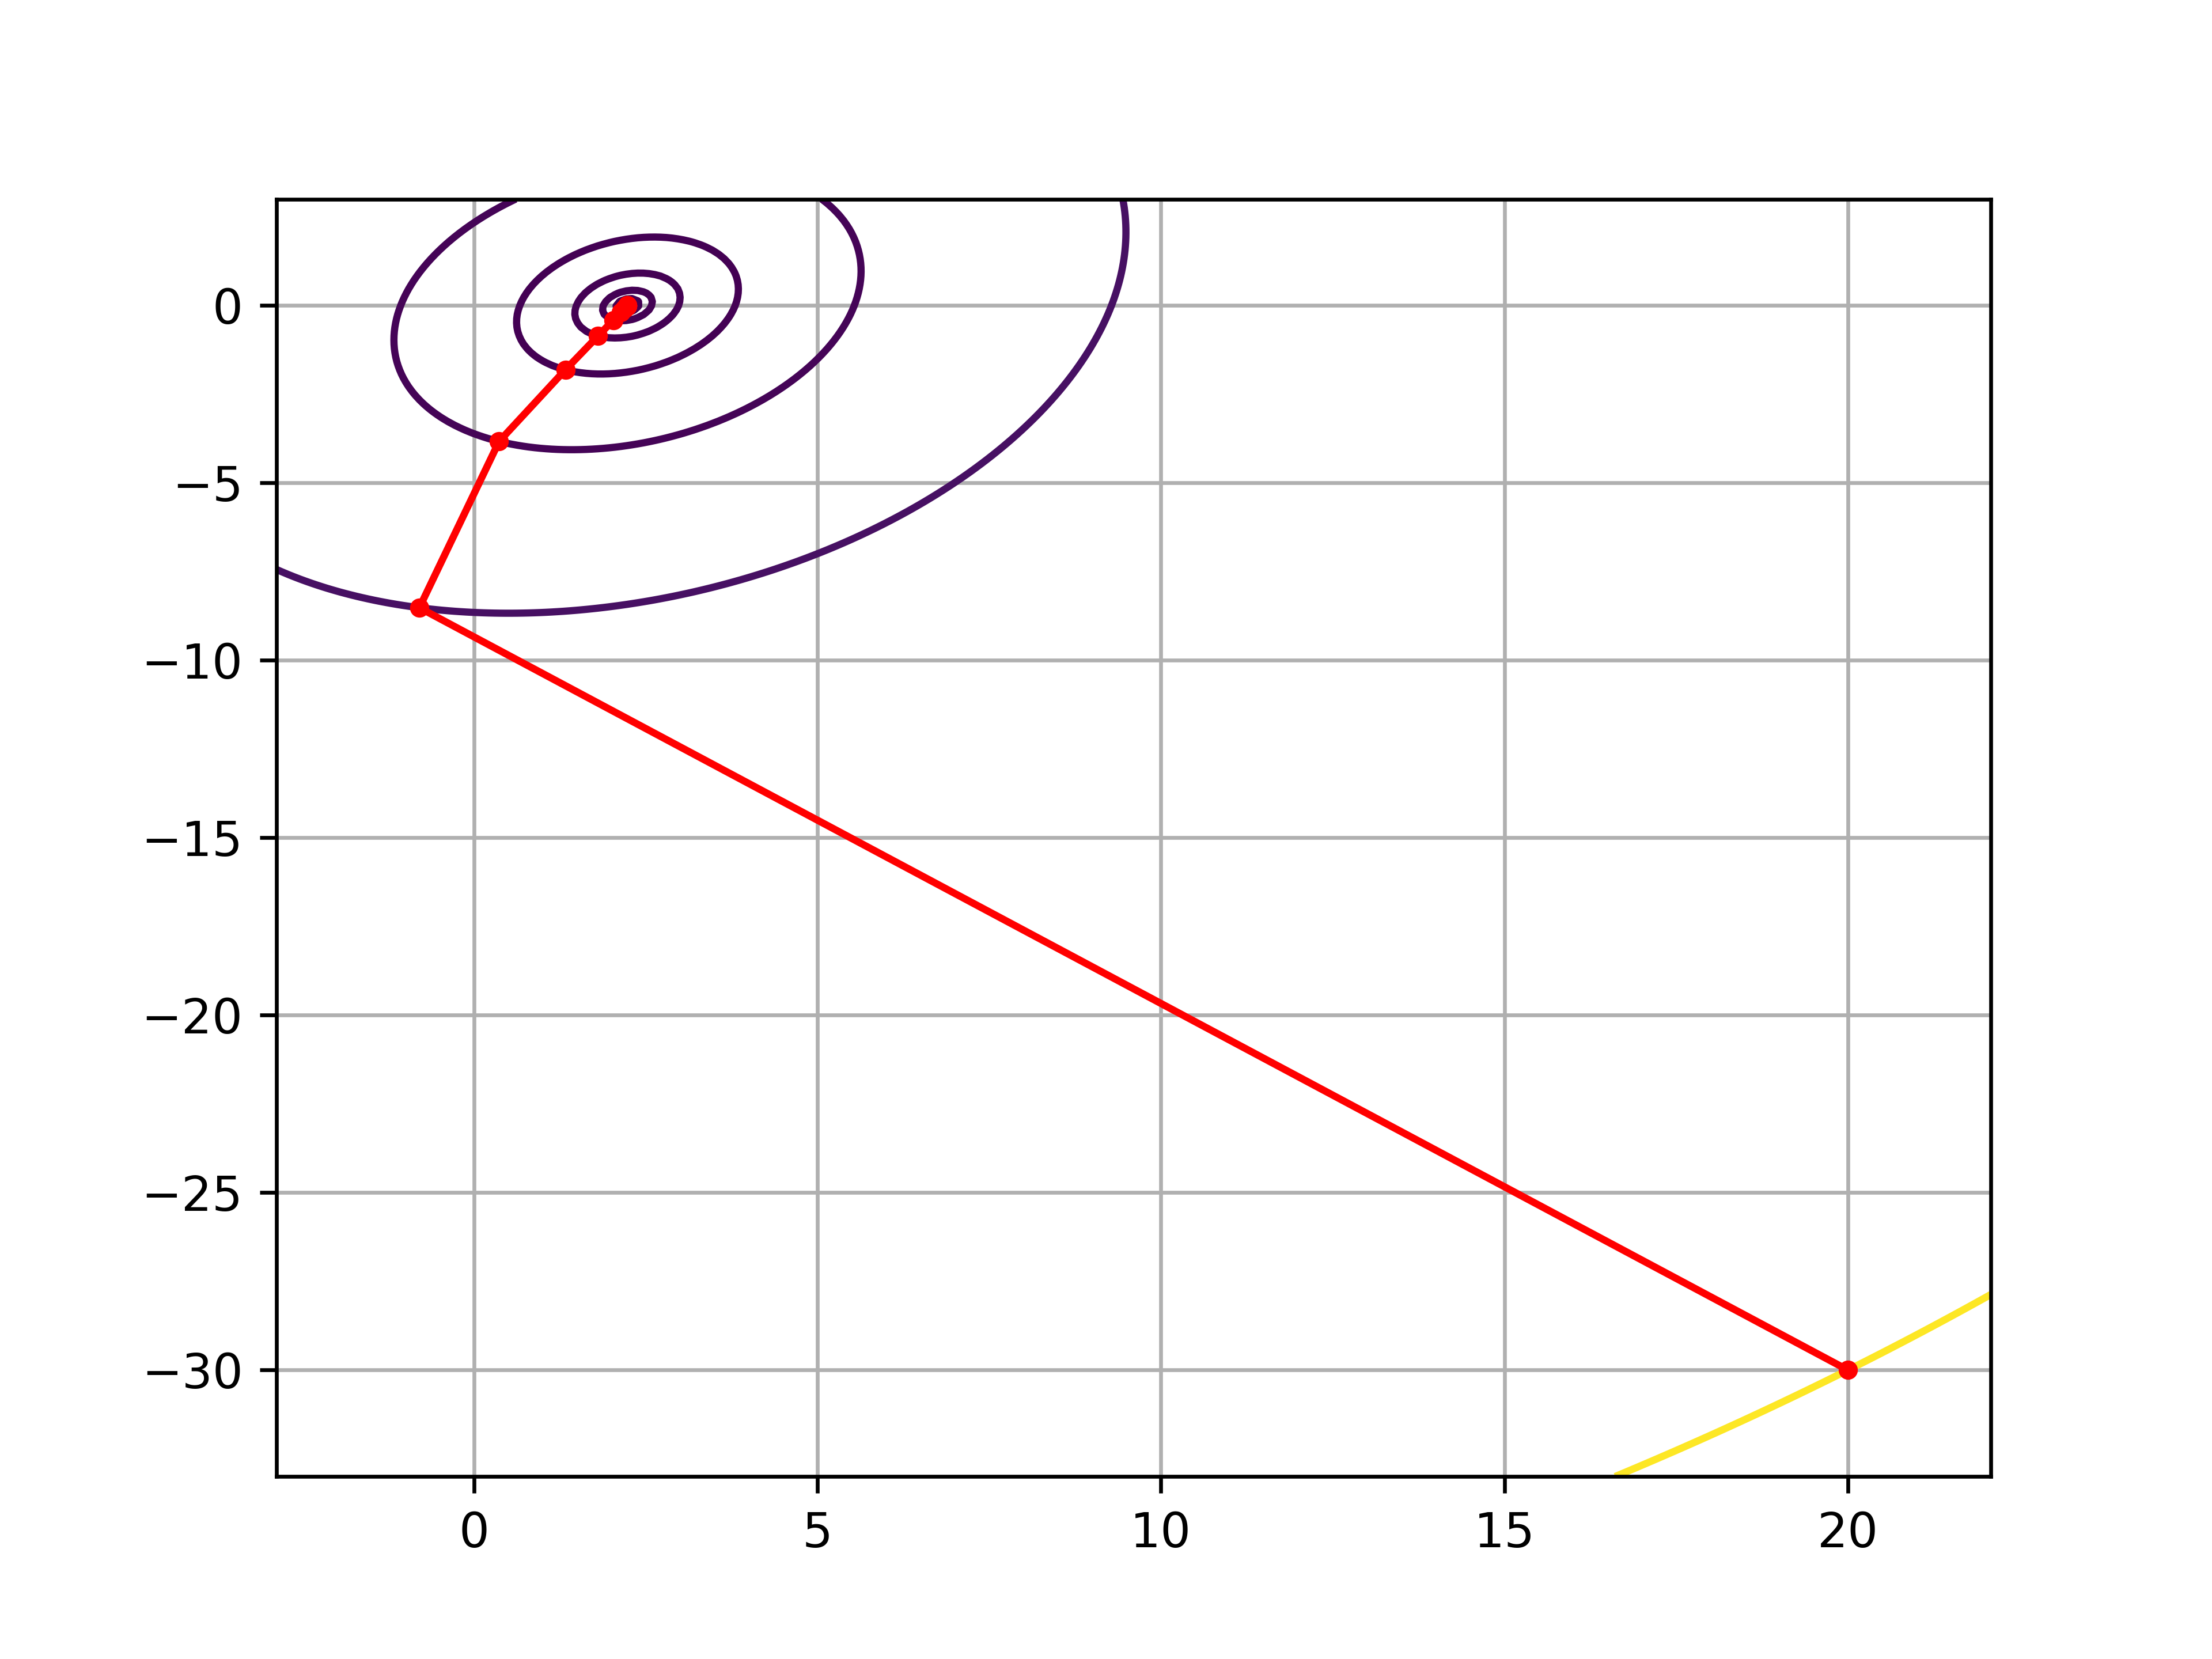
\includegraphics[width=0.85\textwidth]{Метод градиентного спуска с дробным шагом, eps 0.01, start = (20.00, -30.00), Квадратичная функция}%
	        \caption{Поиск минимума квадратичной функции при $\varepsilon = 0.01$, начальной точке (20.0, -30.0) методом градиентного спуска с дроблением шага}
	        \vspace*{-1.2cm}
            \end{figure}
            
            \begin{figure}[H]
	        \centering
	        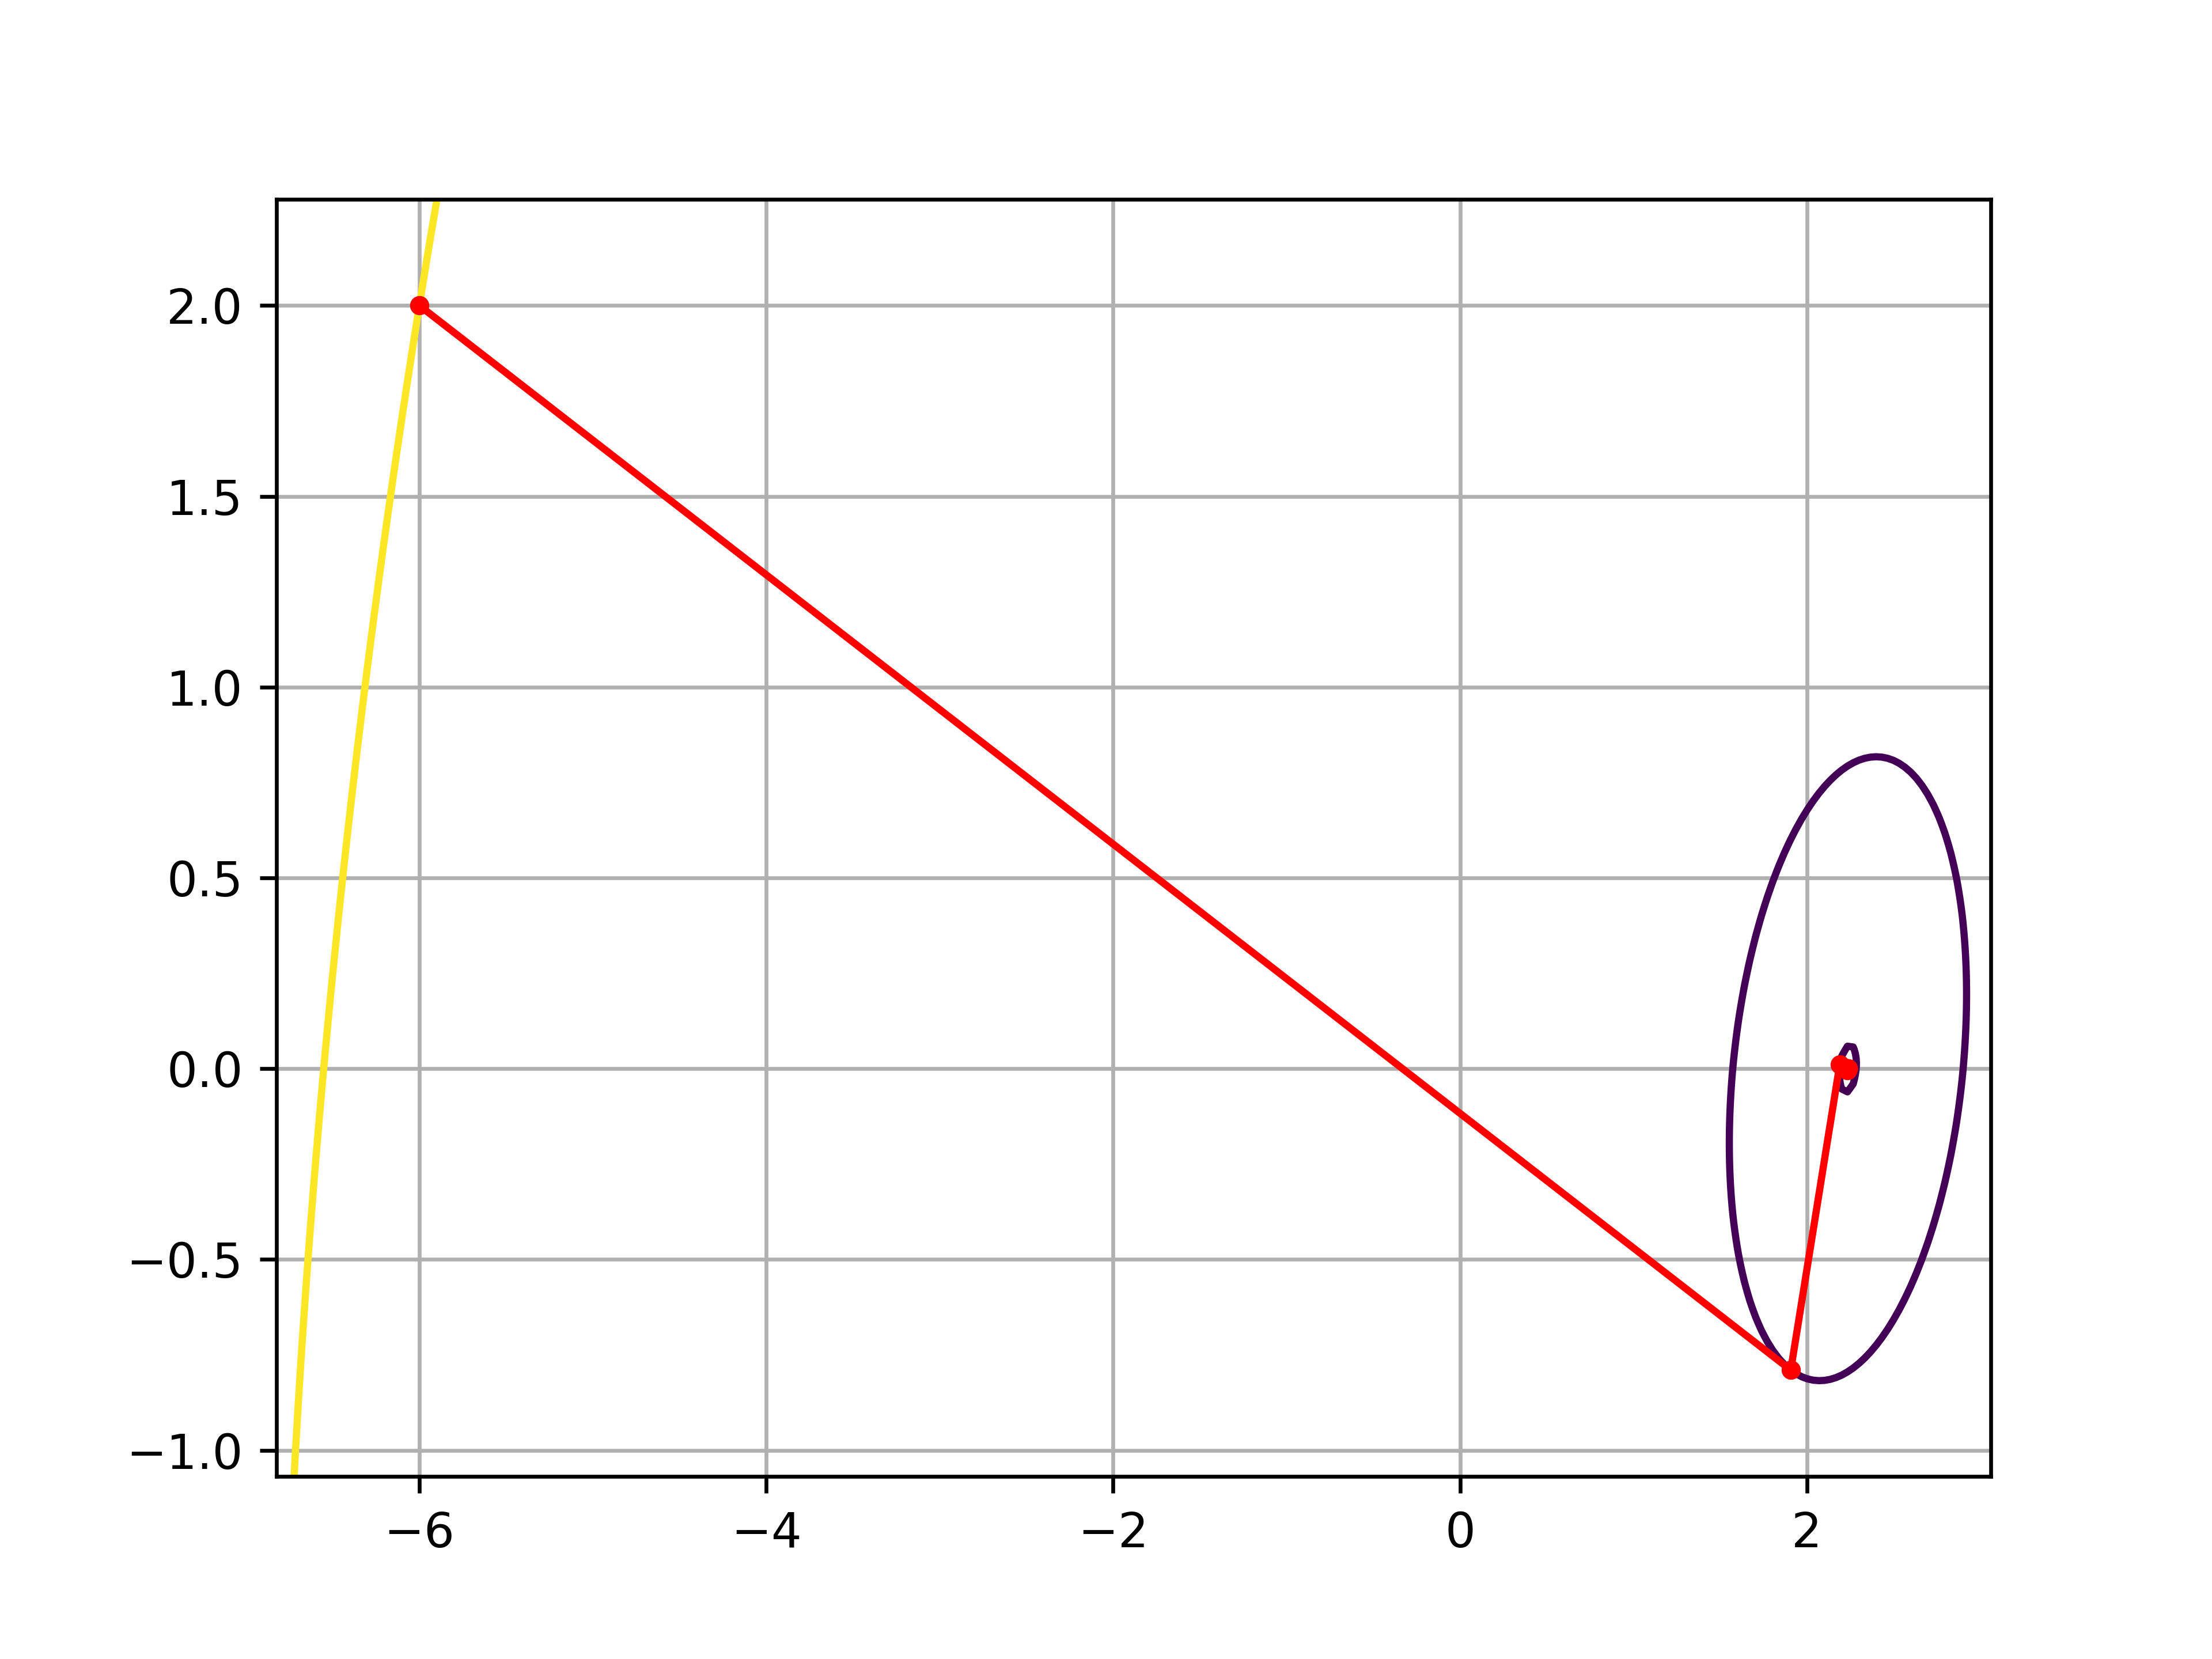
\includegraphics[width=0.85\textwidth]{Метод наискорейшего спуска, eps 1e-06, start = (-6.000000, 2.000000), Квадратичная функция}%
	        \caption{Поиск минимума квадратичной функции при $\varepsilon = 1e-06$, начальной точке (-6.0, 2.0) методом наискорейшего спуска}
	        \vspace*{-1.2cm}
            \end{figure}
            
            \begin{figure}[H]
	        \centering
	        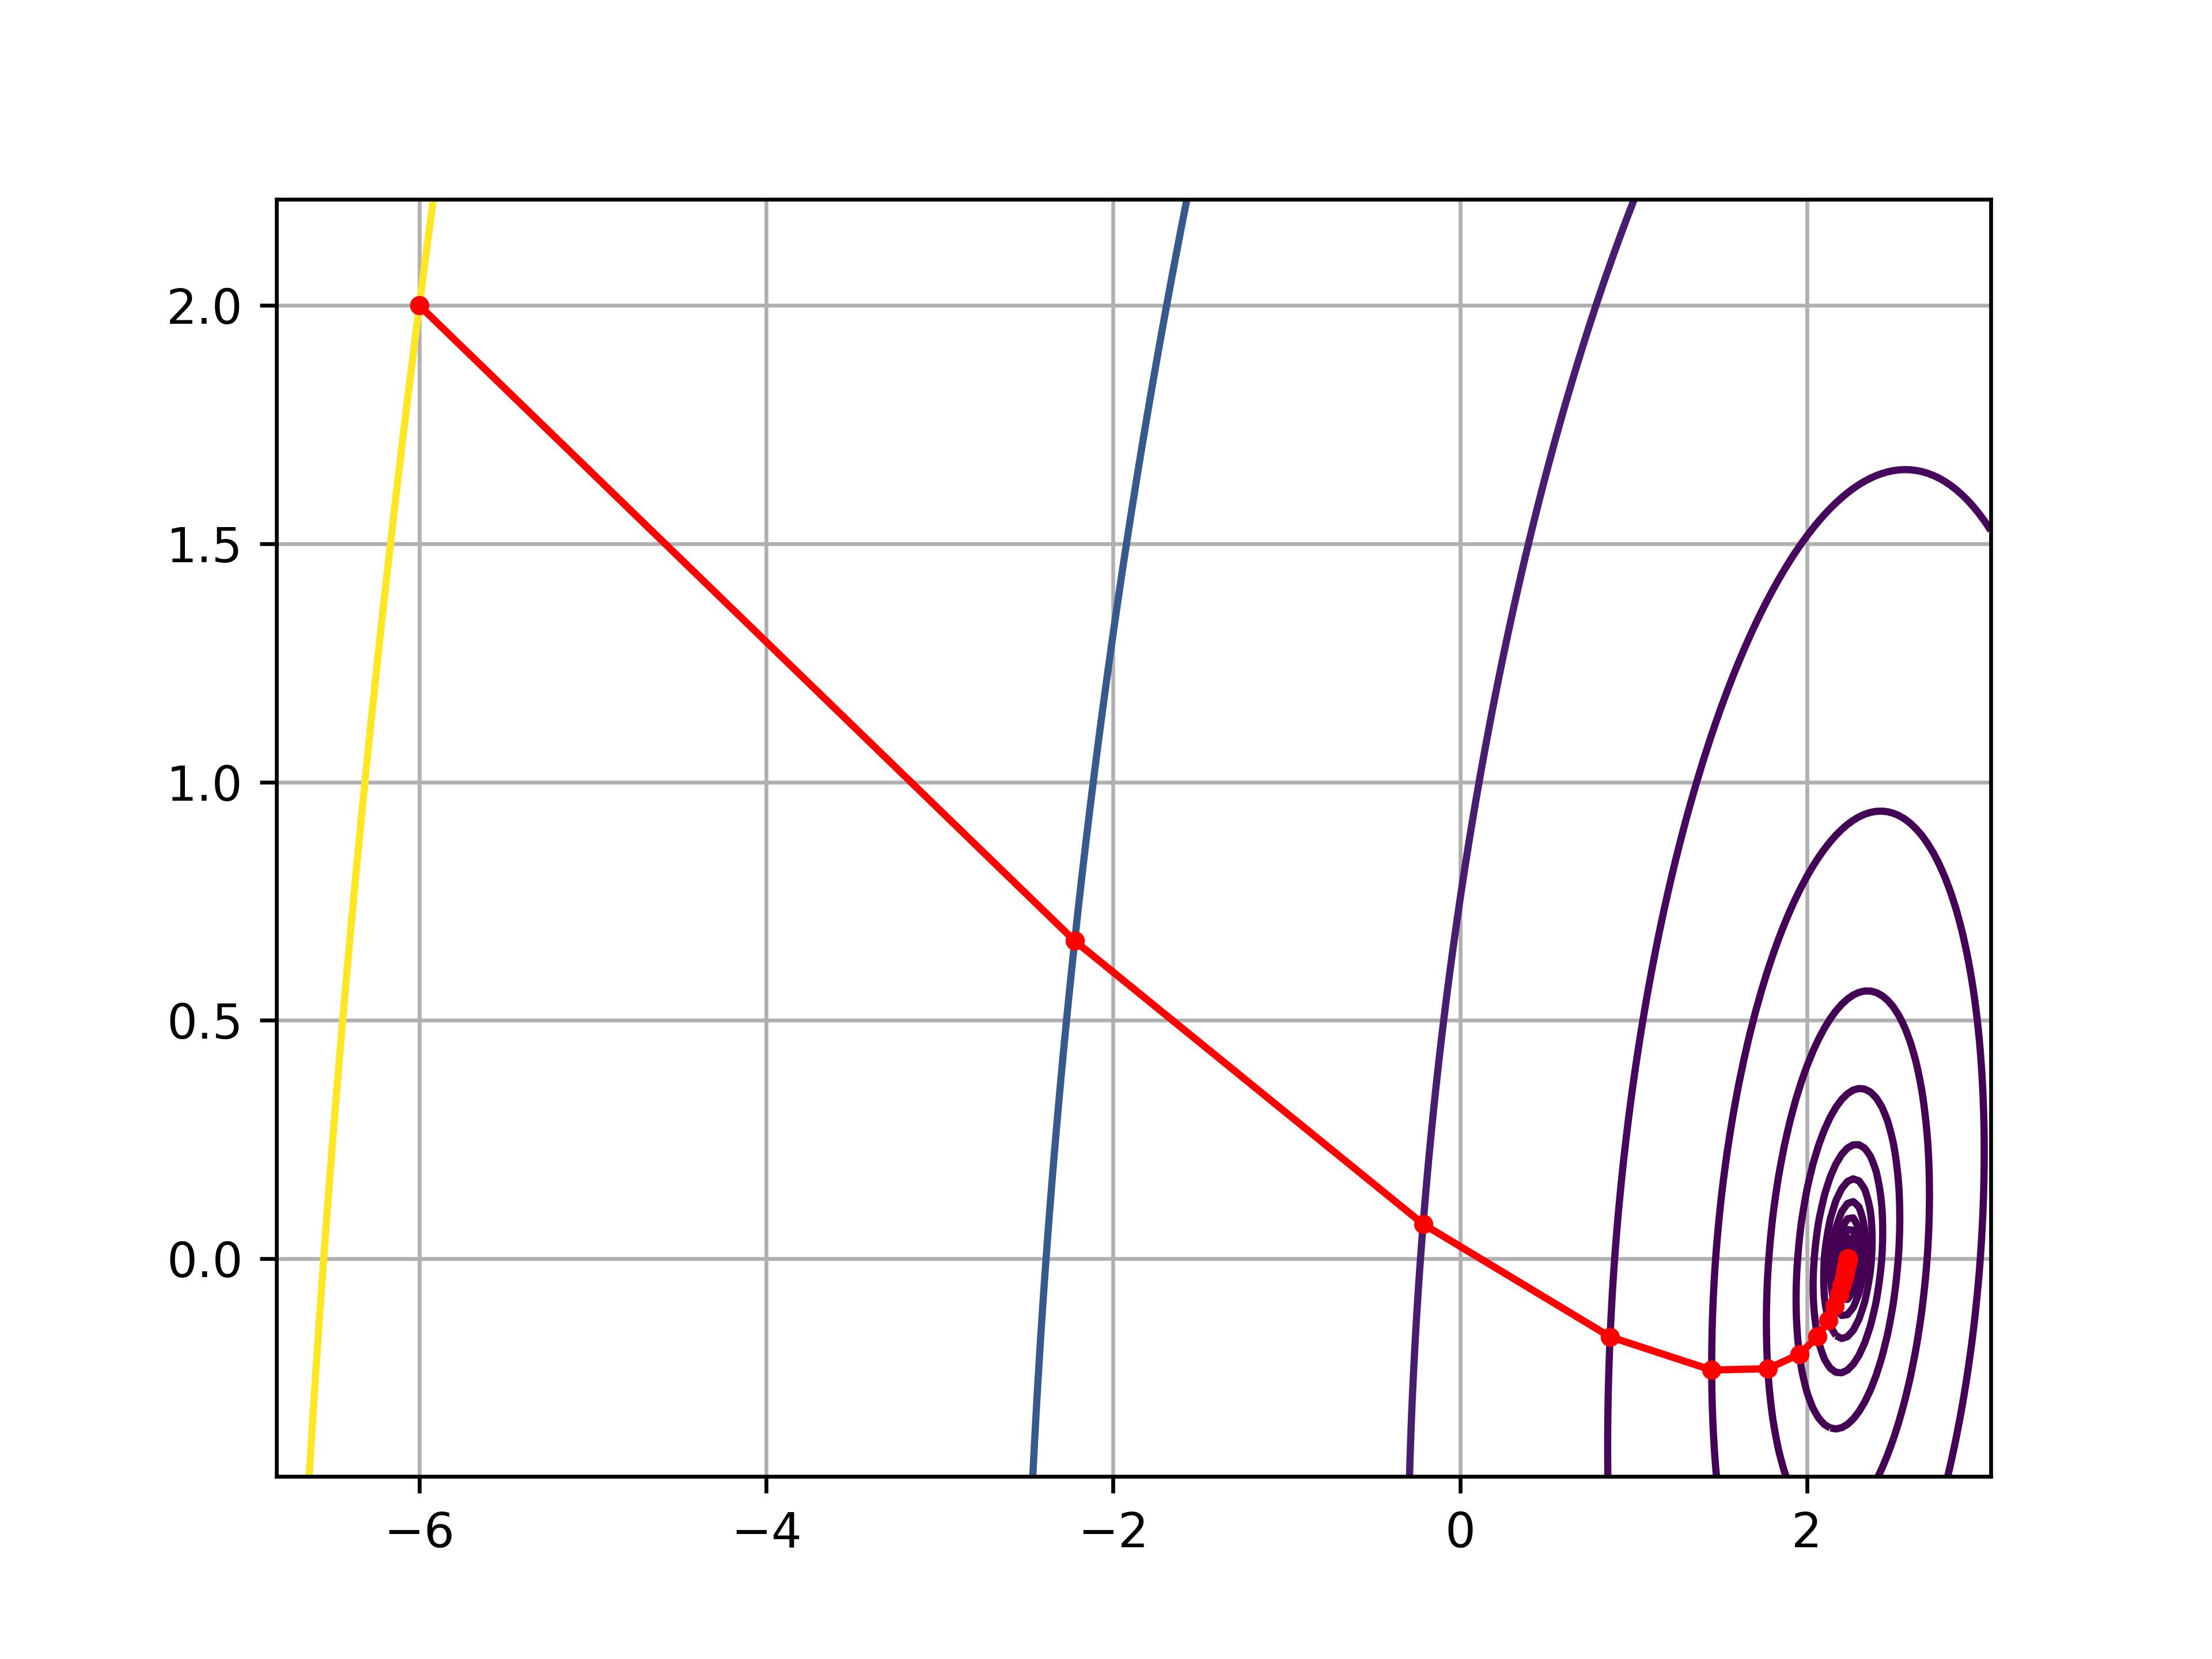
\includegraphics[width=0.85\textwidth]{Метод градиентного спуска с дробным шагом, eps 1e-06, start = (-6.000000, 2.000000), Квадратичная функция}%
	        \caption{Поиск минимума квадратичной функции при $\varepsilon = 1e-06$, начальной точке (-6.0, 2.0) методом градиентного спуска с дроблением шага}
	        \vspace*{-1.2cm}
            \end{figure}
            
            \begin{figure}[H]
	        \centering
	        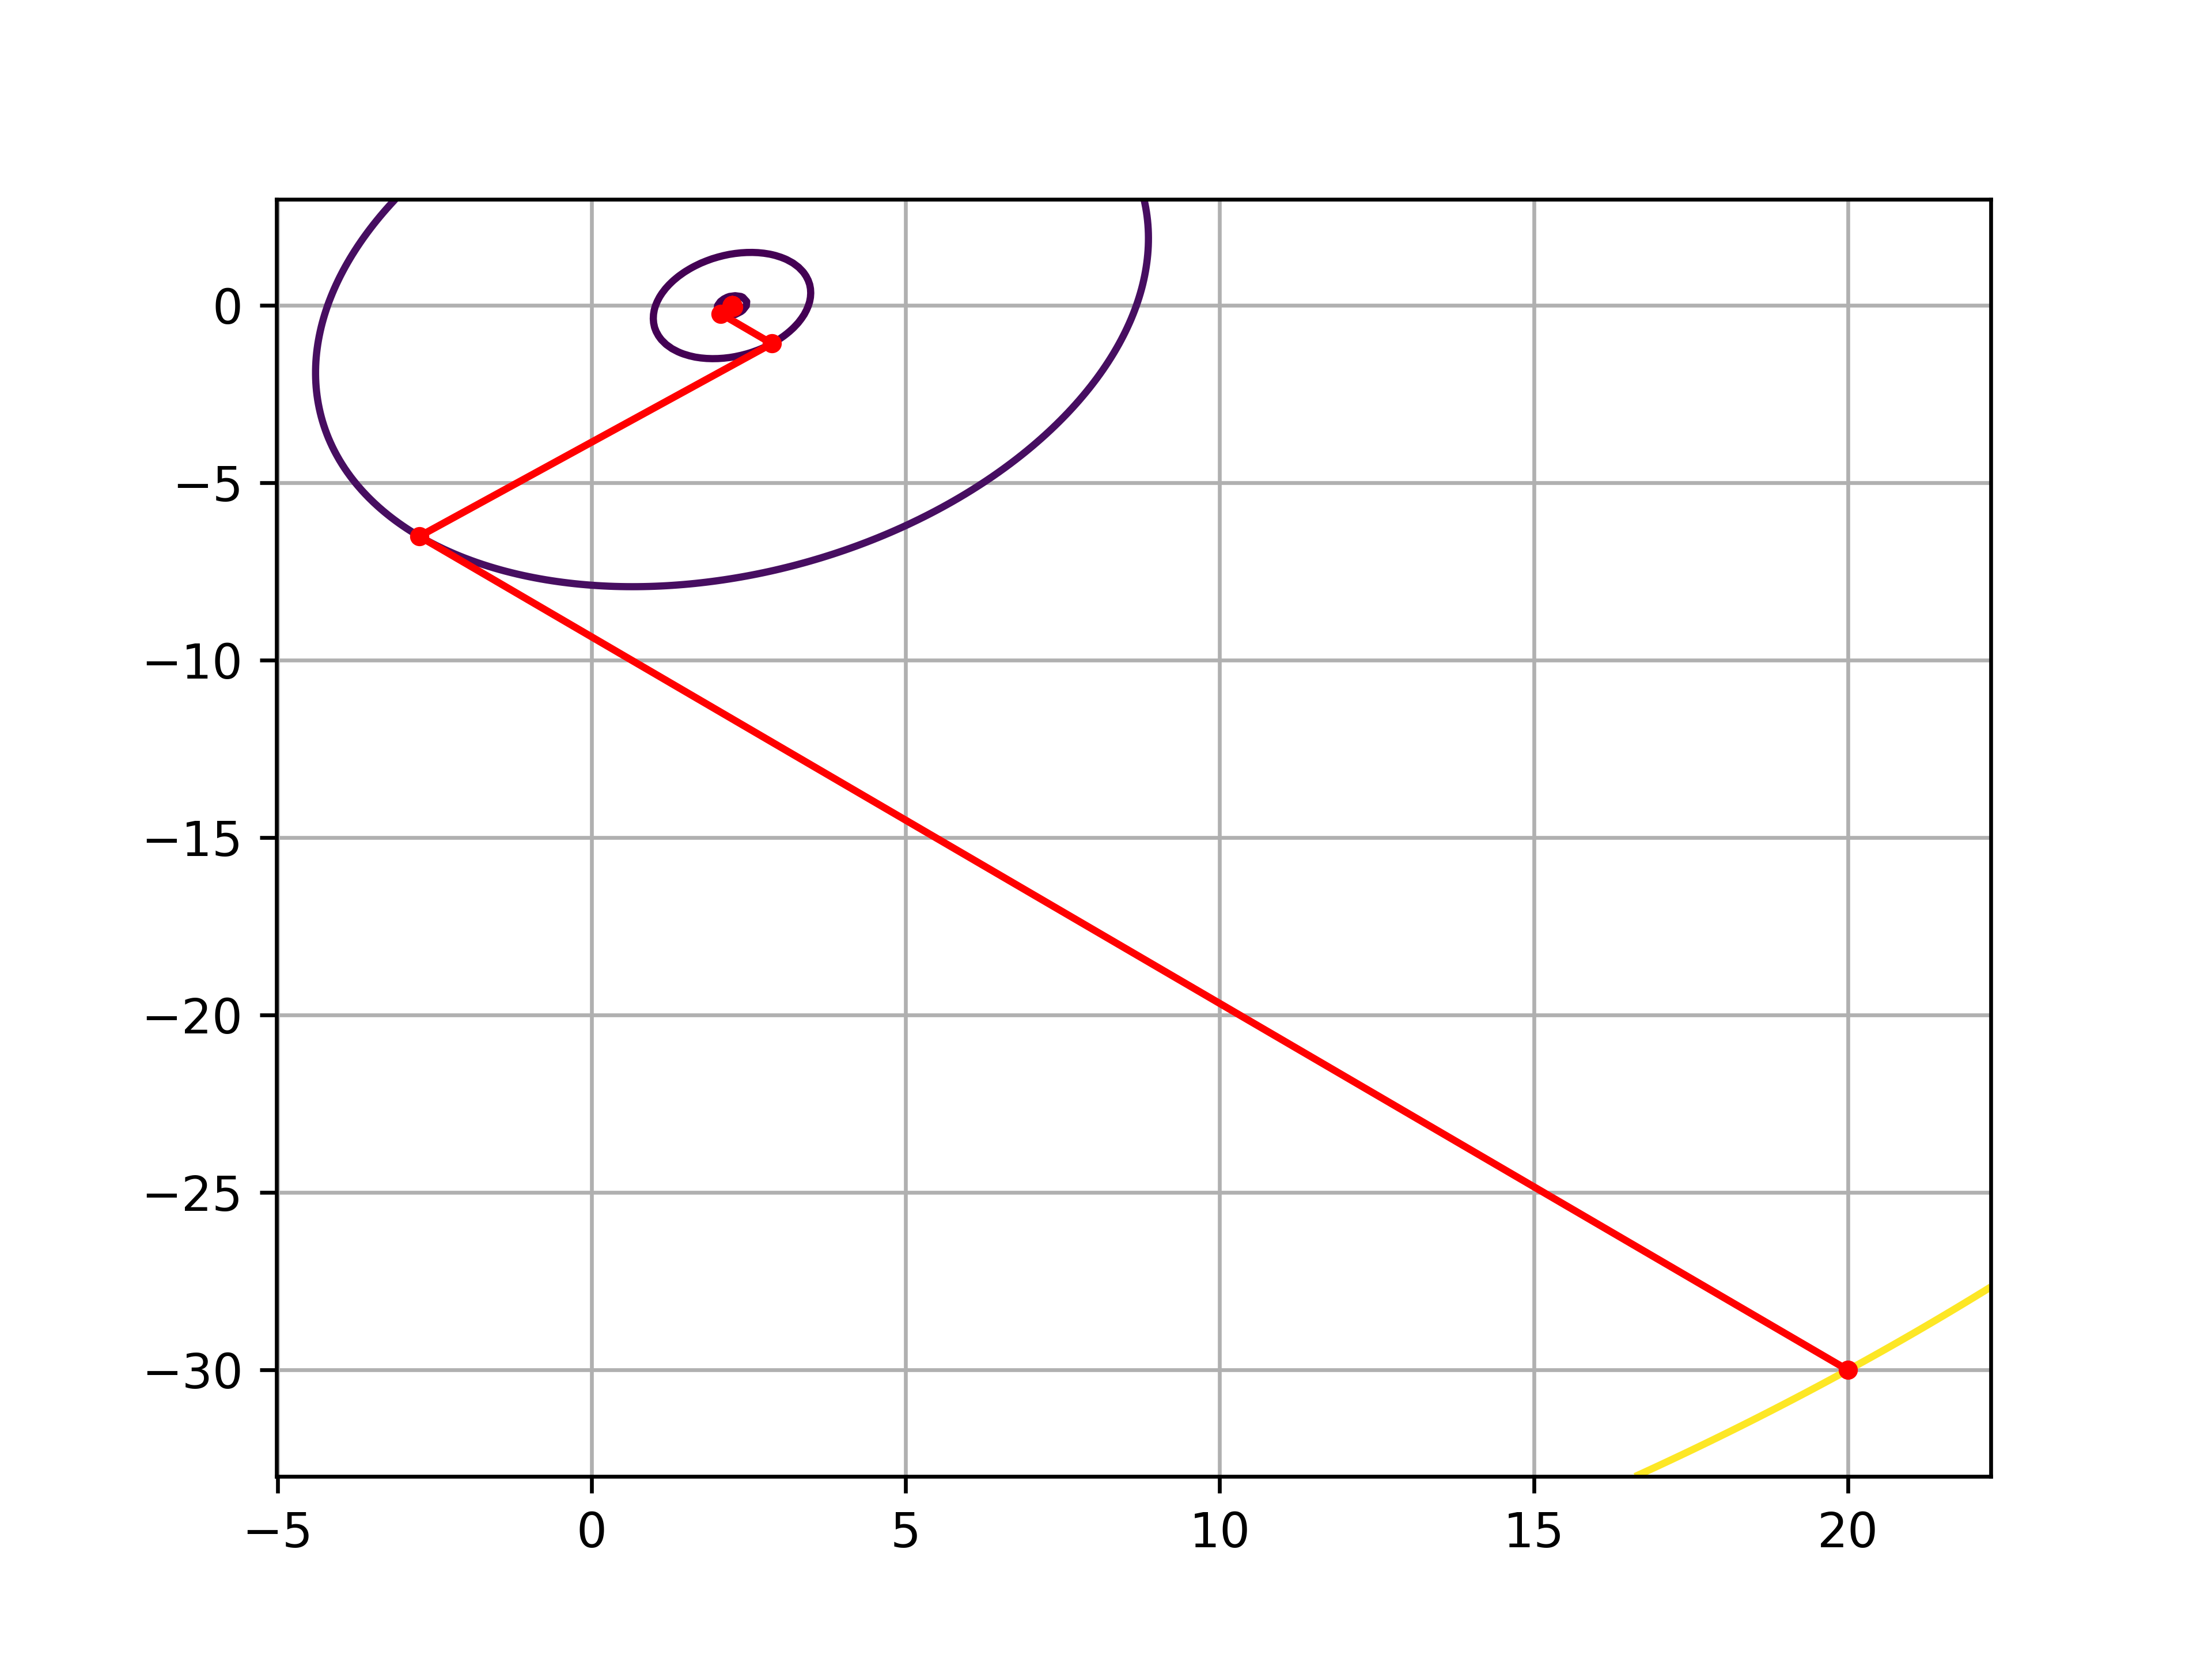
\includegraphics[width=0.85\textwidth]{Метод наискорейшего спуска, eps 1e-06, start = (20.000000, -30.000000), Квадратичная функция}%
	        \caption{Поиск минимума квадратичной функции при $\varepsilon = 1e-06$, начальной точке (20.0, -30.0) методом наискорейшего спуска}
	        \vspace*{-1.2cm}
            \end{figure}
            
            \begin{figure}[H]
	        \centering
	        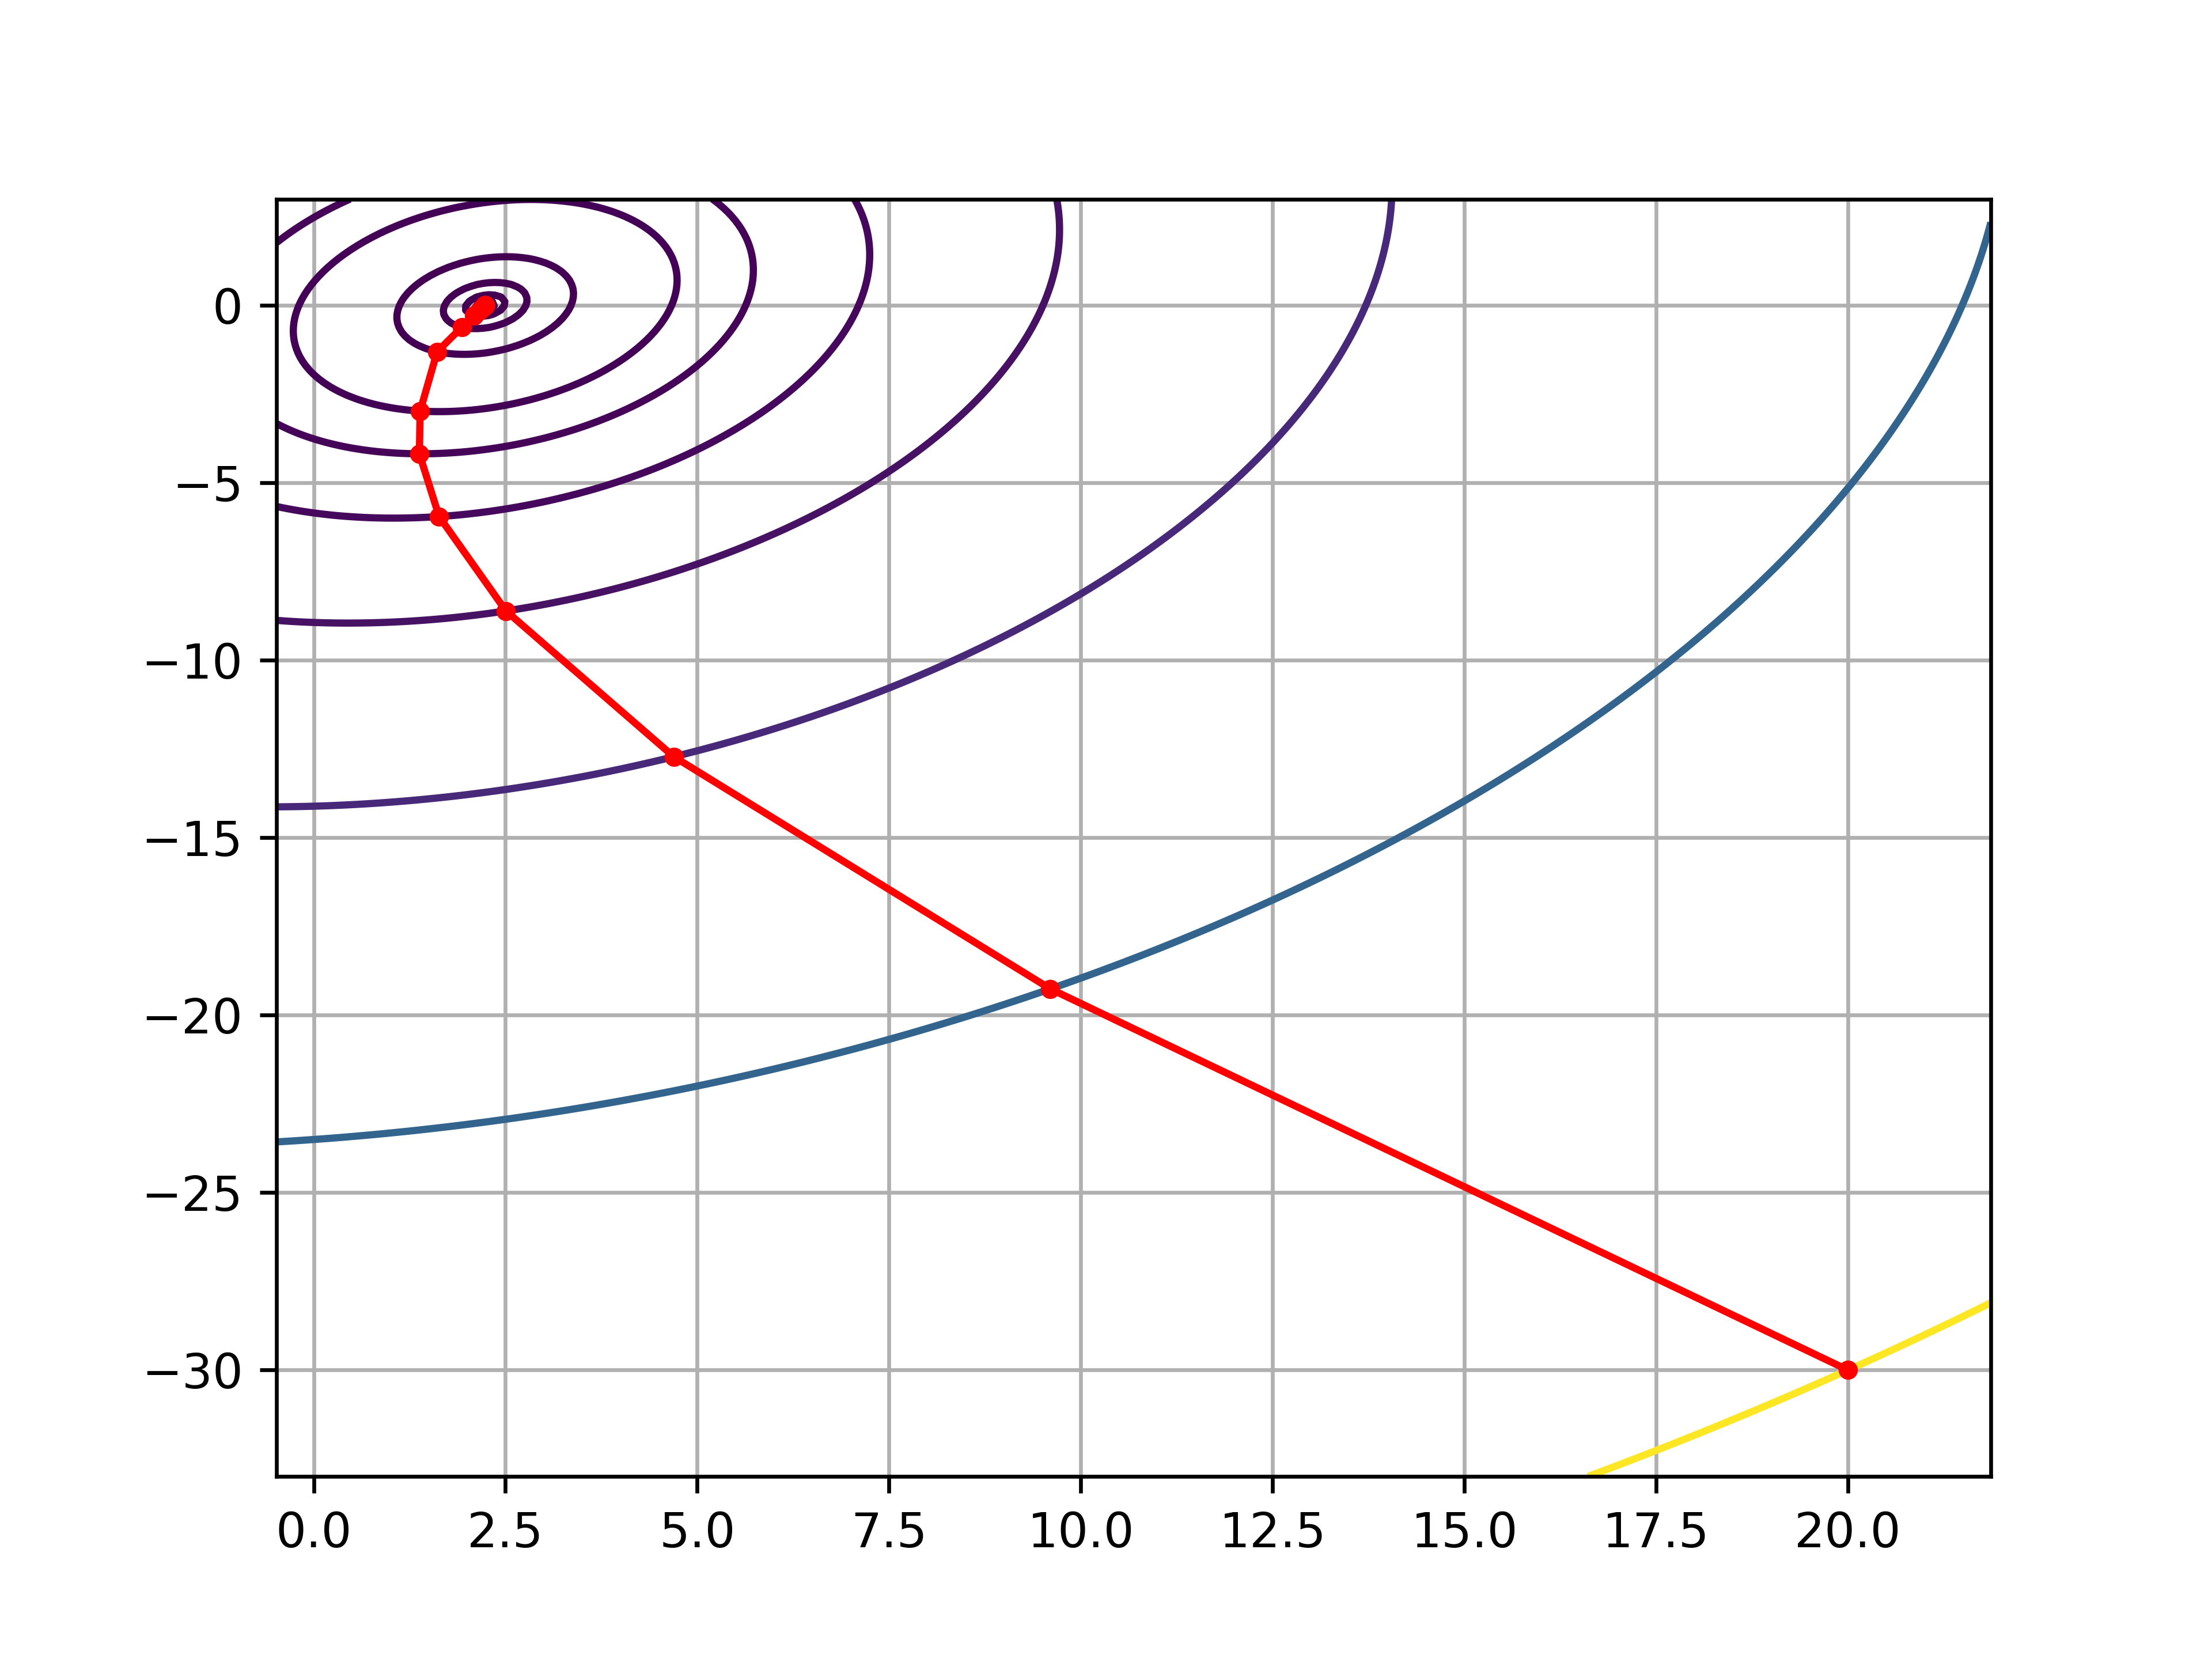
\includegraphics[width=0.85\textwidth]{Метод градиентного спуска с дробным шагом, eps 1e-06, start = (20.000000, -30.000000), Квадратичная функция}%
	        \caption{Поиск минимума квадратичной функции при $\varepsilon = 1e-06$, начальной точке (20.0, -30.0) методом градиентного спуска с дроблением шага}
	        \vspace*{-1.2cm}
            \end{figure}
            \subsubsection{Функция Розенброка с $\alpha$ = 1}

\begin{table}[H]
        \centering
        \vspace*{-1.5em}
        \caption{Результаты работы алгоритмов\\для функции Розенброка с $\alpha$ = 1}
        \footnotesize
        \begin{tabular}{|c|c|c|c|}
        \hline
        & &\makecell{Метод наискорейшего\\спуска} &\makecell{Метод градиентного спуска\\с дроблением шага} \\
        \hline
	\multirow{10}{*}{\rotatebox[origin=c]{90}{$\varepsilon = 0.01$}}&\textbf{Начальная точка} &\multicolumn{2}{c|}{\textbf{(-6.00, 2.00)}}\\
	\cline{2-4}
	&Точка минимума &(1.01, 1.02) &(1.01, 1.02) \\ 
	\cline{2-4}
	&Минимум &0.00 &0.00 \\ 
	\cline{2-4}
	&Кол-во итераций &107 &33 \\ 
	\cline{2-4}
	&\makecell{Кол-во вызовов\\целевой функции} &1960 &268 \\ 
	\cline{2-4}
	&\makecell{Кол-во вычислений\\градиента} &107 &33 \\ 
	\cline{2-4}
\cline{2-4}&\textbf{Начальная точка} &\multicolumn{2}{c|}{\textbf{(20.00, -30.00)}}\\
	\cline{2-4}
	&Точка минимума &(1.01, 1.02) &(1.00, 0.99) \\ 
	\cline{2-4}
	&Минимум &0.00 &0.00 \\ 
	\cline{2-4}
	&Кол-во итераций &98 &35 \\ 
	\cline{2-4}
	&\makecell{Кол-во вызовов\\целевой функции} &1765 &320 \\ 
	\cline{2-4}
	&\makecell{Кол-во вычислений\\градиента} &98 &35 \\ 
	\cline{2-4}
	\hline
	\multirow{10}{*}{\rotatebox[origin=c]{90}{$\varepsilon = 1e-06$}}&\textbf{Начальная точка} &\multicolumn{2}{c|}{\textbf{(-6.000000, 2.000000)}}\\
	\cline{2-4}
	&Точка минимума &(1.000001, 1.000002) &(1.000000, 1.000001) \\ 
	\cline{2-4}
	&Минимум &0.000000 &0.000000 \\ 
	\cline{2-4}
	&Кол-во итераций &172 &69 \\ 
	\cline{2-4}
	&\makecell{Кол-во вызовов\\целевой функции} &6304 &512 \\ 
	\cline{2-4}
	&\makecell{Кол-во вычислений\\градиента} &172 &69 \\ 
	\cline{2-4}
\cline{2-4}&\textbf{Начальная точка} &\multicolumn{2}{c|}{\textbf{(20.000000, -30.000000)}}\\
	\cline{2-4}
	&Точка минимума &(0.999999, 0.999998) &(1.000000, 0.999999) \\ 
	\cline{2-4}
	&Минимум &0.000000 &0.000000 \\ 
	\cline{2-4}
	&Кол-во итераций &102 &55 \\ 
	\cline{2-4}
	&\makecell{Кол-во вызовов\\целевой функции} &3718 &441 \\ 
	\cline{2-4}
	&\makecell{Кол-во вычислений\\градиента} &102 &55 \\ 
	\cline{2-4}
	\hline

\end{tabular}
\end{table}


            \begin{figure}[H]
	        \centering
	        \includegraphics[width=0.85\textwidth]{Метод наискорейшего спуска, eps 0.01, start = (-6.00, 2.00), Функция Розенброка с alpha = 1}%
	        \caption{Поиск минимума функции Розенброка с $\alpha$ = 1 при $\varepsilon = 0.01$, начальной точке (-6.0, 2.0) методом наискорейшего спуска}
	        \vspace*{-1.2cm}
            \end{figure}
            
            \begin{figure}[H]
	        \centering
	        \includegraphics[width=0.85\textwidth]{Метод градиентного спуска с дробным шагом, eps 0.01, start = (-6.00, 2.00), Функция Розенброка с alpha = 1}%
	        \caption{Поиск минимума функции Розенброка с $\alpha$ = 1 при $\varepsilon = 0.01$, начальной точке (-6.0, 2.0) методом градиентного спуска с дроблением шага}
	        \vspace*{-1.2cm}
            \end{figure}
            
            \begin{figure}[H]
	        \centering
	        \includegraphics[width=0.85\textwidth]{Метод наискорейшего спуска, eps 0.01, start = (20.00, -30.00), Функция Розенброка с alpha = 1}%
	        \caption{Поиск минимума функции Розенброка с $\alpha$ = 1 при $\varepsilon = 0.01$, начальной точке (20.0, -30.0) методом наискорейшего спуска}
	        \vspace*{-1.2cm}
            \end{figure}
            
            \begin{figure}[H]
	        \centering
	        \includegraphics[width=0.85\textwidth]{Метод градиентного спуска с дробным шагом, eps 0.01, start = (20.00, -30.00), Функция Розенброка с alpha = 1}%
	        \caption{Поиск минимума функции Розенброка с $\alpha$ = 1 при $\varepsilon = 0.01$, начальной точке (20.0, -30.0) методом градиентного спуска с дроблением шага}
	        \vspace*{-1.2cm}
            \end{figure}
            
            \begin{figure}[H]
	        \centering
	        \includegraphics[width=0.85\textwidth]{Метод наискорейшего спуска, eps 1e-06, start = (-6.000000, 2.000000), Функция Розенброка с alpha = 1}%
	        \caption{Поиск минимума функции Розенброка с $\alpha$ = 1 при $\varepsilon = 1e-06$, начальной точке (-6.0, 2.0) методом наискорейшего спуска}
	        \vspace*{-1.2cm}
            \end{figure}
            
            \begin{figure}[H]
	        \centering
	        \includegraphics[width=0.85\textwidth]{Метод градиентного спуска с дробным шагом, eps 1e-06, start = (-6.000000, 2.000000), Функция Розенброка с alpha = 1}%
	        \caption{Поиск минимума функции Розенброка с $\alpha$ = 1 при $\varepsilon = 1e-06$, начальной точке (-6.0, 2.0) методом градиентного спуска с дроблением шага}
	        \vspace*{-1.2cm}
            \end{figure}
            
            \begin{figure}[H]
	        \centering
	        \includegraphics[width=0.85\textwidth]{Метод наискорейшего спуска, eps 1e-06, start = (20.000000, -30.000000), Функция Розенброка с alpha = 1}%
	        \caption{Поиск минимума функции Розенброка с $\alpha$ = 1 при $\varepsilon = 1e-06$, начальной точке (20.0, -30.0) методом наискорейшего спуска}
	        \vspace*{-1.2cm}
            \end{figure}
            
            \begin{figure}[H]
	        \centering
	        \includegraphics[width=0.85\textwidth]{Метод градиентного спуска с дробным шагом, eps 1e-06, start = (20.000000, -30.000000), Функция Розенброка с alpha = 1}%
	        \caption{Поиск минимума функции Розенброка с $\alpha$ = 1 при $\varepsilon = 1e-06$, начальной точке (20.0, -30.0) методом градиентного спуска с дроблением шага}
	        \vspace*{-1.2cm}
            \end{figure}
            \subsubsection{Функция Розенброка с $\alpha$ = 10}

\begin{table}[H]
        \centering
        \vspace*{-1.5em}
        \caption{Результаты работы алгоритмов\\для функции Розенброка с $\alpha$ = 10}
        \footnotesize
        \begin{tabular}{|c|c|c|c|}
        \hline
        & &\makecell{Метод наискорейшего\\спуска} &\makecell{Метод градиентного спуска\\с дроблением шага} \\
        \hline
	\multirow{10}{*}{\rotatebox[origin=c]{90}{$\varepsilon = 0.01$}}&\textbf{Начальная точка} &\multicolumn{2}{c|}{\textbf{(-6.00, 2.00)}}\\
	\cline{2-4}
	&Точка минимума &(1.01, 1.02) &(1.01, 1.02) \\ 
	\cline{2-4}
	&Минимум &0.00 &0.00 \\ 
	\cline{2-4}
	&Кол-во итераций &191 &263 \\ 
	\cline{2-4}
	&\makecell{Кол-во вызовов\\целевой функции} &4091 &3142 \\ 
	\cline{2-4}
	&\makecell{Кол-во вычислений\\градиента} &191 &263 \\ 
	\cline{2-4}
\cline{2-4}&\textbf{Начальная точка} &\multicolumn{2}{c|}{\textbf{(20.00, -30.00)}}\\
	\cline{2-4}
	&Точка минимума &(1.01, 1.02) &(0.99, 0.98) \\ 
	\cline{2-4}
	&Минимум &0.00 &0.00 \\ 
	\cline{2-4}
	&Кол-во итераций &62 &79 \\ 
	\cline{2-4}
	&\makecell{Кол-во вызовов\\целевой функции} &1242 &908 \\ 
	\cline{2-4}
	&\makecell{Кол-во вычислений\\градиента} &62 &79 \\ 
	\cline{2-4}
	\hline
	\multirow{10}{*}{\rotatebox[origin=c]{90}{$\varepsilon = 1e-06$}}&\textbf{Начальная точка} &\multicolumn{2}{c|}{\textbf{(-6.000000, 2.000000)}}\\
	\cline{2-4}
	&Точка минимума &(1.000001, 1.000002) &(1.000001, 1.000002) \\ 
	\cline{2-4}
	&Минимум &0.000000 &0.000000 \\ 
	\cline{2-4}
	&Кол-во итераций &1522 &533 \\ 
	\cline{2-4}
	&\makecell{Кол-во вызовов\\целевой функции} &62699 &6197 \\ 
	\cline{2-4}
	&\makecell{Кол-во вычислений\\градиента} &1522 &533 \\ 
	\cline{2-4}
\cline{2-4}&\textbf{Начальная точка} &\multicolumn{2}{c|}{\textbf{(20.000000, -30.000000)}}\\
	\cline{2-4}
	&Точка минимума &(0.999999, 0.999998) &(0.999999, 0.999998) \\ 
	\cline{2-4}
	&Минимум &0.000000 &0.000000 \\ 
	\cline{2-4}
	&Кол-во итераций &900 &333 \\ 
	\cline{2-4}
	&\makecell{Кол-во вызовов\\целевой функции} &36774 &3768 \\ 
	\cline{2-4}
	&\makecell{Кол-во вычислений\\градиента} &900 &333 \\ 
	\cline{2-4}
	\hline

\end{tabular}
\end{table}


            \begin{figure}[H]
	        \centering
	        \includegraphics[width=0.85\textwidth]{Метод наискорейшего спуска, eps 0.01, start = (-6.00, 2.00), Функция Розенброка с alpha = 10}%
	        \caption{Поиск минимума функции Розенброка с $\alpha$ = 10 при $\varepsilon = 0.01$, начальной точке (-6.0, 2.0) методом наискорейшего спуска}
	        \vspace*{-1.2cm}
            \end{figure}
            
            \begin{figure}[H]
	        \centering
	        \includegraphics[width=0.85\textwidth]{Метод градиентного спуска с дробным шагом, eps 0.01, start = (-6.00, 2.00), Функция Розенброка с alpha = 10}%
	        \caption{Поиск минимума функции Розенброка с $\alpha$ = 10 при $\varepsilon = 0.01$, начальной точке (-6.0, 2.0) методом градиентного спуска с дроблением шага}
	        \vspace*{-1.2cm}
            \end{figure}
            
            \begin{figure}[H]
	        \centering
	        \includegraphics[width=0.85\textwidth]{Метод наискорейшего спуска, eps 0.01, start = (20.00, -30.00), Функция Розенброка с alpha = 10}%
	        \caption{Поиск минимума функции Розенброка с $\alpha$ = 10 при $\varepsilon = 0.01$, начальной точке (20.0, -30.0) методом наискорейшего спуска}
	        \vspace*{-1.2cm}
            \end{figure}
            
            \begin{figure}[H]
	        \centering
	        \includegraphics[width=0.85\textwidth]{Метод градиентного спуска с дробным шагом, eps 0.01, start = (20.00, -30.00), Функция Розенброка с alpha = 10}%
	        \caption{Поиск минимума функции Розенброка с $\alpha$ = 10 при $\varepsilon = 0.01$, начальной точке (20.0, -30.0) методом градиентного спуска с дроблением шага}
	        \vspace*{-1.2cm}
            \end{figure}
            
            \begin{figure}[H]
	        \centering
	        \includegraphics[width=0.85\textwidth]{Метод наискорейшего спуска, eps 1e-06, start = (-6.000000, 2.000000), Функция Розенброка с alpha = 10}%
	        \caption{Поиск минимума функции Розенброка с $\alpha$ = 10 при $\varepsilon = 1e-06$, начальной точке (-6.0, 2.0) методом наискорейшего спуска}
	        \vspace*{-1.2cm}
            \end{figure}
            
            \begin{figure}[H]
	        \centering
	        \includegraphics[width=0.85\textwidth]{Метод градиентного спуска с дробным шагом, eps 1e-06, start = (-6.000000, 2.000000), Функция Розенброка с alpha = 10}%
	        \caption{Поиск минимума функции Розенброка с $\alpha$ = 10 при $\varepsilon = 1e-06$, начальной точке (-6.0, 2.0) методом градиентного спуска с дроблением шага}
	        \vspace*{-1.2cm}
            \end{figure}
            
            \begin{figure}[H]
	        \centering
	        \includegraphics[width=0.85\textwidth]{Метод наискорейшего спуска, eps 1e-06, start = (20.000000, -30.000000), Функция Розенброка с alpha = 10}%
	        \caption{Поиск минимума функции Розенброка с $\alpha$ = 10 при $\varepsilon = 1e-06$, начальной точке (20.0, -30.0) методом наискорейшего спуска}
	        \vspace*{-1.2cm}
            \end{figure}
            
            \begin{figure}[H]
	        \centering
	        \includegraphics[width=0.85\textwidth]{Метод градиентного спуска с дробным шагом, eps 1e-06, start = (20.000000, -30.000000), Функция Розенброка с alpha = 10}%
	        \caption{Поиск минимума функции Розенброка с $\alpha$ = 10 при $\varepsilon = 1e-06$, начальной точке (20.0, -30.0) методом градиентного спуска с дроблением шага}
	        \vspace*{-1.2cm}
            \end{figure}
            

\vspace*{1cm}

\subsection{Вывод}

В ходе лабораторной работы были рассмотрены методы градиентного спуска с дроблением шага и наискорейшего спуска. Метод градиентного спуска с дроблением шага при нахождении минимума квадратной функции оказался вы-годнее. В случае же функций Розенброка с меньшим количеством вычислений являлся метод наискорейшего спуска. Для достижения более высокой точности требуется большее количество вычислений целевой функции. Чем начальная точка дальше от точки минимума, тем больше раз вычисляется целевая функция. Для более овражных функций, например, функции Розенброка, требуется большее количество вычислений целевой функции.

%%%%%%%%%% 5
\section{Квазиньютоновские методы}

%\vspace*{-1cm}
\subsection{Результаты работы}

\subsection{Квадратичная функция}

\begin{table}[H]
        \centering
        \vspace*{-1.5em}
        \caption{Результаты работы алгоритмов\\для квадратичной функции}
        \footnotesize
        \begin{tabular}{|c|c|c|c|c|}
        \hline
        & &\makecell{Метод ДФП} &\makecell{Метод БФШ} &\makecell{Метод\\Пауэлла} \\
        \hline
	\multirow{10}{*}{\rotatebox[origin=c]{90}{$\varepsilon = 0.01$}}&\textbf{Начальная точка} &\multicolumn{3}{c|}{\textbf{(-6.00, 2.00)}}\\
	\cline{2-5}
	&Точка минимума &(2.24, -0.00) &(2.24, -0.00) &(2.24, -0.00) \\ 
	\cline{2-5}
	&Минимум &-66.00 &-66.00 &-66.00 \\ 
	\cline{2-5}
	&Кол-во итераций &2 &2 &2 \\ 
	\cline{2-5}
	&\makecell{Кол-во вызовов\\целевой функции} &77 &77 &78 \\ 
	\cline{2-5}
	&\makecell{Кол-во вычислений\\градиента} &3 &3 &3 \\ 
	\cline{2-5}
\cline{2-5}&\textbf{Начальная точка} &\multicolumn{3}{c|}{\textbf{(20.00, -30.00)}}\\
	\cline{2-5}
	&Точка минимума &(2.24, -0.00) &(2.24, -0.00) &(2.24, -0.00) \\ 
	\cline{2-5}
	&Минимум &-66.00 &-66.00 &-66.00 \\ 
	\cline{2-5}
	&Кол-во итераций &2 &2 &2 \\ 
	\cline{2-5}
	&\makecell{Кол-во вызовов\\целевой функции} &77 &77 &77 \\ 
	\cline{2-5}
	&\makecell{Кол-во вычислений\\градиента} &3 &3 &3 \\ 
	\cline{2-5}
	\hline
	\multirow{10}{*}{\rotatebox[origin=c]{90}{$\varepsilon = 1e-06$}}&\textbf{Начальная точка} &\multicolumn{3}{c|}{\textbf{(-6.000000, 2.000000)}}\\
	\cline{2-5}
	&Точка минимума &(2.236068, -0.000000) &(2.236068, 0.000000) &(2.236068, 0.000000) \\ 
	\cline{2-5}
	&Минимум &-66.000000 &-66.000000 &-66.000000 \\ 
	\cline{2-5}
	&Кол-во итераций &3 &3 &2 \\ 
	\cline{2-5}
	&\makecell{Кол-во вызовов\\целевой функции} &170 &171 &116 \\ 
	\cline{2-5}
	&\makecell{Кол-во вычислений\\градиента} &4 &4 &3 \\ 
	\cline{2-5}
\cline{2-5}&\textbf{Начальная точка} &\multicolumn{3}{c|}{\textbf{(20.000000, -30.000000)}}\\
	\cline{2-5}
	&Точка минимума &(2.236068, -0.000000) &(2.236068, 0.000000) &(2.236068, -0.000000) \\ 
	\cline{2-5}
	&Минимум &-66.000000 &-66.000000 &-66.000000 \\ 
	\cline{2-5}
	&Кол-во итераций &3 &3 &3 \\ 
	\cline{2-5}
	&\makecell{Кол-во вызовов\\целевой функции} &170 &171 &170 \\ 
	\cline{2-5}
	&\makecell{Кол-во вычислений\\градиента} &4 &4 &4 \\ 
	\cline{2-5}
	\hline

\end{tabular}
\end{table}


            \begin{figure}[H]
	        \centering
	        \includegraphics[width=0.80\textwidth]{Метод Давидона-Флетчера-Пауэлла, eps 0.01, start = (-6.00, 2.00), Квадратичная функция}%
	        \caption{Поиск минимума квадратичной функции при $\varepsilon = 0.01$, начальной точке (-6.0, 2.0) методом ДФП}
	        \vspace*{-1.2cm}
            \end{figure}
            
            \begin{figure}[H]
	        \centering
	        \includegraphics[width=0.80\textwidth]{Метод Бройдена-Флетчера-Шенно, eps 0.01, start = (-6.00, 2.00), Квадратичная функция}%
	        \caption{Поиск минимума квадратичной функции при $\varepsilon = 0.01$, начальной точке (-6.0, 2.0) методом БФШ}
	        \vspace*{-1.2cm}
            \end{figure}
            
            \begin{figure}[H]
	        \centering
	        \includegraphics[width=0.80\textwidth]{Метод Пауэлла, eps 0.01, start = (-6.00, 2.00), Квадратичная функция}%
	        \caption{Поиск минимума квадратичной функции при $\varepsilon = 0.01$, начальной точке (-6.0, 2.0) методом Пауэлла}
	        \vspace*{-1.2cm}
            \end{figure}
            
            \begin{figure}[H]
	        \centering
	        \includegraphics[width=0.80\textwidth]{Метод Давидона-Флетчера-Пауэлла, eps 0.01, start = (20.00, -30.00), Квадратичная функция}%
	        \caption{Поиск минимума квадратичной функции при $\varepsilon = 0.01$, начальной точке (20.0, -30.0) методом ДФП}
	        \vspace*{-1.2cm}
            \end{figure}
            
            \begin{figure}[H]
	        \centering
	        \includegraphics[width=0.80\textwidth]{Метод Бройдена-Флетчера-Шенно, eps 0.01, start = (20.00, -30.00), Квадратичная функция}%
	        \caption{Поиск минимума квадратичной функции при $\varepsilon = 0.01$, начальной точке (20.0, -30.0) методом БФШ}
	        \vspace*{-1.2cm}
            \end{figure}
            
            \begin{figure}[H]
	        \centering
	        \includegraphics[width=0.80\textwidth]{Метод Пауэлла, eps 0.01, start = (20.00, -30.00), Квадратичная функция}%
	        \caption{Поиск минимума квадратичной функции при $\varepsilon = 0.01$, начальной точке (20.0, -30.0) методом Пауэлла}
	        \vspace*{-1.2cm}
            \end{figure}
            
            \begin{figure}[H]
	        \centering
	        \includegraphics[width=0.80\textwidth]{Метод Давидона-Флетчера-Пауэлла, eps 1e-06, start = (-6.000000, 2.000000), Квадратичная функция}%
	        \caption{Поиск минимума квадратичной функции при $\varepsilon = 1e-06$, начальной точке (-6.0, 2.0) методом ДФП}
	        \vspace*{-1.2cm}
            \end{figure}
            
            \begin{figure}[H]
	        \centering
	        \includegraphics[width=0.80\textwidth]{Метод Бройдена-Флетчера-Шенно, eps 1e-06, start = (-6.000000, 2.000000), Квадратичная функция}%
	        \caption{Поиск минимума квадратичной функции при $\varepsilon = 1e-06$, начальной точке (-6.0, 2.0) методом БФШ}
	        \vspace*{-1.2cm}
            \end{figure}
            
            \begin{figure}[H]
	        \centering
	        \includegraphics[width=0.80\textwidth]{Метод Пауэлла, eps 1e-06, start = (-6.000000, 2.000000), Квадратичная функция}%
	        \caption{Поиск минимума квадратичной функции при $\varepsilon = 1e-06$, начальной точке (-6.0, 2.0) методом Пауэлла}
	        \vspace*{-1.2cm}
            \end{figure}
            
            \begin{figure}[H]
	        \centering
	        \includegraphics[width=0.80\textwidth]{Метод Давидона-Флетчера-Пауэлла, eps 1e-06, start = (20.000000, -30.000000), Квадратичная функция}%
	        \caption{Поиск минимума квадратичной функции при $\varepsilon = 1e-06$, начальной точке (20.0, -30.0) методом ДФП}
	        \vspace*{-1.2cm}
            \end{figure}
            
            \begin{figure}[H]
	        \centering
	        \includegraphics[width=0.80\textwidth]{Метод Бройдена-Флетчера-Шенно, eps 1e-06, start = (20.000000, -30.000000), Квадратичная функция}%
	        \caption{Поиск минимума квадратичной функции при $\varepsilon = 1e-06$, начальной точке (20.0, -30.0) методом БФШ}
	        \vspace*{-1.2cm}
            \end{figure}
            
            \begin{figure}[H]
	        \centering
	        \includegraphics[width=0.80\textwidth]{Метод Пауэлла, eps 1e-06, start = (20.000000, -30.000000), Квадратичная функция}%
	        \caption{Поиск минимума квадратичной функции при $\varepsilon = 1e-06$, начальной точке (20.0, -30.0) методом Пауэлла}
	        \vspace*{-1.2cm}
            \end{figure}
            \subsection{Функция Розенброка с $\alpha$ = 1}

\begin{table}[H]
        \centering
        \vspace*{-1.5em}
        \caption{Результаты работы алгоритмов\\для функции Розенброка с $\alpha$ = 1}
        \footnotesize
        \begin{tabular}{|c|c|c|c|c|}
        \hline
        & &\makecell{Метод ДФП} &\makecell{Метод БФШ} &\makecell{Метод\\Пауэлла} \\
        \hline
	\multirow{10}{*}{\rotatebox[origin=c]{90}{$\varepsilon = 0.01$}}&\textbf{Начальная точка} &\multicolumn{3}{c|}{\textbf{(-6.00, 2.00)}}\\
	\cline{2-5}
	&Точка минимума &(1.00, 0.99) &(0.99, 0.98) &(1.01, 1.01) \\ 
	\cline{2-5}
	&Минимум &0.00 &0.00 &0.00 \\ 
	\cline{2-5}
	&Кол-во итераций &15 &9 &12 \\ 
	\cline{2-5}
	&\makecell{Кол-во вызовов\\целевой функции} &541 &332 &436 \\ 
	\cline{2-5}
	&\makecell{Кол-во вычислений\\градиента} &16 &10 &13 \\ 
	\cline{2-5}
\cline{2-5}&\textbf{Начальная точка} &\multicolumn{3}{c|}{\textbf{(20.00, -30.00)}}\\
	\cline{2-5}
	&Точка минимума &(1.00, 0.99) &(0.99, 0.98) &(1.00, 0.99) \\ 
	\cline{2-5}
	&Минимум &0.00 &0.00 &0.00 \\ 
	\cline{2-5}
	&Кол-во итераций &15 &9 &16 \\ 
	\cline{2-5}
	&\makecell{Кол-во вызовов\\целевой функции} &541 &332 &576 \\ 
	\cline{2-5}
	&\makecell{Кол-во вычислений\\градиента} &16 &10 &17 \\ 
	\cline{2-5}
	\hline
	\multirow{10}{*}{\rotatebox[origin=c]{90}{$\varepsilon = 1e-06$}}&\textbf{Начальная точка} &\multicolumn{3}{c|}{\textbf{(-6.000000, 2.000000)}}\\
	\cline{2-5}
	&Точка минимума &(0.999999, 0.999998) &(0.999999, 0.999998) &(1.000001, 1.000001) \\ 
	\cline{2-5}
	&Минимум &0.000000 &0.000000 &0.000000 \\ 
	\cline{2-5}
	&Кол-во итераций &35 &25 &35 \\ 
	\cline{2-5}
	&\makecell{Кол-во вызовов\\целевой функции} &1916 &1376 &1915 \\ 
	\cline{2-5}
	&\makecell{Кол-во вычислений\\градиента} &36 &26 &36 \\ 
	\cline{2-5}
\cline{2-5}&\textbf{Начальная точка} &\multicolumn{3}{c|}{\textbf{(20.000000, -30.000000)}}\\
	\cline{2-5}
	&Точка минимума &(0.999999, 0.999998) &(0.999999, 0.999998) &(0.999999, 0.999998) \\ 
	\cline{2-5}
	&Минимум &0.000000 &0.000000 &0.000000 \\ 
	\cline{2-5}
	&Кол-во итераций &35 &25 &36 \\ 
	\cline{2-5}
	&\makecell{Кол-во вызовов\\целевой функции} &1916 &1376 &1970 \\ 
	\cline{2-5}
	&\makecell{Кол-во вычислений\\градиента} &36 &26 &37 \\ 
	\cline{2-5}
	\hline

\end{tabular}
\end{table}


            \begin{figure}[H]
	        \centering
	        \includegraphics[width=0.80\textwidth]{Метод Давидона-Флетчера-Пауэлла, eps 0.01, start = (-6.00, 2.00), Функция Розенброка с alpha = 1}%
	        \caption{Поиск минимума функции Розенброка с $\alpha$ = 1 при $\varepsilon = 0.01$, начальной точке (-6.0, 2.0) методом ДФП}
	        \vspace*{-1.2cm}
            \end{figure}
            
            \begin{figure}[H]
	        \centering
	        \includegraphics[width=0.80\textwidth]{Метод Бройдена-Флетчера-Шенно, eps 0.01, start = (-6.00, 2.00), Функция Розенброка с alpha = 1}%
	        \caption{Поиск минимума функции Розенброка с $\alpha$ = 1 при $\varepsilon = 0.01$, начальной точке (-6.0, 2.0) методом БФШ}
	        \vspace*{-1.2cm}
            \end{figure}
            
            \begin{figure}[H]
	        \centering
	        \includegraphics[width=0.80\textwidth]{Метод Пауэлла, eps 0.01, start = (-6.00, 2.00), Функция Розенброка с alpha = 1}%
	        \caption{Поиск минимума функции Розенброка с $\alpha$ = 1 при $\varepsilon = 0.01$, начальной точке (-6.0, 2.0) методом Пауэлла}
	        \vspace*{-1.2cm}
            \end{figure}
            
            \begin{figure}[H]
	        \centering
	        \includegraphics[width=0.80\textwidth]{Метод Давидона-Флетчера-Пауэлла, eps 0.01, start = (20.00, -30.00), Функция Розенброка с alpha = 1}%
	        \caption{Поиск минимума функции Розенброка с $\alpha$ = 1 при $\varepsilon = 0.01$, начальной точке (20.0, -30.0) методом ДФП}
	        \vspace*{-1.2cm}
            \end{figure}
            
            \begin{figure}[H]
	        \centering
	        \includegraphics[width=0.80\textwidth]{Метод Бройдена-Флетчера-Шенно, eps 0.01, start = (20.00, -30.00), Функция Розенброка с alpha = 1}%
	        \caption{Поиск минимума функции Розенброка с $\alpha$ = 1 при $\varepsilon = 0.01$, начальной точке (20.0, -30.0) методом БФШ}
	        \vspace*{-1.2cm}
            \end{figure}
            
            \begin{figure}[H]
	        \centering
	        \includegraphics[width=0.80\textwidth]{Метод Пауэлла, eps 0.01, start = (20.00, -30.00), Функция Розенброка с alpha = 1}%
	        \caption{Поиск минимума функции Розенброка с $\alpha$ = 1 при $\varepsilon = 0.01$, начальной точке (20.0, -30.0) методом Пауэлла}
	        \vspace*{-1.2cm}
            \end{figure}
            
            \begin{figure}[H]
	        \centering
	        \includegraphics[width=0.80\textwidth]{Метод Давидона-Флетчера-Пауэлла, eps 1e-06, start = (-6.000000, 2.000000), Функция Розенброка с alpha = 1}%
	        \caption{Поиск минимума функции Розенброка с $\alpha$ = 1 при $\varepsilon = 1e-06$, начальной точке (-6.0, 2.0) методом ДФП}
	        \vspace*{-1.2cm}
            \end{figure}
            
            \begin{figure}[H]
	        \centering
	        \includegraphics[width=0.80\textwidth]{Метод Бройдена-Флетчера-Шенно, eps 1e-06, start = (-6.000000, 2.000000), Функция Розенброка с alpha = 1}%
	        \caption{Поиск минимума функции Розенброка с $\alpha$ = 1 при $\varepsilon = 1e-06$, начальной точке (-6.0, 2.0) методом БФШ}
	        \vspace*{-1.2cm}
            \end{figure}
            
            \begin{figure}[H]
	        \centering
	        \includegraphics[width=0.80\textwidth]{Метод Пауэлла, eps 1e-06, start = (-6.000000, 2.000000), Функция Розенброка с alpha = 1}%
	        \caption{Поиск минимума функции Розенброка с $\alpha$ = 1 при $\varepsilon = 1e-06$, начальной точке (-6.0, 2.0) методом Пауэлла}
	        \vspace*{-1.2cm}
            \end{figure}
            
            \begin{figure}[H]
	        \centering
	        \includegraphics[width=0.80\textwidth]{Метод Давидона-Флетчера-Пауэлла, eps 1e-06, start = (20.000000, -30.000000), Функция Розенброка с alpha = 1}%
	        \caption{Поиск минимума функции Розенброка с $\alpha$ = 1 при $\varepsilon = 1e-06$, начальной точке (20.0, -30.0) методом ДФП}
	        \vspace*{-1.2cm}
            \end{figure}
            
            \begin{figure}[H]
	        \centering
	        \includegraphics[width=0.80\textwidth]{Метод Бройдена-Флетчера-Шенно, eps 1e-06, start = (20.000000, -30.000000), Функция Розенброка с alpha = 1}%
	        \caption{Поиск минимума функции Розенброка с $\alpha$ = 1 при $\varepsilon = 1e-06$, начальной точке (20.0, -30.0) методом БФШ}
	        \vspace*{-1.2cm}
            \end{figure}
            
            \begin{figure}[H]
	        \centering
	        \includegraphics[width=0.80\textwidth]{Метод Пауэлла, eps 1e-06, start = (20.000000, -30.000000), Функция Розенброка с alpha = 1}%
	        \caption{Поиск минимума функции Розенброка с $\alpha$ = 1 при $\varepsilon = 1e-06$, начальной точке (20.0, -30.0) методом Пауэлла}
	        \vspace*{-1.2cm}
            \end{figure}
            \subsection{Функция Розенброка с $\alpha$ = 10}

\begin{table}[H]
        \centering
        \vspace*{-1.5em}
        \caption{Результаты работы алгоритмов\\для функции Розенброка с $\alpha$ = 10}
        \footnotesize
        \begin{tabular}{|c|c|c|c|c|}
        \hline
        & &\makecell{Метод ДФП} &\makecell{Метод БФШ} &\makecell{Метод\\Пауэлла} \\
        \hline
	\multirow{10}{*}{\rotatebox[origin=c]{90}{$\varepsilon = 0.01$}}&\textbf{Начальная точка} &\multicolumn{3}{c|}{\textbf{(-6.00, 2.00)}}\\
	\cline{2-5}
	&Точка минимума &(0.99, 0.98) &(0.99, 0.98) &(1.01, 1.01) \\ 
	\cline{2-5}
	&Минимум &0.00 &0.00 &0.00 \\ 
	\cline{2-5}
	&Кол-во итераций &15 &14 &15 \\ 
	\cline{2-5}
	&\makecell{Кол-во вызовов\\целевой функции} &565 &530 &568 \\ 
	\cline{2-5}
	&\makecell{Кол-во вычислений\\градиента} &16 &15 &16 \\ 
	\cline{2-5}
\cline{2-5}&\textbf{Начальная точка} &\multicolumn{3}{c|}{\textbf{(20.00, -30.00)}}\\
	\cline{2-5}
	&Точка минимума &(0.99, 0.98) &(0.99, 0.98) &(0.99, 0.99) \\ 
	\cline{2-5}
	&Минимум &0.00 &0.00 &0.00 \\ 
	\cline{2-5}
	&Кол-во итераций &15 &14 &12 \\ 
	\cline{2-5}
	&\makecell{Кол-во вызовов\\целевой функции} &565 &530 &450 \\ 
	\cline{2-5}
	&\makecell{Кол-во вычислений\\градиента} &16 &15 &13 \\ 
	\cline{2-5}
	\hline
	\multirow{10}{*}{\rotatebox[origin=c]{90}{$\varepsilon = 1e-06$}}&\textbf{Начальная точка} &\multicolumn{3}{c|}{\textbf{(-6.000000, 2.000000)}}\\
	\cline{2-5}
	&Точка минимума &(0.999999, 0.999999) &(0.999999, 0.999998) &(1.000000, 1.000001) \\ 
	\cline{2-5}
	&Минимум &0.000000 &0.000000 &0.000000 \\ 
	\cline{2-5}
	&Кол-во итераций &39 &21 &39 \\ 
	\cline{2-5}
	&\makecell{Кол-во вызовов\\целевой функции} &2183 &1190 &2186 \\ 
	\cline{2-5}
	&\makecell{Кол-во вычислений\\градиента} &40 &22 &40 \\ 
	\cline{2-5}
\cline{2-5}&\textbf{Начальная точка} &\multicolumn{3}{c|}{\textbf{(20.000000, -30.000000)}}\\
	\cline{2-5}
	&Точка минимума &(0.999999, 0.999999) &(0.999999, 0.999998) &(0.999999, 0.999999) \\ 
	\cline{2-5}
	&Минимум &0.000000 &0.000000 &0.000000 \\ 
	\cline{2-5}
	&Кол-во итераций &39 &21 &37 \\ 
	\cline{2-5}
	&\makecell{Кол-во вызовов\\целевой функции} &2183 &1190 &2070 \\ 
	\cline{2-5}
	&\makecell{Кол-во вычислений\\градиента} &40 &22 &38 \\ 
	\cline{2-5}
	\hline

\end{tabular}
\end{table}


            \begin{figure}[H]
	        \centering
	        \includegraphics[width=0.80\textwidth]{Метод Давидона-Флетчера-Пауэлла, eps 0.01, start = (-6.00, 2.00), Функция Розенброка с alpha = 10}%
	        \caption{Поиск минимума функции Розенброка с $\alpha$ = 10 при $\varepsilon = 0.01$, начальной точке (-6.0, 2.0) методом ДФП}
	        \vspace*{-1.2cm}
            \end{figure}
            
            \begin{figure}[H]
	        \centering
	        \includegraphics[width=0.80\textwidth]{Метод Бройдена-Флетчера-Шенно, eps 0.01, start = (-6.00, 2.00), Функция Розенброка с alpha = 10}%
	        \caption{Поиск минимума функции Розенброка с $\alpha$ = 10 при $\varepsilon = 0.01$, начальной точке (-6.0, 2.0) методом БФШ}
	        \vspace*{-1.2cm}
            \end{figure}
            
            \begin{figure}[H]
	        \centering
	        \includegraphics[width=0.80\textwidth]{Метод Пауэлла, eps 0.01, start = (-6.00, 2.00), Функция Розенброка с alpha = 10}%
	        \caption{Поиск минимума функции Розенброка с $\alpha$ = 10 при $\varepsilon = 0.01$, начальной точке (-6.0, 2.0) методом Пауэлла}
	        \vspace*{-1.2cm}
            \end{figure}
            
            \begin{figure}[H]
	        \centering
	        \includegraphics[width=0.80\textwidth]{Метод Давидона-Флетчера-Пауэлла, eps 0.01, start = (20.00, -30.00), Функция Розенброка с alpha = 10}%
	        \caption{Поиск минимума функции Розенброка с $\alpha$ = 10 при $\varepsilon = 0.01$, начальной точке (20.0, -30.0) методом ДФП}
	        \vspace*{-1.2cm}
            \end{figure}
            
            \begin{figure}[H]
	        \centering
	        \includegraphics[width=0.80\textwidth]{Метод Бройдена-Флетчера-Шенно, eps 0.01, start = (20.00, -30.00), Функция Розенброка с alpha = 10}%
	        \caption{Поиск минимума функции Розенброка с $\alpha$ = 10 при $\varepsilon = 0.01$, начальной точке (20.0, -30.0) методом БФШ}
	        \vspace*{-1.2cm}
            \end{figure}
            
            \begin{figure}[H]
	        \centering
	        \includegraphics[width=0.80\textwidth]{Метод Пауэлла, eps 0.01, start = (20.00, -30.00), Функция Розенброка с alpha = 10}%
	        \caption{Поиск минимума функции Розенброка с $\alpha$ = 10 при $\varepsilon = 0.01$, начальной точке (20.0, -30.0) методом Пауэлла}
	        \vspace*{-1.2cm}
            \end{figure}
            
            \begin{figure}[H]
	        \centering
	        \includegraphics[width=0.80\textwidth]{Метод Давидона-Флетчера-Пауэлла, eps 1e-06, start = (-6.000000, 2.000000), Функция Розенброка с alpha = 10}%
	        \caption{Поиск минимума функции Розенброка с $\alpha$ = 10 при $\varepsilon = 1e-06$, начальной точке (-6.0, 2.0) методом ДФП}
	        \vspace*{-1.2cm}
            \end{figure}
            
            \begin{figure}[H]
	        \centering
	        \includegraphics[width=0.80\textwidth]{Метод Бройдена-Флетчера-Шенно, eps 1e-06, start = (-6.000000, 2.000000), Функция Розенброка с alpha = 10}%
	        \caption{Поиск минимума функции Розенброка с $\alpha$ = 10 при $\varepsilon = 1e-06$, начальной точке (-6.0, 2.0) методом БФШ}
	        \vspace*{-1.2cm}
            \end{figure}
            
            \begin{figure}[H]
	        \centering
	        \includegraphics[width=0.80\textwidth]{Метод Пауэлла, eps 1e-06, start = (-6.000000, 2.000000), Функция Розенброка с alpha = 10}%
	        \caption{Поиск минимума функции Розенброка с $\alpha$ = 10 при $\varepsilon = 1e-06$, начальной точке (-6.0, 2.0) методом Пауэлла}
	        \vspace*{-1.2cm}
            \end{figure}
            
            \begin{figure}[H]
	        \centering
	        \includegraphics[width=0.80\textwidth]{Метод Давидона-Флетчера-Пауэлла, eps 1e-06, start = (20.000000, -30.000000), Функция Розенброка с alpha = 10}%
	        \caption{Поиск минимума функции Розенброка с $\alpha$ = 10 при $\varepsilon = 1e-06$, начальной точке (20.0, -30.0) методом ДФП}
	        \vspace*{-1.2cm}
            \end{figure}
            
            \begin{figure}[H]
	        \centering
	        \includegraphics[width=0.80\textwidth]{Метод Бройдена-Флетчера-Шенно, eps 1e-06, start = (20.000000, -30.000000), Функция Розенброка с alpha = 10}%
	        \caption{Поиск минимума функции Розенброка с $\alpha$ = 10 при $\varepsilon = 1e-06$, начальной точке (20.0, -30.0) методом БФШ}
	        \vspace*{-1.2cm}
            \end{figure}
            
            \begin{figure}[H]
	        \centering
	        \includegraphics[width=0.80\textwidth]{Метод Пауэлла, eps 1e-06, start = (20.000000, -30.000000), Функция Розенброка с alpha = 10}%
	        \caption{Поиск минимума функции Розенброка с $\alpha$ = 10 при $\varepsilon = 1e-06$, начальной точке (20.0, -30.0) методом Пауэлла}
	        \vspace*{-1.2cm}
            \end{figure}
            

\vspace*{1cm}

\subsection{Вывод}

Для квадратичной функции все три метода отработали за одинаковое количество итераций. Для функции Розенброка быстрее всего отработал метод БФШ. Методы ДФП и Пауэлла показали приблизительно одинаковые результаты выполнения. При повышении точности требуется большее количество итераций и вычислений функции. При выборе более удаленной точки количество итераций возрастает незначительно.

%%%%%%%%%% 6
\section{Методы прямого поиска}

\subsection{Результаты работы}

\subsubsection{Квадратичная функция}

\begin{table}[H]
        \centering
        \vspace*{-1.5em}
        \caption{Результаты работы алгоритмов\\для квадратичной функции}
        \footnotesize
        \begin{tabular}{|c|c|c|c|c|}
        \hline
        & &\makecell{Метод ЦПС} &\makecell{Метод\\Хука-Дживса} &\makecell{Метод\\Розенброка} \\
        \hline
	\multirow{8}{*}{\rotatebox[origin=c]{90}{$\varepsilon = 0.01$}}&\textbf{Начальная точка} &\multicolumn{3}{c|}{\textbf{(-6.00, 2.00)}}\\
	\cline{2-5}
	&Точка минимума &(2.24, 0.00) &(2.23, 0.00) &(2.24, -0.00) \\ 
	\cline{2-5}
	&Минимум &-66.00 &-66.00 &-66.00 \\ 
	\cline{2-5}
	&Кол-во итераций &4 &14 &4 \\ 
	\cline{2-5}
	&\makecell{Кол-во вызовов\\целевой функции} &292 &63 &253 \\ 
	\cline{2-5}
\cline{2-5}&\textbf{Начальная точка} &\multicolumn{3}{c|}{\textbf{(20.00, -30.00)}}\\
	\cline{2-5}
	&Точка минимума &(2.24, -0.00) &(2.23, 0.00) &(2.24, -0.00) \\ 
	\cline{2-5}
	&Минимум &-66.00 &-66.00 &-66.00 \\ 
	\cline{2-5}
	&Кол-во итераций &5 &25 &7 \\ 
	\cline{2-5}
	&\makecell{Кол-во вызовов\\целевой функции} &339 &118 &407 \\ 
	\cline{2-5}
	\hline
	\multirow{8}{*}{\rotatebox[origin=c]{90}{$\varepsilon = 1e-06$}}&\textbf{Начальная точка} &\multicolumn{3}{c|}{\textbf{(-6.000000, 2.000000)}}\\
	\cline{2-5}
	&Точка минимума &(2.236068, 0.000000) &(2.236068, 0.000000) &(2.236068, -0.000000) \\ 
	\cline{2-5}
	&Минимум &-66.000000 &-66.000000 &-66.000000 \\ 
	\cline{2-5}
	&Кол-во итераций &7 &32 &8 \\ 
	\cline{2-5}
	&\makecell{Кол-во вызовов\\целевой функции} &902 &140 &826 \\ 
	\cline{2-5}
\cline{2-5}&\textbf{Начальная точка} &\multicolumn{3}{c|}{\textbf{(20.000000, -30.000000)}}\\
	\cline{2-5}
	&Точка минимума &(2.236068, -0.000000) &(2.236068, 0.000000) &(2.236068, 0.000000) \\ 
	\cline{2-5}
	&Минимум &-66.000000 &-66.000000 &-66.000000 \\ 
	\cline{2-5}
	&Кол-во итераций &8 &43 &13 \\ 
	\cline{2-5}
	&\makecell{Кол-во вызовов\\целевой функции} &989 &195 &1282 \\ 
	\cline{2-5}
	\hline

\end{tabular}
\end{table}


            \begin{figure}[H]
	        \centering
	        \includegraphics[width=0.80\textwidth]{Метод циклического покоординатного спуска, eps 0.01, start = (-6.00, 2.00), Квадратичная функция}%
	        \caption{Поиск минимума квадратичной функции при $\varepsilon = 0.01$, начальной точке (-6.0, 2.0) методом ЦПС}
	        \vspace*{-1.2cm}
            \end{figure}
            
            \begin{figure}[H]
	        \centering
	        \includegraphics[width=0.80\textwidth]{Метод Хука-Дживса, eps 0.01, start = (-6.00, 2.00), Квадратичная функция}%
	        \caption{Поиск минимума квадратичной функции при $\varepsilon = 0.01$, начальной точке (-6.0, 2.0) методом Хука---Дживса}
	        \vspace*{-1.2cm}
            \end{figure}
            
            \begin{figure}[H]
	        \centering
	        \includegraphics[width=0.80\textwidth]{Метод Розенброка, eps 0.01, start = (-6.00, 2.00), Квадратичная функция}%
	        \caption{Поиск минимума квадратичной функции при $\varepsilon = 0.01$, начальной точке (-6.0, 2.0) методом Розенброка}
	        \vspace*{-1.2cm}
            \end{figure}
            
            \begin{figure}[H]
	        \centering
	        \includegraphics[width=0.80\textwidth]{Метод циклического покоординатного спуска, eps 0.01, start = (20.00, -30.00), Квадратичная функция}%
	        \caption{Поиск минимума квадратичной функции при $\varepsilon = 0.01$, начальной точке (20.0, -30.0) методом ЦПС}
	        \vspace*{-1.2cm}
            \end{figure}
            
            \begin{figure}[H]
	        \centering
	        \includegraphics[width=0.80\textwidth]{Метод Хука-Дживса, eps 0.01, start = (20.00, -30.00), Квадратичная функция}%
	        \caption{Поиск минимума квадратичной функции при $\varepsilon = 0.01$, начальной точке (20.0, -30.0) методом Хука---Дживса}
	        \vspace*{-1.2cm}
            \end{figure}
            
            \begin{figure}[H]
	        \centering
	        \includegraphics[width=0.80\textwidth]{Метод Розенброка, eps 0.01, start = (20.00, -30.00), Квадратичная функция}%
	        \caption{Поиск минимума квадратичной функции при $\varepsilon = 0.01$, начальной точке (20.0, -30.0) методом Розенброка}
	        \vspace*{-1.2cm}
            \end{figure}
            
            \begin{figure}[H]
	        \centering
	        \includegraphics[width=0.80\textwidth]{Метод циклического покоординатного спуска, eps 1e-06, start = (-6.000000, 2.000000), Квадратичная функция}%
	        \caption{Поиск минимума квадратичной функции при $\varepsilon = 1e-06$, начальной точке (-6.0, 2.0) методом ЦПС}
	        \vspace*{-1.2cm}
            \end{figure}
            
            \begin{figure}[H]
	        \centering
	        \includegraphics[width=0.80\textwidth]{Метод Хука-Дживса, eps 1e-06, start = (-6.000000, 2.000000), Квадратичная функция}%
	        \caption{Поиск минимума квадратичной функции при $\varepsilon = 1e-06$, начальной точке (-6.0, 2.0) методом Хука---Дживса}
	        \vspace*{-1.2cm}
            \end{figure}
            
            \begin{figure}[H]
	        \centering
	        \includegraphics[width=0.80\textwidth]{Метод Розенброка, eps 1e-06, start = (-6.000000, 2.000000), Квадратичная функция}%
	        \caption{Поиск минимума квадратичной функции при $\varepsilon = 1e-06$, начальной точке (-6.0, 2.0) методом Розенброка}
	        \vspace*{-1.2cm}
            \end{figure}
            
            \begin{figure}[H]
	        \centering
	        \includegraphics[width=0.80\textwidth]{Метод циклического покоординатного спуска, eps 1e-06, start = (20.000000, -30.000000), Квадратичная функция}%
	        \caption{Поиск минимума квадратичной функции при $\varepsilon = 1e-06$, начальной точке (20.0, -30.0) методом ЦПС}
	        \vspace*{-1.2cm}
            \end{figure}
            
            \begin{figure}[H]
	        \centering
	        \includegraphics[width=0.80\textwidth]{Метод Хука-Дживса, eps 1e-06, start = (20.000000, -30.000000), Квадратичная функция}%
	        \caption{Поиск минимума квадратичной функции при $\varepsilon = 1e-06$, начальной точке (20.0, -30.0) методом Хука---Дживса}
	        \vspace*{-1.2cm}
            \end{figure}
            
            \begin{figure}[H]
	        \centering
	        \includegraphics[width=0.80\textwidth]{Метод Розенброка, eps 1e-06, start = (20.000000, -30.000000), Квадратичная функция}%
	        \caption{Поиск минимума квадратичной функции при $\varepsilon = 1e-06$, начальной точке (20.0, -30.0) методом Розенброка}
	        \vspace*{-1.2cm}
            \end{figure}
            \subsubsection{Функция Розенброка с $\alpha$ = 1}

\begin{table}[H]
        \centering
        \vspace*{-1.5em}
        \caption{Результаты работы алгоритмов\\для функции Розенброка с $\alpha$ = 1}
        \footnotesize
        \begin{tabular}{|c|c|c|c|c|}
        \hline
        & &\makecell{Метод ЦПС} &\makecell{Метод\\Хука-Дживса} &\makecell{Метод\\Розенброка} \\
        \hline
	\multirow{8}{*}{\rotatebox[origin=c]{90}{$\varepsilon = 0.01$}}&\textbf{Начальная точка} &\multicolumn{3}{c|}{\textbf{(-6.00, 2.00)}}\\
	\cline{2-5}
	&Точка минимума &(1.02, 1.03) &(0.98, 0.96) &(1.00, 1.00) \\ 
	\cline{2-5}
	&Минимум &0.00 &0.00 &0.00 \\ 
	\cline{2-5}
	&Кол-во итераций &18 &28 &5 \\ 
	\cline{2-5}
	&\makecell{Кол-во вызовов\\целевой функции} &1344 &133 &330 \\ 
	\cline{2-5}
\cline{2-5}&\textbf{Начальная точка} &\multicolumn{3}{c|}{\textbf{(20.00, -30.00)}}\\
	\cline{2-5}
	&Точка минимума &(0.98, 0.97) &(1.00, 1.00) &(1.00, 1.00) \\ 
	\cline{2-5}
	&Минимум &0.00 &0.00 &0.00 \\ 
	\cline{2-5}
	&Кол-во итераций &14 &27 &12 \\ 
	\cline{2-5}
	&\makecell{Кол-во вызовов\\целевой функции} &1018 &128 &706 \\ 
	\cline{2-5}
	\hline
	\multirow{8}{*}{\rotatebox[origin=c]{90}{$\varepsilon = 1e-06$}}&\textbf{Начальная точка} &\multicolumn{3}{c|}{\textbf{(-6.000000, 2.000000)}}\\
	\cline{2-5}
	&Точка минимума &(1.000002, 1.000003) &(0.999998, 0.999995) &(1.000000, 1.000000) \\ 
	\cline{2-5}
	&Минимум &0.000000 &0.000000 &0.000000 \\ 
	\cline{2-5}
	&Кол-во итераций &59 &67 &6 \\ 
	\cline{2-5}
	&\makecell{Кол-во вызовов\\целевой функции} &7741 &315 &660 \\ 
	\cline{2-5}
\cline{2-5}&\textbf{Начальная точка} &\multicolumn{3}{c|}{\textbf{(20.000000, -30.000000)}}\\
	\cline{2-5}
	&Точка минимума &(0.999998, 0.999997) &(1.000000, 1.000000) &(1.000000, 1.000000) \\ 
	\cline{2-5}
	&Минимум &0.000000 &0.000000 &0.000000 \\ 
	\cline{2-5}
	&Кол-во итераций &55 &40 &13 \\ 
	\cline{2-5}
	&\makecell{Кол-во вызовов\\целевой функции} &7273 &180 &1300 \\ 
	\cline{2-5}
	\hline

\end{tabular}
\end{table}


            \begin{figure}[H]
	        \centering
	        \includegraphics[width=0.80\textwidth]{Метод циклического покоординатного спуска, eps 0.01, start = (-6.00, 2.00), Функция Розенброка с alpha = 1}%
	        \caption{Поиск минимума функции Розенброка с $\alpha$ = 1 при $\varepsilon = 0.01$, начальной точке (-6.0, 2.0) методом ЦПС}
	        \vspace*{-1.2cm}
            \end{figure}
            
            \begin{figure}[H]
	        \centering
	        \includegraphics[width=0.80\textwidth]{Метод Хука-Дживса, eps 0.01, start = (-6.00, 2.00), Функция Розенброка с alpha = 1}%
	        \caption{Поиск минимума функции Розенброка с $\alpha$ = 1 при $\varepsilon = 0.01$, начальной точке (-6.0, 2.0) методом Хука---Дживса}
	        \vspace*{-1.2cm}
            \end{figure}
            
            \begin{figure}[H]
	        \centering
	        \includegraphics[width=0.80\textwidth]{Метод Розенброка, eps 0.01, start = (-6.00, 2.00), Функция Розенброка с alpha = 1}%
	        \caption{Поиск минимума функции Розенброка с $\alpha$ = 1 при $\varepsilon = 0.01$, начальной точке (-6.0, 2.0) методом Розенброка}
	        \vspace*{-1.2cm}
            \end{figure}
            
            \begin{figure}[H]
	        \centering
	        \includegraphics[width=0.80\textwidth]{Метод циклического покоординатного спуска, eps 0.01, start = (20.00, -30.00), Функция Розенброка с alpha = 1}%
	        \caption{Поиск минимума функции Розенброка с $\alpha$ = 1 при $\varepsilon = 0.01$, начальной точке (20.0, -30.0) методом ЦПС}
	        \vspace*{-1.2cm}
            \end{figure}
            
            \begin{figure}[H]
	        \centering
	        \includegraphics[width=0.80\textwidth]{Метод Хука-Дживса, eps 0.01, start = (20.00, -30.00), Функция Розенброка с alpha = 1}%
	        \caption{Поиск минимума функции Розенброка с $\alpha$ = 1 при $\varepsilon = 0.01$, начальной точке (20.0, -30.0) методом Хука---Дживса}
	        \vspace*{-1.2cm}
            \end{figure}
            
            \begin{figure}[H]
	        \centering
	        \includegraphics[width=0.80\textwidth]{Метод Розенброка, eps 0.01, start = (20.00, -30.00), Функция Розенброка с alpha = 1}%
	        \caption{Поиск минимума функции Розенброка с $\alpha$ = 1 при $\varepsilon = 0.01$, начальной точке (20.0, -30.0) методом Розенброка}
	        \vspace*{-1.2cm}
            \end{figure}
            
            \begin{figure}[H]
	        \centering
	        \includegraphics[width=0.80\textwidth]{Метод циклического покоординатного спуска, eps 1e-06, start = (-6.000000, 2.000000), Функция Розенброка с alpha = 1}%
	        \caption{Поиск минимума функции Розенброка с $\alpha$ = 1 при $\varepsilon = 1e-06$, начальной точке (-6.0, 2.0) методом ЦПС}
	        \vspace*{-1.2cm}
            \end{figure}
            
            \begin{figure}[H]
	        \centering
	        \includegraphics[width=0.80\textwidth]{Метод Хука-Дживса, eps 1e-06, start = (-6.000000, 2.000000), Функция Розенброка с alpha = 1}%
	        \caption{Поиск минимума функции Розенброка с $\alpha$ = 1 при $\varepsilon = 1e-06$, начальной точке (-6.0, 2.0) методом Хука---Дживса}
	        \vspace*{-1.2cm}
            \end{figure}
            
            \begin{figure}[H]
	        \centering
	        \includegraphics[width=0.80\textwidth]{Метод Розенброка, eps 1e-06, start = (-6.000000, 2.000000), Функция Розенброка с alpha = 1}%
	        \caption{Поиск минимума функции Розенброка с $\alpha$ = 1 при $\varepsilon = 1e-06$, начальной точке (-6.0, 2.0) методом Розенброка}
	        \vspace*{-1.2cm}
            \end{figure}
            
            \begin{figure}[H]
	        \centering
	        \includegraphics[width=0.80\textwidth]{Метод циклического покоординатного спуска, eps 1e-06, start = (20.000000, -30.000000), Функция Розенброка с alpha = 1}%
	        \caption{Поиск минимума функции Розенброка с $\alpha$ = 1 при $\varepsilon = 1e-06$, начальной точке (20.0, -30.0) методом ЦПС}
	        \vspace*{-1.2cm}
            \end{figure}
            
            \begin{figure}[H]
	        \centering
	        \includegraphics[width=0.80\textwidth]{Метод Хука-Дживса, eps 1e-06, start = (20.000000, -30.000000), Функция Розенброка с alpha = 1}%
	        \caption{Поиск минимума функции Розенброка с $\alpha$ = 1 при $\varepsilon = 1e-06$, начальной точке (20.0, -30.0) методом Хука---Дживса}
	        \vspace*{-1.2cm}
            \end{figure}
            
            \begin{figure}[H]
	        \centering
	        \includegraphics[width=0.80\textwidth]{Метод Розенброка, eps 1e-06, start = (20.000000, -30.000000), Функция Розенброка с alpha = 1}%
	        \caption{Поиск минимума функции Розенброка с $\alpha$ = 1 при $\varepsilon = 1e-06$, начальной точке (20.0, -30.0) методом Розенброка}
	        \vspace*{-1.2cm}
            \end{figure}
            \subsubsection{Функция Розенброка с $\alpha$ = 10}

\begin{table}[H]
        \centering
        \vspace*{-1.5em}
        \caption{Результаты работы алгоритмов\\для функции Розенброка с $\alpha$ = 10}
        \footnotesize
        \begin{tabular}{|c|c|c|c|c|}
        \hline
        & &\makecell{Метод ЦПС} &\makecell{Метод\\Хука-Дживса} &\makecell{Метод\\Розенброка} \\
        \hline
	\multirow{8}{*}{\rotatebox[origin=c]{90}{$\varepsilon = 0.01$}}&\textbf{Начальная точка} &\multicolumn{3}{c|}{\textbf{(-6.00, 2.00)}}\\
	\cline{2-5}
	&Точка минимума &(0.85, 0.73) &(0.83, 0.68) &(0.97, 0.95) \\ 
	\cline{2-5}
	&Минимум &0.02 &0.03 &0.00 \\ 
	\cline{2-5}
	&Кол-во итераций &27 &114 &19 \\ 
	\cline{2-5}
	&\makecell{Кол-во вызовов\\целевой функции} &1870 &563 &1177 \\ 
	\cline{2-5}
\cline{2-5}&\textbf{Начальная точка} &\multicolumn{3}{c|}{\textbf{(20.00, -30.00)}}\\
	\cline{2-5}
	&Точка минимума &(0.85, 0.73) &(0.83, 0.68) &(0.84, 0.70) \\ 
	\cline{2-5}
	&Минимум &0.02 &0.03 &0.03 \\ 
	\cline{2-5}
	&Кол-во итераций &31 &39 &8 \\ 
	\cline{2-5}
	&\makecell{Кол-во вызовов\\целевой функции} &2364 &188 &476 \\ 
	\cline{2-5}
	\hline
	\multirow{8}{*}{\rotatebox[origin=c]{90}{$\varepsilon = 1e-06$}}&\textbf{Начальная точка} &\multicolumn{3}{c|}{\textbf{(-6.000000, 2.000000)}}\\
	\cline{2-5}
	&Точка минимума &(0.999982, 0.999965) &(0.999964, 0.999927) &(1.000000, 1.000000) \\ 
	\cline{2-5}
	&Минимум &0.000000 &0.000000 &0.000000 \\ 
	\cline{2-5}
	&Кол-во итераций &381 &370 &23 \\ 
	\cline{2-5}
	&\makecell{Кол-во вызовов\\целевой функции} &52205 &1830 &2408 \\ 
	\cline{2-5}
\cline{2-5}&\textbf{Начальная точка} &\multicolumn{3}{c|}{\textbf{(20.000000, -30.000000)}}\\
	\cline{2-5}
	&Точка минимума &(0.999982, 0.999965) &(0.999964, 0.999927) &(1.000000, 1.000000) \\ 
	\cline{2-5}
	&Минимум &0.000000 &0.000000 &0.000000 \\ 
	\cline{2-5}
	&Кол-во итераций &385 &295 &18 \\ 
	\cline{2-5}
	&\makecell{Кол-во вызовов\\целевой функции} &52869 &1455 &1806 \\ 
	\cline{2-5}
	\hline

\end{tabular}
\end{table}


            \begin{figure}[H]
	        \centering
	        \includegraphics[width=0.80\textwidth]{Метод циклического покоординатного спуска, eps 0.01, start = (-6.00, 2.00), Функция Розенброка с alpha = 10}%
	        \caption{Поиск минимума функции Розенброка с $\alpha$ = 10 при $\varepsilon = 0.01$, начальной точке (-6.0, 2.0) методом ЦПС}
	        \vspace*{-1.2cm}
            \end{figure}
            
            \begin{figure}[H]
	        \centering
	        \includegraphics[width=0.80\textwidth]{Метод Хука-Дживса, eps 0.01, start = (-6.00, 2.00), Функция Розенброка с alpha = 10}%
	        \caption{Поиск минимума функции Розенброка с $\alpha$ = 10 при $\varepsilon = 0.01$, начальной точке (-6.0, 2.0) методом Хука---Дживса}
	        \vspace*{-1.2cm}
            \end{figure}
            
            \begin{figure}[H]
	        \centering
	        \includegraphics[width=0.80\textwidth]{Метод Розенброка, eps 0.01, start = (-6.00, 2.00), Функция Розенброка с alpha = 10}%
	        \caption{Поиск минимума функции Розенброка с $\alpha$ = 10 при $\varepsilon = 0.01$, начальной точке (-6.0, 2.0) методом Розенброка}
	        \vspace*{-1.2cm}
            \end{figure}
            
            \begin{figure}[H]
	        \centering
	        \includegraphics[width=0.80\textwidth]{Метод циклического покоординатного спуска, eps 0.01, start = (20.00, -30.00), Функция Розенброка с alpha = 10}%
	        \caption{Поиск минимума функции Розенброка с $\alpha$ = 10 при $\varepsilon = 0.01$, начальной точке (20.0, -30.0) методом ЦПС}
	        \vspace*{-1.2cm}
            \end{figure}
            
            \begin{figure}[H]
	        \centering
	        \includegraphics[width=0.80\textwidth]{Метод Хука-Дживса, eps 0.01, start = (20.00, -30.00), Функция Розенброка с alpha = 10}%
	        \caption{Поиск минимума функции Розенброка с $\alpha$ = 10 при $\varepsilon = 0.01$, начальной точке (20.0, -30.0) методом Хука---Дживса}
	        \vspace*{-1.2cm}
            \end{figure}
            
            \begin{figure}[H]
	        \centering
	        \includegraphics[width=0.80\textwidth]{Метод Розенброка, eps 0.01, start = (20.00, -30.00), Функция Розенброка с alpha = 10}%
	        \caption{Поиск минимума функции Розенброка с $\alpha$ = 10 при $\varepsilon = 0.01$, начальной точке (20.0, -30.0) методом Розенброка}
	        \vspace*{-1.2cm}
            \end{figure}
            
            \begin{figure}[H]
	        \centering
	        \includegraphics[width=0.80\textwidth]{Метод циклического покоординатного спуска, eps 1e-06, start = (-6.000000, 2.000000), Функция Розенброка с alpha = 10}%
	        \caption{Поиск минимума функции Розенброка с $\alpha$ = 10 при $\varepsilon = 1e-06$, начальной точке (-6.0, 2.0) методом ЦПС}
	        \vspace*{-1.2cm}
            \end{figure}
            
            \begin{figure}[H]
	        \centering
	        \includegraphics[width=0.80\textwidth]{Метод Хука-Дживса, eps 1e-06, start = (-6.000000, 2.000000), Функция Розенброка с alpha = 10}%
	        \caption{Поиск минимума функции Розенброка с $\alpha$ = 10 при $\varepsilon = 1e-06$, начальной точке (-6.0, 2.0) методом Хука---Дживса}
	        \vspace*{-1.2cm}
            \end{figure}
            
            \begin{figure}[H]
	        \centering
	        \includegraphics[width=0.80\textwidth]{Метод Розенброка, eps 1e-06, start = (-6.000000, 2.000000), Функция Розенброка с alpha = 10}%
	        \caption{Поиск минимума функции Розенброка с $\alpha$ = 10 при $\varepsilon = 1e-06$, начальной точке (-6.0, 2.0) методом Розенброка}
	        \vspace*{-1.2cm}
            \end{figure}
            
            \begin{figure}[H]
	        \centering
	        \includegraphics[width=0.80\textwidth]{Метод циклического покоординатного спуска, eps 1e-06, start = (20.000000, -30.000000), Функция Розенброка с alpha = 10}%
	        \caption{Поиск минимума функции Розенброка с $\alpha$ = 10 при $\varepsilon = 1e-06$, начальной точке (20.0, -30.0) методом ЦПС}
	        \vspace*{-1.2cm}
            \end{figure}
            
            \begin{figure}[H]
	        \centering
	        \includegraphics[width=0.80\textwidth]{Метод Хука-Дживса, eps 1e-06, start = (20.000000, -30.000000), Функция Розенброка с alpha = 10}%
	        \caption{Поиск минимума функции Розенброка с $\alpha$ = 10 при $\varepsilon = 1e-06$, начальной точке (20.0, -30.0) методом Хука---Дживса}
	        \vspace*{-1.2cm}
            \end{figure}
            
            \begin{figure}[H]
	        \centering
	        \includegraphics[width=0.80\textwidth]{Метод Розенброка, eps 1e-06, start = (20.000000, -30.000000), Функция Розенброка с alpha = 10}%
	        \caption{Поиск минимума функции Розенброка с $\alpha$ = 10 при $\varepsilon = 1e-06$, начальной точке (20.0, -30.0) методом Розенброка}
	        \vspace*{-1.2cm}
            \end{figure}
            

\vspace*{1cm}

\subsection{Вывод}

Были рассмотрены алгоритмы прямого поиска, в которых используется информация только о значениях функции. Достоинством данных методов является то, что нам не нужно требовать дифференцируемости функции и прочих условий. Однако из-за этого появляются недостатки: эффективность такого метода сложно оценить. Метод покоординатного спуска является самым простым для реализации, однако его простота делает его не самым эффективным с точки зрения количества итераций. Методы Хука-Дживса и Розенброка является эффективным с точки зрения количества итерация и вычисления функций. Наиболее выгодным является метод Хука-Дживса.

При сильно овражной функции и маленькой точности методы ЦПС и Хука-Дживса ищут минимум не точно. Для более точного поиска можно использовать метод Розенброка, жертвуя при этом производительностью.

%%%%%%%%%% 7
\section{Симплекс-методы}

\subsection{Результаты работы}

\subsubsection{Квадратичная функция}

\begin{table}[H]
        \centering
        \vspace*{-1.5em}
        \caption{Результаты работы алгоритмов\\для квадратичной функции}
        \footnotesize
        \begin{tabular}{|c|c|c|c|}
        \hline
        & &\makecell{Метод\\регул. симплекса} &\makecell{Метод\\Нелдера---Мида} \\
        \hline
	\multirow{8}{*}{\rotatebox[origin=c]{90}{$\varepsilon = 0.01$}}&\textbf{Начальная точка} &\multicolumn{2}{c|}{\textbf{(-6.00, 2.00)}}\\
	\cline{2-4}
	&Точка минимума &(2.24, -0.00) &(2.25, 0.01) \\ 
	\cline{2-4}
	&Минимум &-66.00 &-66.00 \\ 
	\cline{2-4}
	&Кол-во итераций &19 &25 \\ 
	\cline{2-4}
	&\makecell{Кол-во вызовов\\целевой функции} &39 &76 \\ 
	\cline{2-4}
\cline{2-4}&\textbf{Начальная точка} &\multicolumn{2}{c|}{\textbf{(20.00, -30.00)}}\\
	\cline{2-4}
	&Точка минимума &(2.23, -0.00) &(2.23, -0.01) \\ 
	\cline{2-4}
	&Минимум &-66.00 &-66.00 \\ 
	\cline{2-4}
	&Кол-во итераций &46 &31 \\ 
	\cline{2-4}
	&\makecell{Кол-во вызовов\\целевой функции} &66 &92 \\ 
	\cline{2-4}
	\hline
	\multirow{8}{*}{\rotatebox[origin=c]{90}{$\varepsilon = 1e-06$}}&\textbf{Начальная точка} &\multicolumn{2}{c|}{\textbf{(-6.000000, 2.000000)}}\\
	\cline{2-4}
	&Точка минимума &(2.236068, 0.000000) &(2.236079, -0.000007) \\ 
	\cline{2-4}
	&Минимум &-66.000000 &-66.000000 \\ 
	\cline{2-4}
	&Кол-во итераций &35 &40 \\ 
	\cline{2-4}
	&\makecell{Кол-во вызовов\\целевой функции} &81 &120 \\ 
	\cline{2-4}
\cline{2-4}&\textbf{Начальная точка} &\multicolumn{2}{c|}{\textbf{(20.000000, -30.000000)}}\\
	\cline{2-4}
	&Точка минимума &(2.236068, 0.000000) &(2.236059, -0.000002) \\ 
	\cline{2-4}
	&Минимум &-66.000000 &-66.000000 \\ 
	\cline{2-4}
	&Кол-во итераций &63 &46 \\ 
	\cline{2-4}
	&\makecell{Кол-во вызовов\\целевой функции} &109 &135 \\ 
	\cline{2-4}
	\hline

\end{tabular}
\end{table}


            \begin{figure}[H]
	        \centering
	        \includegraphics[width=0.80\textwidth]{Регулярный симплекс, eps 0.01, start = (-6.00, 2.00), Квадратичная функция}%
	        \caption{Поиск минимума квадратичной функции при $\varepsilon = 0.01$, начальной точке (-6.0, 2.0) методом регулярного симплекса}
	        \vspace*{-1.2cm}
            \end{figure}
            
            \begin{figure}[H]
	        \centering
	        \includegraphics[width=0.80\textwidth]{Метод Нелдера-Мида, eps 0.01, start = (-6.00, 2.00), Квадратичная функция}%
	        \caption{Поиск минимума квадратичной функции при $\varepsilon = 0.01$, начальной точке (-6.0, 2.0) методом Нелдера---Мида}
	        \vspace*{-1.2cm}
            \end{figure}
            
            \begin{figure}[H]
	        \centering
	        \includegraphics[width=0.80\textwidth]{Регулярный симплекс, eps 0.01, start = (20.00, -30.00), Квадратичная функция}%
	        \caption{Поиск минимума квадратичной функции при $\varepsilon = 0.01$, начальной точке (20.0, -30.0) методом регулярного симплекса}
	        \vspace*{-1.2cm}
            \end{figure}
            
            \begin{figure}[H]
	        \centering
	        \includegraphics[width=0.80\textwidth]{Метод Нелдера-Мида, eps 0.01, start = (20.00, -30.00), Квадратичная функция}%
	        \caption{Поиск минимума квадратичной функции при $\varepsilon = 0.01$, начальной точке (20.0, -30.0) методом Нелдера---Мида}
	        \vspace*{-1.2cm}
            \end{figure}
            
            \begin{figure}[H]
	        \centering
	        \includegraphics[width=0.80\textwidth]{Регулярный симплекс, eps 1e-06, start = (-6.000000, 2.000000), Квадратичная функция}%
	        \caption{Поиск минимума квадратичной функции при $\varepsilon = 1e-06$, начальной точке (-6.0, 2.0) методом регулярного симплекса}
	        \vspace*{-1.2cm}
            \end{figure}
            
            \begin{figure}[H]
	        \centering
	        \includegraphics[width=0.80\textwidth]{Метод Нелдера-Мида, eps 1e-06, start = (-6.000000, 2.000000), Квадратичная функция}%
	        \caption{Поиск минимума квадратичной функции при $\varepsilon = 1e-06$, начальной точке (-6.0, 2.0) методом Нелдера---Мида}
	        \vspace*{-1.2cm}
            \end{figure}
            
            \begin{figure}[H]
	        \centering
	        \includegraphics[width=0.80\textwidth]{Регулярный симплекс, eps 1e-06, start = (20.000000, -30.000000), Квадратичная функция}%
	        \caption{Поиск минимума квадратичной функции при $\varepsilon = 1e-06$, начальной точке (20.0, -30.0) методом регулярного симплекса}
	        \vspace*{-1.2cm}
            \end{figure}
            
            \begin{figure}[H]
	        \centering
	        \includegraphics[width=0.80\textwidth]{Метод Нелдера-Мида, eps 1e-06, start = (20.000000, -30.000000), Квадратичная функция}%
	        \caption{Поиск минимума квадратичной функции при $\varepsilon = 1e-06$, начальной точке (20.0, -30.0) методом Нелдера---Мида}
	        \vspace*{-1.2cm}
            \end{figure}
            \subsubsection{Функция Розенброка с $\alpha$ = 1}

\begin{table}[H]
        \centering
        \vspace*{-1.5em}
        \caption{Результаты работы алгоритмов\\для функции Розенброка с $\alpha$ = 1}
        \footnotesize
        \begin{tabular}{|c|c|c|c|}
        \hline
        & &\makecell{Метод\\регул. симплекса} &\makecell{Метод\\Нелдера---Мида} \\
        \hline
	\multirow{8}{*}{\rotatebox[origin=c]{90}{$\varepsilon = 0.01$}}&\textbf{Начальная точка} &\multicolumn{2}{c|}{\textbf{(-6.00, 2.00)}}\\
	\cline{2-4}
	&Точка минимума &(0.97, 0.93) &(0.99, 0.97) \\ 
	\cline{2-4}
	&Минимум &0.00 &0.00 \\ 
	\cline{2-4}
	&Кол-во итераций &34 &23 \\ 
	\cline{2-4}
	&\makecell{Кол-во вызовов\\целевой функции} &54 &71 \\ 
	\cline{2-4}
\cline{2-4}&\textbf{Начальная точка} &\multicolumn{2}{c|}{\textbf{(20.00, -30.00)}}\\
	\cline{2-4}
	&Точка минимума &(0.92, 0.81) &(0.99, 0.97) \\ 
	\cline{2-4}
	&Минимум &0.01 &0.00 \\ 
	\cline{2-4}
	&Кол-во итераций &124 &34 \\ 
	\cline{2-4}
	&\makecell{Кол-во вызовов\\целевой функции} &144 &100 \\ 
	\cline{2-4}
	\hline
	\multirow{8}{*}{\rotatebox[origin=c]{90}{$\varepsilon = 1e-06$}}&\textbf{Начальная точка} &\multicolumn{2}{c|}{\textbf{(-6.000000, 2.000000)}}\\
	\cline{2-4}
	&Точка минимума &(0.999986, 0.999965) &(1.000158, 1.000429) \\ 
	\cline{2-4}
	&Минимум &0.000000 &0.000000 \\ 
	\cline{2-4}
	&Кол-во итераций &461 &40 \\ 
	\cline{2-4}
	&\makecell{Кол-во вызовов\\целевой функции} &507 &120 \\ 
	\cline{2-4}
\cline{2-4}&\textbf{Начальная точка} &\multicolumn{2}{c|}{\textbf{(20.000000, -30.000000)}}\\
	\cline{2-4}
	&Точка минимума &(0.999985, 0.999965) &(0.999845, 0.999916) \\ 
	\cline{2-4}
	&Минимум &0.000000 &0.000000 \\ 
	\cline{2-4}
	&Кол-во итераций &632 &51 \\ 
	\cline{2-4}
	&\makecell{Кол-во вызовов\\целевой функции} &678 &147 \\ 
	\cline{2-4}
	\hline

\end{tabular}
\end{table}


            \begin{figure}[H]
	        \centering
	        \includegraphics[width=0.80\textwidth]{Регулярный симплекс, eps 0.01, start = (-6.00, 2.00), Функция Розенброка с alpha = 1}%
	        \caption{Поиск минимума функции Розенброка с $\alpha$ = 1 при $\varepsilon = 0.01$, начальной точке (-6.0, 2.0) методом регулярного симплекса}
	        \vspace*{-1.2cm}
            \end{figure}
            
            \begin{figure}[H]
	        \centering
	        \includegraphics[width=0.80\textwidth]{Метод Нелдера-Мида, eps 0.01, start = (-6.00, 2.00), Функция Розенброка с alpha = 1}%
	        \caption{Поиск минимума функции Розенброка с $\alpha$ = 1 при $\varepsilon = 0.01$, начальной точке (-6.0, 2.0) методом Нелдера---Мида}
	        \vspace*{-1.2cm}
            \end{figure}
            
            \begin{figure}[H]
	        \centering
	        \includegraphics[width=0.80\textwidth]{Регулярный симплекс, eps 0.01, start = (20.00, -30.00), Функция Розенброка с alpha = 1}%
	        \caption{Поиск минимума функции Розенброка с $\alpha$ = 1 при $\varepsilon = 0.01$, начальной точке (20.0, -30.0) методом регулярного симплекса}
	        \vspace*{-1.2cm}
            \end{figure}
            
            \begin{figure}[H]
	        \centering
	        \includegraphics[width=0.80\textwidth]{Метод Нелдера-Мида, eps 0.01, start = (20.00, -30.00), Функция Розенброка с alpha = 1}%
	        \caption{Поиск минимума функции Розенброка с $\alpha$ = 1 при $\varepsilon = 0.01$, начальной точке (20.0, -30.0) методом Нелдера---Мида}
	        \vspace*{-1.2cm}
            \end{figure}
            
            \begin{figure}[H]
	        \centering
	        \includegraphics[width=0.80\textwidth]{Регулярный симплекс, eps 1e-06, start = (-6.000000, 2.000000), Функция Розенброка с alpha = 1}%
	        \caption{Поиск минимума функции Розенброка с $\alpha$ = 1 при $\varepsilon = 1e-06$, начальной точке (-6.0, 2.0) методом регулярного симплекса}
	        \vspace*{-1.2cm}
            \end{figure}
            
            \begin{figure}[H]
	        \centering
	        \includegraphics[width=0.80\textwidth]{Метод Нелдера-Мида, eps 1e-06, start = (-6.000000, 2.000000), Функция Розенброка с alpha = 1}%
	        \caption{Поиск минимума функции Розенброка с $\alpha$ = 1 при $\varepsilon = 1e-06$, начальной точке (-6.0, 2.0) методом Нелдера---Мида}
	        \vspace*{-1.2cm}
            \end{figure}
            
            \begin{figure}[H]
	        \centering
	        \includegraphics[width=0.80\textwidth]{Регулярный симплекс, eps 1e-06, start = (20.000000, -30.000000), Функция Розенброка с alpha = 1}%
	        \caption{Поиск минимума функции Розенброка с $\alpha$ = 1 при $\varepsilon = 1e-06$, начальной точке (20.0, -30.0) методом регулярного симплекса}
	        \vspace*{-1.2cm}
            \end{figure}
            
            \begin{figure}[H]
	        \centering
	        \includegraphics[width=0.80\textwidth]{Метод Нелдера-Мида, eps 1e-06, start = (20.000000, -30.000000), Функция Розенброка с alpha = 1}%
	        \caption{Поиск минимума функции Розенброка с $\alpha$ = 1 при $\varepsilon = 1e-06$, начальной точке (20.0, -30.0) методом Нелдера---Мида}
	        \vspace*{-1.2cm}
            \end{figure}
            \subsubsection{Функция Розенброка с $\alpha$ = 10}

\begin{table}[H]
        \centering
        \vspace*{-1.5em}
        \caption{Результаты работы алгоритмов\\для функции Розенброка с $\alpha$ = 10}
        \footnotesize
        \begin{tabular}{|c|c|c|c|}
        \hline
        & &\makecell{Метод\\регул. симплекса} &\makecell{Метод\\Нелдера---Мида} \\
        \hline
	\multirow{8}{*}{\rotatebox[origin=c]{90}{$\varepsilon = 0.01$}}&\textbf{Начальная точка} &\multicolumn{2}{c|}{\textbf{(-6.00, 2.00)}}\\
	\cline{2-4}
	&Точка минимума &(0.63, 0.38) &(0.98, 0.97) \\ 
	\cline{2-4}
	&Минимум &0.14 &0.00 \\ 
	\cline{2-4}
	&Кол-во итераций &157 &43 \\ 
	\cline{2-4}
	&\makecell{Кол-во вызовов\\целевой функции} &177 &121 \\ 
	\cline{2-4}
\cline{2-4}&\textbf{Начальная точка} &\multicolumn{2}{c|}{\textbf{(20.00, -30.00)}}\\
	\cline{2-4}
	&Точка минимума &(0.78, 0.60) &(1.00, 1.01) \\ 
	\cline{2-4}
	&Минимум &0.05 &0.00 \\ 
	\cline{2-4}
	&Кол-во итераций &99 &37 \\ 
	\cline{2-4}
	&\makecell{Кол-во вызовов\\целевой функции} &119 &108 \\ 
	\cline{2-4}
	\hline
	\multirow{8}{*}{\rotatebox[origin=c]{90}{$\varepsilon = 1e-06$}}&\textbf{Начальная точка} &\multicolumn{2}{c|}{\textbf{(-6.000000, 2.000000)}}\\
	\cline{2-4}
	&Точка минимума &(0.999851, 0.999696) &(1.000015, 1.000041) \\ 
	\cline{2-4}
	&Минимум &0.000000 &0.000000 \\ 
	\cline{2-4}
	&Кол-во итераций &3673 &61 \\ 
	\cline{2-4}
	&\makecell{Кол-во вызовов\\целевой функции} &3719 &174 \\ 
	\cline{2-4}
\cline{2-4}&\textbf{Начальная точка} &\multicolumn{2}{c|}{\textbf{(20.000000, -30.000000)}}\\
	\cline{2-4}
	&Точка минимума &(0.999849, 0.999692) &(0.999911, 0.999808) \\ 
	\cline{2-4}
	&Минимум &0.000000 &0.000000 \\ 
	\cline{2-4}
	&Кол-во итераций &3545 &50 \\ 
	\cline{2-4}
	&\makecell{Кол-во вызовов\\целевой функции} &3591 &146 \\ 
	\cline{2-4}
	\hline

\end{tabular}
\end{table}


            \begin{figure}[H]
	        \centering
	        \includegraphics[width=0.80\textwidth]{Регулярный симплекс, eps 0.01, start = (-6.00, 2.00), Функция Розенброка с alpha = 10}%
	        \caption{Поиск минимума функции Розенброка с $\alpha$ = 10 при $\varepsilon = 0.01$, начальной точке (-6.0, 2.0) методом регулярного симплекса}
	        \vspace*{-1.2cm}
            \end{figure}
            
            \begin{figure}[H]
	        \centering
	        \includegraphics[width=0.80\textwidth]{Метод Нелдера-Мида, eps 0.01, start = (-6.00, 2.00), Функция Розенброка с alpha = 10}%
	        \caption{Поиск минимума функции Розенброка с $\alpha$ = 10 при $\varepsilon = 0.01$, начальной точке (-6.0, 2.0) методом Нелдера---Мида}
	        \vspace*{-1.2cm}
            \end{figure}
            
            \begin{figure}[H]
	        \centering
	        \includegraphics[width=0.80\textwidth]{Регулярный симплекс, eps 0.01, start = (20.00, -30.00), Функция Розенброка с alpha = 10}%
	        \caption{Поиск минимума функции Розенброка с $\alpha$ = 10 при $\varepsilon = 0.01$, начальной точке (20.0, -30.0) методом регулярного симплекса}
	        \vspace*{-1.2cm}
            \end{figure}
            
            \begin{figure}[H]
	        \centering
	        \includegraphics[width=0.80\textwidth]{Метод Нелдера-Мида, eps 0.01, start = (20.00, -30.00), Функция Розенброка с alpha = 10}%
	        \caption{Поиск минимума функции Розенброка с $\alpha$ = 10 при $\varepsilon = 0.01$, начальной точке (20.0, -30.0) методом Нелдера---Мида}
	        \vspace*{-1.2cm}
            \end{figure}
            
            \begin{figure}[H]
	        \centering
	        \includegraphics[width=0.80\textwidth]{Регулярный симплекс, eps 1e-06, start = (-6.000000, 2.000000), Функция Розенброка с alpha = 10}%
	        \caption{Поиск минимума функции Розенброка с $\alpha$ = 10 при $\varepsilon = 1e-06$, начальной точке (-6.0, 2.0) методом регулярного симплекса}
	        \vspace*{-1.2cm}
            \end{figure}
            
            \begin{figure}[H]
	        \centering
	        \includegraphics[width=0.80\textwidth]{Метод Нелдера-Мида, eps 1e-06, start = (-6.000000, 2.000000), Функция Розенброка с alpha = 10}%
	        \caption{Поиск минимума функции Розенброка с $\alpha$ = 10 при $\varepsilon = 1e-06$, начальной точке (-6.0, 2.0) методом Нелдера---Мида}
	        \vspace*{-1.2cm}
            \end{figure}
            
            \begin{figure}[H]
	        \centering
	        \includegraphics[width=0.80\textwidth]{Регулярный симплекс, eps 1e-06, start = (20.000000, -30.000000), Функция Розенброка с alpha = 10}%
	        \caption{Поиск минимума функции Розенброка с $\alpha$ = 10 при $\varepsilon = 1e-06$, начальной точке (20.0, -30.0) методом регулярного симплекса}
	        \vspace*{-1.2cm}
            \end{figure}
            
            \begin{figure}[H]
	        \centering
	        \includegraphics[width=0.80\textwidth]{Метод Нелдера-Мида, eps 1e-06, start = (20.000000, -30.000000), Функция Розенброка с alpha = 10}%
	        \caption{Поиск минимума функции Розенброка с $\alpha$ = 10 при $\varepsilon = 1e-06$, начальной точке (20.0, -30.0) методом Нелдера---Мида}
	        \vspace*{-1.2cm}
            \end{figure}
            

\vspace*{1cm}

\subsection{Вывод}

Были рассмотрены методы симплексного поиска, т.е. методы, которые для поиска минимума используют значения целевой функции в вершинах многогранника с n+1 вершиной, так называемого симплекса. В ходе работы были сделаны следующие выводы.
\begin{itemize}
	\item Для квадратичной функции лучше показатели имеет метод, применяющий регулярный симплекс, за счет того, что не применяются дополнительные операции, не приводящие к ускорению скорости сходимости (для квадратичной функции).
	\item Для квадратичной функции увеличение точности не приводит к значительному увеличению количества вызовов целевой функции как для регулярного, так и для нерегулярного симплекса.
	\item Выбор начальной точки влияет на скорость сходимости данных методов незначительно.
	\item Увеличение овражности приводит к сильному увеличению количества вызовов целевой функции только при использовании регулярного симплекса.
\end{itemize} 

% оглавление не помещается на одной странице, нужно его перенести на новую страницу
% TODO не работает. мб проблема в стилевом файле
%\addtocontents{toc}{\protect\newpage}
%
%%%%%%%%%% 8
\section{Задача нелинейного программирования}

\subsection{Результаты работы при допустимом множестве пункта а}

\[
x \ge 0;\; y \ge 0;\; x+y \le 10
\]

\subsubsection{Квадратичная функция}

\begin{table}[H]
        \centering
        \vspace*{-1.5em}
        \caption{Результаты работы алгоритмов\\для квадратичной функции}
        \footnotesize
        \begin{tabular}{|c|c|c|c|}
        \hline
        & &\makecell{Метод внутренних\\штрафных функций} &\makecell{Метод внешних\\штрафных функций} \\
        \hline
	\multirow{8}{*}{\rotatebox[origin=c]{90}{$\varepsilon = 0.01$}}&\textbf{Начальная точка} &\multicolumn{2}{c|}{\textbf{(2.00, 3.00)}}\\
	\cline{2-4}
	&Точка минимума &(2.24, -0.00) &(2.24, -0.00) \\ 
	\cline{2-4}
	&Минимум &-66.00 &-66.00 \\ 
	\cline{2-4}
	&Кол-во итераций &16 &2 \\ 
	\cline{2-4}
	&\makecell{Кол-во вызовов\\целевой функции} &1127 &174 \\ 
	\cline{2-4}
\cline{2-4}&\textbf{Начальная точка} &\multicolumn{2}{c|}{\textbf{(7.00, 1.00)}}\\
	\cline{2-4}
	&Точка минимума &(2.24, -0.00) &(2.24, -0.00) \\ 
	\cline{2-4}
	&Минимум &-66.00 &-66.00 \\ 
	\cline{2-4}
	&Кол-во итераций &16 &2 \\ 
	\cline{2-4}
	&\makecell{Кол-во вызовов\\целевой функции} &1137 &179 \\ 
	\cline{2-4}
	\hline
	\multirow{8}{*}{\rotatebox[origin=c]{90}{$\varepsilon = 1e-06$}}&\textbf{Начальная точка} &\multicolumn{2}{c|}{\textbf{(2.000000, 3.000000)}}\\
	\cline{2-4}
	&Точка минимума &(2.236068, -0.000000) &(2.236068, 0.000000) \\ 
	\cline{2-4}
	&Минимум &-66.000000 &-66.000000 \\ 
	\cline{2-4}
	&Кол-во итераций &29 &2 \\ 
	\cline{2-4}
	&\makecell{Кол-во вызовов\\целевой функции} &3752 &336 \\ 
	\cline{2-4}
\cline{2-4}&\textbf{Начальная точка} &\multicolumn{2}{c|}{\textbf{(7.000000, 1.000000)}}\\
	\cline{2-4}
	&Точка минимума &(2.236068, -0.000000) &(2.236068, -0.000000) \\ 
	\cline{2-4}
	&Минимум &-66.000000 &-66.000000 \\ 
	\cline{2-4}
	&Кол-во итераций &29 &2 \\ 
	\cline{2-4}
	&\makecell{Кол-во вызовов\\целевой функции} &3722 &341 \\ 
	\cline{2-4}
	\hline

\end{tabular}
\end{table}


            \begin{figure}[H]
	        \centering
	        \includegraphics[width=0.85\textwidth]{Метод внутренних штрафных функций, eps 0.01, start = (2.00, 3.00), Квадратичная функция, testa}%
	        \caption{Поиск минимума квадратичной функции при $\varepsilon = 0.01$, начальной точке (2.0, 3.0) методом внутренних штрафных функций}
	        \vspace*{-1.2cm}
            \end{figure}
            
            \begin{figure}[H]
	        \centering
	        \includegraphics[width=0.85\textwidth]{Метод внешних штрафных функций, eps 0.01, start = (2.00, 3.00), Квадратичная функция, testa}%
	        \caption{Поиск минимума квадратичной функции при $\varepsilon = 0.01$, начальной точке (2.0, 3.0) методом внешних штрафных функций}
	        \vspace*{-1.2cm}
            \end{figure}
            
            \begin{figure}[H]
	        \centering
	        \includegraphics[width=0.85\textwidth]{Метод внутренних штрафных функций, eps 0.01, start = (7.00, 1.00), Квадратичная функция, testa}%
	        \caption{Поиск минимума квадратичной функции при $\varepsilon = 0.01$, начальной точке (7.0, 1.0) методом внутренних штрафных функций}
	        \vspace*{-1.2cm}
            \end{figure}
            
            \begin{figure}[H]
	        \centering
	        \includegraphics[width=0.85\textwidth]{Метод внешних штрафных функций, eps 0.01, start = (7.00, 1.00), Квадратичная функция, testa}%
	        \caption{Поиск минимума квадратичной функции при $\varepsilon = 0.01$, начальной точке (7.0, 1.0) методом внешних штрафных функций}
	        \vspace*{-1.2cm}
            \end{figure}
            
            \begin{figure}[H]
	        \centering
	        \includegraphics[width=0.85\textwidth]{Метод внутренних штрафных функций, eps 1e-06, start = (2.000000, 3.000000), Квадратичная функция, testa}%
	        \caption{Поиск минимума квадратичной функции при $\varepsilon = 1e-06$, начальной точке (2.0, 3.0) методом внутренних штрафных функций}
	        \vspace*{-1.2cm}
            \end{figure}
            
            \begin{figure}[H]
	        \centering
	        \includegraphics[width=0.85\textwidth]{Метод внешних штрафных функций, eps 1e-06, start = (2.000000, 3.000000), Квадратичная функция, testa}%
	        \caption{Поиск минимума квадратичной функции при $\varepsilon = 1e-06$, начальной точке (2.0, 3.0) методом внешних штрафных функций}
	        \vspace*{-1.2cm}
            \end{figure}
            
            \begin{figure}[H]
	        \centering
	        \includegraphics[width=0.85\textwidth]{Метод внутренних штрафных функций, eps 1e-06, start = (7.000000, 1.000000), Квадратичная функция, testa}%
	        \caption{Поиск минимума квадратичной функции при $\varepsilon = 1e-06$, начальной точке (7.0, 1.0) методом внутренних штрафных функций}
	        \vspace*{-1.2cm}
            \end{figure}
            
            \begin{figure}[H]
	        \centering
	        \includegraphics[width=0.85\textwidth]{Метод внешних штрафных функций, eps 1e-06, start = (7.000000, 1.000000), Квадратичная функция, testa}%
	        \caption{Поиск минимума квадратичной функции при $\varepsilon = 1e-06$, начальной точке (7.0, 1.0) методом внешних штрафных функций}
	        \vspace*{-1.2cm}
            \end{figure}
            \subsubsection{Функция Розенброка с $\alpha$ = 1}

\begin{table}[H]
        \centering
        \vspace*{-1.5em}
        \caption{Результаты работы алгоритмов\\для функции Розенброка с $\alpha$ = 1}
        \footnotesize
        \begin{tabular}{|c|c|c|c|}
        \hline
        & &\makecell{Метод внутренних\\штрафных функций} &\makecell{Метод внешних\\штрафных функций} \\
        \hline
	\multirow{8}{*}{\rotatebox[origin=c]{90}{$\varepsilon = 0.01$}}&\textbf{Начальная точка} &\multicolumn{2}{c|}{\textbf{(2.00, 3.00)}}\\
	\cline{2-4}
	&Точка минимума &(1.00, 1.00) &(1.00, 1.00) \\ 
	\cline{2-4}
	&Минимум &0.00 &0.00 \\ 
	\cline{2-4}
	&Кол-во итераций &9 &2 \\ 
	\cline{2-4}
	&\makecell{Кол-во вызовов\\целевой функции} &1583 &364 \\ 
	\cline{2-4}
\cline{2-4}&\textbf{Начальная точка} &\multicolumn{2}{c|}{\textbf{(7.00, 1.00)}}\\
	\cline{2-4}
	&Точка минимума &(1.00, 1.00) &(1.00, 1.00) \\ 
	\cline{2-4}
	&Минимум &0.00 &0.00 \\ 
	\cline{2-4}
	&Кол-во итераций &9 &2 \\ 
	\cline{2-4}
	&\makecell{Кол-во вызовов\\целевой функции} &1643 &474 \\ 
	\cline{2-4}
	\hline
	\multirow{8}{*}{\rotatebox[origin=c]{90}{$\varepsilon = 1e-06$}}&\textbf{Начальная точка} &\multicolumn{2}{c|}{\textbf{(2.000000, 3.000000)}}\\
	\cline{2-4}
	&Точка минимума &(1.000000, 1.000000) &(1.000000, 1.000000) \\ 
	\cline{2-4}
	&Минимум &0.000000 &0.000000 \\ 
	\cline{2-4}
	&Кол-во итераций &15 &2 \\ 
	\cline{2-4}
	&\makecell{Кол-во вызовов\\целевой функции} &4590 &641 \\ 
	\cline{2-4}
\cline{2-4}&\textbf{Начальная точка} &\multicolumn{2}{c|}{\textbf{(7.000000, 1.000000)}}\\
	\cline{2-4}
	&Точка минимума &(1.000000, 1.000000) &(1.000000, 1.000000) \\ 
	\cline{2-4}
	&Минимум &0.000000 &0.000000 \\ 
	\cline{2-4}
	&Кол-во итераций &15 &2 \\ 
	\cline{2-4}
	&\makecell{Кол-во вызовов\\целевой функции} &4630 &706 \\ 
	\cline{2-4}
	\hline

\end{tabular}
\end{table}


            \begin{figure}[H]
	        \centering
	        \includegraphics[width=0.85\textwidth]{Метод внутренних штрафных функций, eps 0.01, start = (2.00, 3.00), Функция Розенброка с alpha = 1, testa}%
	        \caption{Поиск минимума функции Розенброка с $\alpha$ = 1 при $\varepsilon = 0.01$, начальной точке (2.0, 3.0) методом внутренних штрафных функций}
	        \vspace*{-1.2cm}
            \end{figure}
            
            \begin{figure}[H]
	        \centering
	        \includegraphics[width=0.85\textwidth]{Метод внешних штрафных функций, eps 0.01, start = (2.00, 3.00), Функция Розенброка с alpha = 1, testa}%
	        \caption{Поиск минимума функции Розенброка с $\alpha$ = 1 при $\varepsilon = 0.01$, начальной точке (2.0, 3.0) методом внешних штрафных функций}
	        \vspace*{-1.2cm}
            \end{figure}
            
            \begin{figure}[H]
	        \centering
	        \includegraphics[width=0.85\textwidth]{Метод внутренних штрафных функций, eps 0.01, start = (7.00, 1.00), Функция Розенброка с alpha = 1, testa}%
	        \caption{Поиск минимума функции Розенброка с $\alpha$ = 1 при $\varepsilon = 0.01$, начальной точке (7.0, 1.0) методом внутренних штрафных функций}
	        \vspace*{-1.2cm}
            \end{figure}
            
            \begin{figure}[H]
	        \centering
	        \includegraphics[width=0.85\textwidth]{Метод внешних штрафных функций, eps 0.01, start = (7.00, 1.00), Функция Розенброка с alpha = 1, testa}%
	        \caption{Поиск минимума функции Розенброка с $\alpha$ = 1 при $\varepsilon = 0.01$, начальной точке (7.0, 1.0) методом внешних штрафных функций}
	        \vspace*{-1.2cm}
            \end{figure}
            
            \begin{figure}[H]
	        \centering
	        \includegraphics[width=0.85\textwidth]{Метод внутренних штрафных функций, eps 1e-06, start = (2.000000, 3.000000), Функция Розенброка с alpha = 1, testa}%
	        \caption{Поиск минимума функции Розенброка с $\alpha$ = 1 при $\varepsilon = 1e-06$, начальной точке (2.0, 3.0) методом внутренних штрафных функций}
	        \vspace*{-1.2cm}
            \end{figure}
            
            \begin{figure}[H]
	        \centering
	        \includegraphics[width=0.85\textwidth]{Метод внешних штрафных функций, eps 1e-06, start = (2.000000, 3.000000), Функция Розенброка с alpha = 1, testa}%
	        \caption{Поиск минимума функции Розенброка с $\alpha$ = 1 при $\varepsilon = 1e-06$, начальной точке (2.0, 3.0) методом внешних штрафных функций}
	        \vspace*{-1.2cm}
            \end{figure}
            
            \begin{figure}[H]
	        \centering
	        \includegraphics[width=0.85\textwidth]{Метод внутренних штрафных функций, eps 1e-06, start = (7.000000, 1.000000), Функция Розенброка с alpha = 1, testa}%
	        \caption{Поиск минимума функции Розенброка с $\alpha$ = 1 при $\varepsilon = 1e-06$, начальной точке (7.0, 1.0) методом внутренних штрафных функций}
	        \vspace*{-1.2cm}
            \end{figure}
            
            \begin{figure}[H]
	        \centering
	        \includegraphics[width=0.85\textwidth]{Метод внешних штрафных функций, eps 1e-06, start = (7.000000, 1.000000), Функция Розенброка с alpha = 1, testa}%
	        \caption{Поиск минимума функции Розенброка с $\alpha$ = 1 при $\varepsilon = 1e-06$, начальной точке (7.0, 1.0) методом внешних штрафных функций}
	        \vspace*{-1.2cm}
            \end{figure}
            \subsubsection{Функция Розенброка с $\alpha$ = 10}

\begin{table}[H]
        \centering
        \vspace*{-1.5em}
        \caption{Результаты работы алгоритмов\\для функции Розенброка с $\alpha$ = 10}
        \footnotesize
        \begin{tabular}{|c|c|c|c|}
        \hline
        & &\makecell{Метод внутренних\\штрафных функций} &\makecell{Метод внешних\\штрафных функций} \\
        \hline
	\multirow{8}{*}{\rotatebox[origin=c]{90}{$\varepsilon = 0.01$}}&\textbf{Начальная точка} &\multicolumn{2}{c|}{\textbf{(2.00, 3.00)}}\\
	\cline{2-4}
	&Точка минимума &(1.00, 1.00) &(1.00, 1.00) \\ 
	\cline{2-4}
	&Минимум &0.00 &0.00 \\ 
	\cline{2-4}
	&Кол-во итераций &9 &2 \\ 
	\cline{2-4}
	&\makecell{Кол-во вызовов\\целевой функции} &8028 &2259 \\ 
	\cline{2-4}
\cline{2-4}&\textbf{Начальная точка} &\multicolumn{2}{c|}{\textbf{(7.00, 1.00)}}\\
	\cline{2-4}
	&Точка минимума &(1.00, 1.01) &(1.00, 1.01) \\ 
	\cline{2-4}
	&Минимум &0.00 &0.00 \\ 
	\cline{2-4}
	&Кол-во итераций &9 &2 \\ 
	\cline{2-4}
	&\makecell{Кол-во вызовов\\целевой функции} &7963 &2734 \\ 
	\cline{2-4}
	\hline
	\multirow{8}{*}{\rotatebox[origin=c]{90}{$\varepsilon = 1e-06$}}&\textbf{Начальная точка} &\multicolumn{2}{c|}{\textbf{(2.000000, 3.000000)}}\\
	\cline{2-4}
	&Точка минимума &(1.000000, 1.000001) &(1.000000, 1.000001) \\ 
	\cline{2-4}
	&Минимум &0.000000 &0.000000 \\ 
	\cline{2-4}
	&Кол-во итераций &15 &2 \\ 
	\cline{2-4}
	&\makecell{Кол-во вызовов\\целевой функции} &29490 &3696 \\ 
	\cline{2-4}
\cline{2-4}&\textbf{Начальная точка} &\multicolumn{2}{c|}{\textbf{(7.000000, 1.000000)}}\\
	\cline{2-4}
	&Точка минимума &(1.000000, 1.000001) &(1.000000, 1.000000) \\ 
	\cline{2-4}
	&Минимум &0.000000 &0.000000 \\ 
	\cline{2-4}
	&Кол-во итераций &15 &2 \\ 
	\cline{2-4}
	&\makecell{Кол-во вызовов\\целевой функции} &29160 &4276 \\ 
	\cline{2-4}
	\hline

\end{tabular}
\end{table}


            \begin{figure}[H]
	        \centering
	        \includegraphics[width=0.85\textwidth]{Метод внутренних штрафных функций, eps 0.01, start = (2.00, 3.00), Функция Розенброка с alpha = 10, testa}%
	        \caption{Поиск минимума функции Розенброка с $\alpha$ = 10 при $\varepsilon = 0.01$, начальной точке (2.0, 3.0) методом внутренних штрафных функций}
	        \vspace*{-1.2cm}
            \end{figure}
            
            \begin{figure}[H]
	        \centering
	        \includegraphics[width=0.85\textwidth]{Метод внешних штрафных функций, eps 0.01, start = (2.00, 3.00), Функция Розенброка с alpha = 10, testa}%
	        \caption{Поиск минимума функции Розенброка с $\alpha$ = 10 при $\varepsilon = 0.01$, начальной точке (2.0, 3.0) методом внешних штрафных функций}
	        \vspace*{-1.2cm}
            \end{figure}
            
            \begin{figure}[H]
	        \centering
	        \includegraphics[width=0.85\textwidth]{Метод внутренних штрафных функций, eps 0.01, start = (7.00, 1.00), Функция Розенброка с alpha = 10, testa}%
	        \caption{Поиск минимума функции Розенброка с $\alpha$ = 10 при $\varepsilon = 0.01$, начальной точке (7.0, 1.0) методом внутренних штрафных функций}
	        \vspace*{-1.2cm}
            \end{figure}
            
            \begin{figure}[H]
	        \centering
	        \includegraphics[width=0.85\textwidth]{Метод внешних штрафных функций, eps 0.01, start = (7.00, 1.00), Функция Розенброка с alpha = 10, testa}%
	        \caption{Поиск минимума функции Розенброка с $\alpha$ = 10 при $\varepsilon = 0.01$, начальной точке (7.0, 1.0) методом внешних штрафных функций}
	        \vspace*{-1.2cm}
            \end{figure}
            
            \begin{figure}[H]
	        \centering
	        \includegraphics[width=0.85\textwidth]{Метод внутренних штрафных функций, eps 1e-06, start = (2.000000, 3.000000), Функция Розенброка с alpha = 10, testa}%
	        \caption{Поиск минимума функции Розенброка с $\alpha$ = 10 при $\varepsilon = 1e-06$, начальной точке (2.0, 3.0) методом внутренних штрафных функций}
	        \vspace*{-1.2cm}
            \end{figure}
            
            \begin{figure}[H]
	        \centering
	        \includegraphics[width=0.85\textwidth]{Метод внешних штрафных функций, eps 1e-06, start = (2.000000, 3.000000), Функция Розенброка с alpha = 10, testa}%
	        \caption{Поиск минимума функции Розенброка с $\alpha$ = 10 при $\varepsilon = 1e-06$, начальной точке (2.0, 3.0) методом внешних штрафных функций}
	        \vspace*{-1.2cm}
            \end{figure}
            
            \begin{figure}[H]
	        \centering
	        \includegraphics[width=0.85\textwidth]{Метод внутренних штрафных функций, eps 1e-06, start = (7.000000, 1.000000), Функция Розенброка с alpha = 10, testa}%
	        \caption{Поиск минимума функции Розенброка с $\alpha$ = 10 при $\varepsilon = 1e-06$, начальной точке (7.0, 1.0) методом внутренних штрафных функций}
	        \vspace*{-1.2cm}
            \end{figure}
            
            \begin{figure}[H]
	        \centering
	        \includegraphics[width=0.85\textwidth]{Метод внешних штрафных функций, eps 1e-06, start = (7.000000, 1.000000), Функция Розенброка с alpha = 10, testa}%
	        \caption{Поиск минимума функции Розенброка с $\alpha$ = 10 при $\varepsilon = 1e-06$, начальной точке (7.0, 1.0) методом внешних штрафных функций}
	        \vspace*{-1.2cm}
            \end{figure}
            

\vspace*{1cm}

\subsection{Результаты работы при допустимом множестве пункта б}

\[
\dfrac{(x+3)^2}{4} + \dfrac{(y+4)^2}{9} \le 10
\]

\subsubsection{Квадратичная функция}

\begin{table}[H]
        \centering
        \vspace*{-1.5em}
        \caption{Результаты работы алгоритмов\\для квадратичной функции}
        \footnotesize
        \begin{tabular}{|c|c|c|c|}
        \hline
        & &\makecell{Метод внутренних\\штрафных функций} &\makecell{Метод внешних\\штрафных функций} \\
        \hline
	\multirow{8}{*}{\rotatebox[origin=c]{90}{$\varepsilon = 0.01$}}&\textbf{Начальная точка} &\multicolumn{2}{c|}{\textbf{(0.00, 0.00)}}\\
	\cline{2-4}
	&Точка минимума &(2.24, -0.00) &(2.24, 0.00) \\ 
	\cline{2-4}
	&Минимум &-66.00 &-66.00 \\ 
	\cline{2-4}
	&Кол-во итераций &11 &2 \\ 
	\cline{2-4}
	&\makecell{Кол-во вызовов\\целевой функции} &722 &159 \\ 
	\cline{2-4}
\cline{2-4}&\textbf{Начальная точка} &\multicolumn{2}{c|}{\textbf{(-7.00, -9.00)}}\\
	\cline{2-4}
	&Точка минимума &(2.24, -0.00) &(2.24, -0.00) \\ 
	\cline{2-4}
	&Минимум &-66.00 &-66.00 \\ 
	\cline{2-4}
	&Кол-во итераций &13 &2 \\ 
	\cline{2-4}
	&\makecell{Кол-во вызовов\\целевой функции} &971 &199 \\ 
	\cline{2-4}
	\hline
	\multirow{8}{*}{\rotatebox[origin=c]{90}{$\varepsilon = 1e-06$}}&\textbf{Начальная точка} &\multicolumn{2}{c|}{\textbf{(0.000000, 0.000000)}}\\
	\cline{2-4}
	&Точка минимума &(2.236068, -0.000000) &(2.236068, -0.000000) \\ 
	\cline{2-4}
	&Минимум &-66.000000 &-66.000000 \\ 
	\cline{2-4}
	&Кол-во итераций &18 &2 \\ 
	\cline{2-4}
	&\makecell{Кол-во вызовов\\целевой функции} &2224 &296 \\ 
	\cline{2-4}
\cline{2-4}&\textbf{Начальная точка} &\multicolumn{2}{c|}{\textbf{(-7.000000, -9.000000)}}\\
	\cline{2-4}
	&Точка минимума &(2.236068, -0.000000) &(2.236068, 0.000000) \\ 
	\cline{2-4}
	&Минимум &-66.000000 &-66.000000 \\ 
	\cline{2-4}
	&Кол-во итераций &18 &2 \\ 
	\cline{2-4}
	&\makecell{Кол-во вызовов\\целевой функции} &2449 &361 \\ 
	\cline{2-4}
	\hline

\end{tabular}
\end{table}


            \begin{figure}[H]
	        \centering
	        \includegraphics[width=0.85\textwidth]{Метод внутренних штрафных функций, eps 0.01, start = (0.00, 0.00), Квадратичная функция, testb}%
	        \caption{Поиск минимума квадратичной функции при $\varepsilon = 0.01$, начальной точке (0.0, 0.0) методом внутренних штрафных функций}
	        \vspace*{-1.2cm}
            \end{figure}
            
            \begin{figure}[H]
	        \centering
	        \includegraphics[width=0.85\textwidth]{Метод внешних штрафных функций, eps 0.01, start = (0.00, 0.00), Квадратичная функция, testb}%
	        \caption{Поиск минимума квадратичной функции при $\varepsilon = 0.01$, начальной точке (0.0, 0.0) методом внешних штрафных функций}
	        \vspace*{-1.2cm}
            \end{figure}
            
            \begin{figure}[H]
	        \centering
	        \includegraphics[width=0.85\textwidth]{Метод внутренних штрафных функций, eps 0.01, start = (-7.00, -9.00), Квадратичная функция, testb}%
	        \caption{Поиск минимума квадратичной функции при $\varepsilon = 0.01$, начальной точке (-7.0, -9.0) методом внутренних штрафных функций}
	        \vspace*{-1.2cm}
            \end{figure}
            
            \begin{figure}[H]
	        \centering
	        \includegraphics[width=0.85\textwidth]{Метод внешних штрафных функций, eps 0.01, start = (-7.00, -9.00), Квадратичная функция, testb}%
	        \caption{Поиск минимума квадратичной функции при $\varepsilon = 0.01$, начальной точке (-7.0, -9.0) методом внешних штрафных функций}
	        \vspace*{-1.2cm}
            \end{figure}
            
            \begin{figure}[H]
	        \centering
	        \includegraphics[width=0.85\textwidth]{Метод внутренних штрафных функций, eps 1e-06, start = (0.000000, 0.000000), Квадратичная функция, testb}%
	        \caption{Поиск минимума квадратичной функции при $\varepsilon = 1e-06$, начальной точке (0.0, 0.0) методом внутренних штрафных функций}
	        \vspace*{-1.2cm}
            \end{figure}
            
            \begin{figure}[H]
	        \centering
	        \includegraphics[width=0.85\textwidth]{Метод внешних штрафных функций, eps 1e-06, start = (0.000000, 0.000000), Квадратичная функция, testb}%
	        \caption{Поиск минимума квадратичной функции при $\varepsilon = 1e-06$, начальной точке (0.0, 0.0) методом внешних штрафных функций}
	        \vspace*{-1.2cm}
            \end{figure}
            
            \begin{figure}[H]
	        \centering
	        \includegraphics[width=0.85\textwidth]{Метод внутренних штрафных функций, eps 1e-06, start = (-7.000000, -9.000000), Квадратичная функция, testb}%
	        \caption{Поиск минимума квадратичной функции при $\varepsilon = 1e-06$, начальной точке (-7.0, -9.0) методом внутренних штрафных функций}
	        \vspace*{-1.2cm}
            \end{figure}
            
            \begin{figure}[H]
	        \centering
	        \includegraphics[width=0.85\textwidth]{Метод внешних штрафных функций, eps 1e-06, start = (-7.000000, -9.000000), Квадратичная функция, testb}%
	        \caption{Поиск минимума квадратичной функции при $\varepsilon = 1e-06$, начальной точке (-7.0, -9.0) методом внешних штрафных функций}
	        \vspace*{-1.2cm}
            \end{figure}
            \subsubsection{Функция Розенброка с $\alpha$ = 1}

\begin{table}[H]
        \centering
        \vspace*{-1.5em}
        \caption{Результаты работы алгоритмов\\для функции Розенброка с $\alpha$ = 1}
        \footnotesize
        \begin{tabular}{|c|c|c|c|}
        \hline
        & &\makecell{Метод внутренних\\штрафных функций} &\makecell{Метод внешних\\штрафных функций} \\
        \hline
	\multirow{8}{*}{\rotatebox[origin=c]{90}{$\varepsilon = 0.01$}}&\textbf{Начальная точка} &\multicolumn{2}{c|}{\textbf{(0.00, 0.00)}}\\
	\cline{2-4}
	&Точка минимума &(1.00, 1.00) &(1.00, 1.00) \\ 
	\cline{2-4}
	&Минимум &0.00 &0.00 \\ 
	\cline{2-4}
	&Кол-во итераций &7 &2 \\ 
	\cline{2-4}
	&\makecell{Кол-во вызовов\\целевой функции} &814 &204 \\ 
	\cline{2-4}
\cline{2-4}&\textbf{Начальная точка} &\multicolumn{2}{c|}{\textbf{(-7.00, -9.00)}}\\
	\cline{2-4}
	&Точка минимума &(1.00, 1.00) &(1.00, 1.00) \\ 
	\cline{2-4}
	&Минимум &0.00 &0.00 \\ 
	\cline{2-4}
	&Кол-во итераций &7 &2 \\ 
	\cline{2-4}
	&\makecell{Кол-во вызовов\\целевой функции} &844 &194 \\ 
	\cline{2-4}
	\hline
	\multirow{8}{*}{\rotatebox[origin=c]{90}{$\varepsilon = 1e-06$}}&\textbf{Начальная точка} &\multicolumn{2}{c|}{\textbf{(0.000000, 0.000000)}}\\
	\cline{2-4}
	&Точка минимума &(1.000000, 1.000000) &(1.000000, 1.000000) \\ 
	\cline{2-4}
	&Минимум &0.000000 &0.000000 \\ 
	\cline{2-4}
	&Кол-во итераций &14 &2 \\ 
	\cline{2-4}
	&\makecell{Кол-во вызовов\\целевой функции} &3287 &451 \\ 
	\cline{2-4}
\cline{2-4}&\textbf{Начальная точка} &\multicolumn{2}{c|}{\textbf{(-7.000000, -9.000000)}}\\
	\cline{2-4}
	&Точка минимума &(1.000000, 1.000000) &(1.000000, 1.000000) \\ 
	\cline{2-4}
	&Минимум &0.000000 &0.000000 \\ 
	\cline{2-4}
	&Кол-во итераций &14 &2 \\ 
	\cline{2-4}
	&\makecell{Кол-во вызовов\\целевой функции} &3287 &406 \\ 
	\cline{2-4}
	\hline

\end{tabular}
\end{table}


            \begin{figure}[H]
	        \centering
	        \includegraphics[width=0.85\textwidth]{Метод внутренних штрафных функций, eps 0.01, start = (0.00, 0.00), Функция Розенброка с alpha = 1, testb}%
	        \caption{Поиск минимума функции Розенброка с $\alpha$ = 1 при $\varepsilon = 0.01$, начальной точке (0.0, 0.0) методом внутренних штрафных функций}
	        \vspace*{-1.2cm}
            \end{figure}
            
            \begin{figure}[H]
	        \centering
	        \includegraphics[width=0.85\textwidth]{Метод внешних штрафных функций, eps 0.01, start = (0.00, 0.00), Функция Розенброка с alpha = 1, testb}%
	        \caption{Поиск минимума функции Розенброка с $\alpha$ = 1 при $\varepsilon = 0.01$, начальной точке (0.0, 0.0) методом внешних штрафных функций}
	        \vspace*{-1.2cm}
            \end{figure}
            
            \begin{figure}[H]
	        \centering
	        \includegraphics[width=0.85\textwidth]{Метод внутренних штрафных функций, eps 0.01, start = (-7.00, -9.00), Функция Розенброка с alpha = 1, testb}%
	        \caption{Поиск минимума функции Розенброка с $\alpha$ = 1 при $\varepsilon = 0.01$, начальной точке (-7.0, -9.0) методом внутренних штрафных функций}
	        \vspace*{-1.2cm}
            \end{figure}
            
            \begin{figure}[H]
	        \centering
	        \includegraphics[width=0.85\textwidth]{Метод внешних штрафных функций, eps 0.01, start = (-7.00, -9.00), Функция Розенброка с alpha = 1, testb}%
	        \caption{Поиск минимума функции Розенброка с $\alpha$ = 1 при $\varepsilon = 0.01$, начальной точке (-7.0, -9.0) методом внешних штрафных функций}
	        \vspace*{-1.2cm}
            \end{figure}
            
            \begin{figure}[H]
	        \centering
	        \includegraphics[width=0.85\textwidth]{Метод внутренних штрафных функций, eps 1e-06, start = (0.000000, 0.000000), Функция Розенброка с alpha = 1, testb}%
	        \caption{Поиск минимума функции Розенброка с $\alpha$ = 1 при $\varepsilon = 1e-06$, начальной точке (0.0, 0.0) методом внутренних штрафных функций}
	        \vspace*{-1.2cm}
            \end{figure}
            
            \begin{figure}[H]
	        \centering
	        \includegraphics[width=0.85\textwidth]{Метод внешних штрафных функций, eps 1e-06, start = (0.000000, 0.000000), Функция Розенброка с alpha = 1, testb}%
	        \caption{Поиск минимума функции Розенброка с $\alpha$ = 1 при $\varepsilon = 1e-06$, начальной точке (0.0, 0.0) методом внешних штрафных функций}
	        \vspace*{-1.2cm}
            \end{figure}
            
            \begin{figure}[H]
	        \centering
	        \includegraphics[width=0.85\textwidth]{Метод внутренних штрафных функций, eps 1e-06, start = (-7.000000, -9.000000), Функция Розенброка с alpha = 1, testb}%
	        \caption{Поиск минимума функции Розенброка с $\alpha$ = 1 при $\varepsilon = 1e-06$, начальной точке (-7.0, -9.0) методом внутренних штрафных функций}
	        \vspace*{-1.2cm}
            \end{figure}
            
            \begin{figure}[H]
	        \centering
	        \includegraphics[width=0.85\textwidth]{Метод внешних штрафных функций, eps 1e-06, start = (-7.000000, -9.000000), Функция Розенброка с alpha = 1, testb}%
	        \caption{Поиск минимума функции Розенброка с $\alpha$ = 1 при $\varepsilon = 1e-06$, начальной точке (-7.0, -9.0) методом внешних штрафных функций}
	        \vspace*{-1.2cm}
            \end{figure}
            \subsubsection{Функция Розенброка с $\alpha$ = 10}

\begin{table}[H]
        \centering
        \vspace*{-1.5em}
        \caption{Результаты работы алгоритмов\\для функции Розенброка с $\alpha$ = 10}
        \footnotesize
        \begin{tabular}{|c|c|c|c|}
        \hline
        & &\makecell{Метод внутренних\\штрафных функций} &\makecell{Метод внешних\\штрафных функций} \\
        \hline
	\multirow{8}{*}{\rotatebox[origin=c]{90}{$\varepsilon = 0.01$}}&\textbf{Начальная точка} &\multicolumn{2}{c|}{\textbf{(0.00, 0.00)}}\\
	\cline{2-4}
	&Точка минимума &(1.00, 0.99) &(1.00, 1.00) \\ 
	\cline{2-4}
	&Минимум &0.00 &0.00 \\ 
	\cline{2-4}
	&Кол-во итераций &7 &2 \\ 
	\cline{2-4}
	&\makecell{Кол-во вызовов\\целевой функции} &2154 &729 \\ 
	\cline{2-4}
\cline{2-4}&\textbf{Начальная точка} &\multicolumn{2}{c|}{\textbf{(-7.00, -9.00)}}\\
	\cline{2-4}
	&Точка минимума &(1.00, 0.99) &(1.00, 1.00) \\ 
	\cline{2-4}
	&Минимум &0.00 &0.00 \\ 
	\cline{2-4}
	&Кол-во итераций &7 &2 \\ 
	\cline{2-4}
	&\makecell{Кол-во вызовов\\целевой функции} &2224 &844 \\ 
	\cline{2-4}
	\hline
	\multirow{8}{*}{\rotatebox[origin=c]{90}{$\varepsilon = 1e-06$}}&\textbf{Начальная точка} &\multicolumn{2}{c|}{\textbf{(0.000000, 0.000000)}}\\
	\cline{2-4}
	&Точка минимума &(1.000000, 1.000000) &(1.000000, 1.000000) \\ 
	\cline{2-4}
	&Минимум &0.000000 &0.000000 \\ 
	\cline{2-4}
	&Кол-во итераций &14 &2 \\ 
	\cline{2-4}
	&\makecell{Кол-во вызовов\\целевой функции} &13042 &2251 \\ 
	\cline{2-4}
\cline{2-4}&\textbf{Начальная точка} &\multicolumn{2}{c|}{\textbf{(-7.000000, -9.000000)}}\\
	\cline{2-4}
	&Точка минимума &(1.000000, 0.999999) &(1.000000, 0.999999) \\ 
	\cline{2-4}
	&Минимум &0.000000 &0.000000 \\ 
	\cline{2-4}
	&Кол-во итераций &14 &2 \\ 
	\cline{2-4}
	&\makecell{Кол-во вызовов\\целевой функции} &12852 &2241 \\ 
	\cline{2-4}
	\hline

\end{tabular}
\end{table}


            \begin{figure}[H]
	        \centering
	        \includegraphics[width=0.85\textwidth]{Метод внутренних штрафных функций, eps 0.01, start = (0.00, 0.00), Функция Розенброка с alpha = 10, testb}%
	        \caption{Поиск минимума функции Розенброка с $\alpha$ = 10 при $\varepsilon = 0.01$, начальной точке (0.0, 0.0) методом внутренних штрафных функций}
	        \vspace*{-1.2cm}
            \end{figure}
            
            \begin{figure}[H]
	        \centering
	        \includegraphics[width=0.85\textwidth]{Метод внешних штрафных функций, eps 0.01, start = (0.00, 0.00), Функция Розенброка с alpha = 10, testb}%
	        \caption{Поиск минимума функции Розенброка с $\alpha$ = 10 при $\varepsilon = 0.01$, начальной точке (0.0, 0.0) методом внешних штрафных функций}
	        \vspace*{-1.2cm}
            \end{figure}
            
            \begin{figure}[H]
	        \centering
	        \includegraphics[width=0.85\textwidth]{Метод внутренних штрафных функций, eps 0.01, start = (-7.00, -9.00), Функция Розенброка с alpha = 10, testb}%
	        \caption{Поиск минимума функции Розенброка с $\alpha$ = 10 при $\varepsilon = 0.01$, начальной точке (-7.0, -9.0) методом внутренних штрафных функций}
	        \vspace*{-1.2cm}
            \end{figure}
            
            \begin{figure}[H]
	        \centering
	        \includegraphics[width=0.85\textwidth]{Метод внешних штрафных функций, eps 0.01, start = (-7.00, -9.00), Функция Розенброка с alpha = 10, testb}%
	        \caption{Поиск минимума функции Розенброка с $\alpha$ = 10 при $\varepsilon = 0.01$, начальной точке (-7.0, -9.0) методом внешних штрафных функций}
	        \vspace*{-1.2cm}
            \end{figure}
            
            \begin{figure}[H]
	        \centering
	        \includegraphics[width=0.85\textwidth]{Метод внутренних штрафных функций, eps 1e-06, start = (0.000000, 0.000000), Функция Розенброка с alpha = 10, testb}%
	        \caption{Поиск минимума функции Розенброка с $\alpha$ = 10 при $\varepsilon = 1e-06$, начальной точке (0.0, 0.0) методом внутренних штрафных функций}
	        \vspace*{-1.2cm}
            \end{figure}
            
            \begin{figure}[H]
	        \centering
	        \includegraphics[width=0.85\textwidth]{Метод внешних штрафных функций, eps 1e-06, start = (0.000000, 0.000000), Функция Розенброка с alpha = 10, testb}%
	        \caption{Поиск минимума функции Розенброка с $\alpha$ = 10 при $\varepsilon = 1e-06$, начальной точке (0.0, 0.0) методом внешних штрафных функций}
	        \vspace*{-1.2cm}
            \end{figure}
            
            \begin{figure}[H]
	        \centering
	        \includegraphics[width=0.85\textwidth]{Метод внутренних штрафных функций, eps 1e-06, start = (-7.000000, -9.000000), Функция Розенброка с alpha = 10, testb}%
	        \caption{Поиск минимума функции Розенброка с $\alpha$ = 10 при $\varepsilon = 1e-06$, начальной точке (-7.0, -9.0) методом внутренних штрафных функций}
	        \vspace*{-1.2cm}
            \end{figure}
            
            \begin{figure}[H]
	        \centering
	        \includegraphics[width=0.85\textwidth]{Метод внешних штрафных функций, eps 1e-06, start = (-7.000000, -9.000000), Функция Розенброка с alpha = 10, testb}%
	        \caption{Поиск минимума функции Розенброка с $\alpha$ = 10 при $\varepsilon = 1e-06$, начальной точке (-7.0, -9.0) методом внешних штрафных функций}
	        \vspace*{-1.2cm}
            \end{figure}
            

\vspace*{1cm}

\subsection{Вывод}

\begin{itemize}
	\item Метод внутренних штрафных функций во всех случаях показал сильно хуже результат, чем метод внешних штрафных функций.
	\item Увеличение овражности приводит к увеличению количества вызовов целевой функции для обоих методов.
	\item Метод внешних штрафных функций во всех случаях отработал за две итерации за счёт вида штрафной функции: в допустимом множестве она совпадает с минимизируемой функцией. Вторая итерация является "фиктивной", на этой итерации мы получаем такое же приближение точки минимума.
	\item Зависимость от начальной точки такая же, как и у самого метода Хука-Дживса.
\end{itemize}

\newpage

\section-{Заключение}

% TODO

\newpage

\begin{thebibliography}{10}
\bibitem{Attetkov} Аттетков А.В., Галкин С.В., Зарубин С.В. Методы оптимизации. М.: МГТУ им Н.Э. Баумана, 2003. 440 с.
\bibitem{Pusikova} Пузикова В.В. Численные методы решения задач многомерной оптимизации. Методические указания к выполнению лабораторных работ по курсу <<Методы оптимизации>>. М.: МГТУ им. Н.Э. Баумана, 2016. 80 с.
\end{thebibliography}

\end{document} 